\documentclass[12pt, a4paper]{article}
\usepackage{lmodern}
% Allow LaTeX to generate arbitrary Computer Modern sizes to avoid substitutions
\usepackage{fix-cm}
% \usepackage[english, vietnam]{babel}
\usepackage[T5,T1]{fontenc}
% \usepackage{mathptmx}[ptm]
%\usepackage[utf8]{inputenc}
\usepackage[utf8]{vietnam}
\usepackage{amsfonts}
\usepackage{amssymb}
\usepackage{a4wide,amssymb,epsfig,latexsym,array,hhline,fancyhdr}
\usepackage{csquotes}
\usepackage[style=apa, citestyle=numeric, backend=biber, sorting=none]{biblatex}
% \usepackage{apacite}
\usepackage[toc,page]{appendix}
\usepackage{pifont,amssymb}
\newcommand{\emptysquare}{$\square$}
\newcommand{\checkedsquare}{\makebox[0pt][l]{\raisebox{1pt}[0pt][0pt]{\large\hspace{1pt}\cmark}}$\square$}
\newcommand{\cmark}{\ding{51}}

\DeclareFieldFormat{labelnumberwidth}{\mkbibbrackets{#1}}

\defbibenvironment{bibliography}
  {\list
     {\printtext[labelnumberwidth]{%
      \printfield{labelprefix}%
      \printfield{labelnumber}}}
     {\setlength{\labelwidth}{\labelnumberwidth}%
      \setlength{\leftmargin}{\labelwidth}%
      \setlength{\labelsep}{\biblabelsep}%
      \addtolength{\leftmargin}{\labelsep}%
      \setlength{\itemsep}{\bibitemsep}%
      \setlength{\parsep}{\bibparsep}}%
      \renewcommand*{\makelabel}[1]{\hss##1}}
  {\endlist}
  {\item}

\addbibresource{newrefs.bib}
% \newcommand*{\captionsource}[2]{%
% \centering
%   \caption[{#1}]{%
%     #1%
%     \\\hspace{\linewidth}%
%     \textbf{Source:} #2%
%   }%
% }

\usepackage{vcell}
\usepackage{tabularray}
%\usepackage{soul}

\usepackage[makeroom]{cancel}
\usepackage{amsmath}
\usepackage{amsthm}
\usepackage{multicol,longtable,amscd}
\usepackage{diagbox}%Make diagonal lines in tables
\usepackage{booktabs}
\usepackage{alltt}
\usepackage[framemethod=tikz]{mdframed}% For highlighting paragraph backgrounds
\usepackage{caption,subcaption}
\usepackage{float}
\usepackage{lastpage}
% \usepackage[lined,boxed,commentsnumbered]{algorithm2e}
\usepackage{enumerate}
\usepackage{color}
\usepackage{graphicx}							% Standard graphics package
\usepackage{array}
\usepackage{tabularx, caption}
\usepackage{multirow}
\usepackage{multicol}
\usepackage{enumitem}
\usepackage{rotating}
\usepackage{graphics}
\usepackage{geometry}
\usepackage{setspace}
\usepackage{epsfig}
\usepackage{tikz}
\usepackage{titlesec}
\usepackage{url}
\usepackage{ragged2e}
\usepackage{makecell}
% \usepackage[style=apa]{biblatex}
% \usepackage{natbib}
% \bibliographystyle{ieeetr}
\usepackage{algorithm}
% \usepackage{algorithmic}
\usepackage{algpseudocode}
\usepackage[vietnamese]{babel}


\usetikzlibrary{positioning,arrows.meta,snakes,backgrounds,calc}

\usepackage{hyperref}
\hypersetup{urlcolor=blue,linkcolor=black,citecolor=black,colorlinks=true}
\usepackage{listings}


%\usepackage{pstcol} 								% PSTricks with the standard color package

\usepackage[normalem]{ulem}

\newtheorem{theorem}{{\bf Định lý}}
\newtheorem{property}{{\bf Tính chất}}
\newtheorem{proposition}{{\bf Mệnh đề}}
\newtheorem{corollary}[proposition]{{\bf Hệ quả}}
\newtheorem{lemma}[proposition]{{\bf Bổ đề}}
\theoremstyle{definition}
\newtheorem{exer}{Bài toán}

\def\thesislayout{	% A4: 210 × 297
	\geometry{
		a4paper,
		total={160mm,240mm},  % fix over page
		left=30mm,
		top=30mm,
	}
}
\def\thesisheadlayout{	% A4: 210 × 297
	\geometry{
		a4paper,
		total={160mm,240mm},  % fix over page
		left=30mm,
		top=10mm,
	}
}
\thesislayout
\lstset{
    language=R,
    basicstyle=\footnotesize\sffamily,
    commentstyle=\ttfamily\color{black},
    numbers=left,
    numberstyle=\ttfamily\color{black}\footnotesize,
    stepnumber=1,
    numbersep=5pt,
    backgroundcolor=\color{white},
    showspaces=false,
    showstringspaces=false,
    showtabs=false,
    frame=single,
    tabsize=2,
    captionpos=b,
    breaklines=true,
    breakatwhitespace=false,
    title=\lstname,
    escapeinside={},
    keywordstyle={},
    morekeywords={}
}
%\usepackage{fancyhdr}
\setlength{\headheight}{40pt}
\pagestyle{fancy}
\fancyhead{} % clear all header fields
\fancyhead[L]{
 \begin{tabular}{rl}
    \begin{picture}(25,15)(0,0)
    \put(0,-8){
\includegraphics[width=12mm, height=12mm]{Images/hcmut.png}}
    %\put(0,-8){
\epsfig{width=10mm,figure=hcmut.eps}}
   \end{picture}&
	%
\includegraphics[width=12mm, height=12mm]{hcmut.png} & %
	\begin{tabular}{l}
		\textbf{  Đại học Bách Khoa, TP Hồ Chí Minh }\\
		\textbf{  Khoa Khoa học và Kĩ thuật Máy tính }
	\end{tabular} 	
 \end{tabular}
}
\fancyhead[R]{
	\begin{tabular}{l}
		\tiny \bf \\
		\tiny \bf 
	\end{tabular}  }
\fancyfoot{} % clear all footer fields
\fancyfoot[L]{\scriptsize  Specialized project report}
\fancyfoot[R]{\scriptsize  Page {\thepage}/\pageref{LastPage}}
\renewcommand{\headrulewidth}{0.3pt}
\renewcommand{\footrulewidth}{0.3pt}


%%%
\setcounter{secnumdepth}{4}
\setcounter{tocdepth}{3}
\makeatletter
\newcounter {subsubsubsection}[subsubsection]
\renewcommand\thesubsubsubsection{\thesubsubsection .\@alph\c@subsubsubsection}
\newcommand\subsubsubsection{\@startsection{subsubsubsection}{4}{\z@}%
                                     {-3.25ex\@plus -1ex \@minus -.2ex}%
                                     {1.5ex \@plus .2ex}%
                                     {\normalfont\normalsize\bfseries}}
\newcommand*\l@subsubsubsection{\@dottedtocline{3}{7.0em}{4.1em}}
\newcommand*{\subsubsubsectionmark}[1]{}
\makeatother

\everymath{\color{black}}%make in-line maths symbols blue to read/check easily

\sloppy
\captionsetup[figure]{labelfont={small,bf},textfont={small,it},belowskip=-1pt,aboveskip=5pt}
%space remove between caption, figure, and text
\captionsetup[table]{labelfont={small,bf},textfont={small,it},belowskip=-1pt,aboveskip=7pt}
\setlength{\floatsep}{5pt plus 2pt minus 2pt}
\setlength{\textfloatsep}{5pt plus 2pt minus 2pt}
\setlength{\intextsep}{10pt plus 2pt minus 2pt}
\DeclareTextFontCommand{\textvietnamese}{\fontencoding{T5}\selectfont}

\thesislayout

%% Spacings
\onehalfspacing     % spacing between lines
\setlength{\parskip}{7.5pt} % between paragraphs
\setlength{\parindent}{7pt} % new para indentation
\titlespacing*{\section}{0pt}{0pt}{0pt}
\titlespacing*{\subsection}{0pt}{0pt}{0pt}
\titlespacing*{\subsubsection}{0pt}{0pt}{0pt}

%%%%%%%%%%%%%%%%%%%%%%%%%%%%%%%%%%%%%%%%%%%%%%%%%%%%%%%%%%%%%%%%%%%%%%%%%
\begin{document}

\begin{titlepage}
\begin{tikzpicture}[remember picture, overlay]
  \draw[line width = 4pt] ($(current page.north west) + (0.4in,-0.5in)$) rectangle ($(current page.south east) + (-0.4in,0.5in)$);
  \draw[line width=1.5pt]
    ($ (current page.north west) + (0.45in,-0.55in) $)
    rectangle
    ($ (current page.south east) + (-0.45in,0.55in) $);
\end{tikzpicture}

\begin{singlespace}
\vspace{-2cm}
\begin{center}
\fontsize{15}{12} \textbf{ĐẠI HỌC QUỐC GIA THÀNH PHỐ HỒ CHÍ MINH} \\
\vspace{0.2cm}
\fontsize{15}{12} \textbf{TRƯỜNG ĐẠI HỌC BÁCH KHOA} \\
\vspace{0.2cm}
\fontsize{15}{12} \textbf{KHOA KHOA HỌC VÀ KĨ THUẬT MÁY TÍNH}
\end{center}
\end{singlespace}

\vspace{0.2cm}

\begin{figure}[h!]
\begin{center}

\includegraphics[width=5cm]{Images/hcmut.png}
\end{center}
\end{figure}

\vspace{0.3cm}

\begin{center}
\fontsize{15}{12} \textbf{BÁO CÁO}  \\ 
\fontsize{15}{12} \textbf{ĐỒ ÁN CHUYÊN NGÀNH}  \\ 
\end{center}

\vspace{0.5cm}

\begin{center}
    \setstretch{1.9}\fontsize{23}{12} \textbf{Phân tích mối liên hệ về tình trạng giao thông tại các nút giao thông quan trọng ở TP.HCM} \\
    \vspace{0.5em}
    \fontsize{15}{12}\selectfont Ngành: Khoa học máy tính \\
\end{center}

\vspace{0.5cm}

\begin{center}
\fontsize{15}{12}\selectfont{
\renewcommand{\arraystretch}{1.3}
\begin{tabular}{rl}
    \textbf{Hội đồng:} &   \\
    \textbf{GVHD1:} & PGS.TS. Trần Minh Quang  \\
    \textbf{GVHD2:} & ThS. Đỗ Thanh Thái \\
    \multicolumn{2}{c}{\textbf{---o0o---}} \\
    \textbf{SVTH 1:} & Nguyễn Lê Quốc Khánh (2211522) \\
    \textbf{SVTH 3:} & Nguyễn Minh Khang (2211452) \\
    \textbf{SVTH 2}: & Nguyễn Hữu Khánh (2211521)
    
\end{tabular}
}
\end{center}

\vspace{1.5cm}

\begin{center}
    \fontsize{15}{12}\selectfont TP. HỒ CHÍ MINH, THÁNG 12/2025
\end{center}
\end{titlepage}



% \vspace{2\baselineskip}

% \noindent\rule{4in}{0.7pt} \hfill \rule{1.5in}{0.7pt}

% \noindent Darth Sion\\
% Professor, Department of Chemistry and Biochemistry\\
% University of Sichuan Gourmet Kitchen\\
% Thesis Committee

% \vspace{2\baselineskip}

% (etc.)
\newpage
\begin{center}
    \textbf{\Large Lời cam đoan}
\end{center}
\quad
Chúng tôi xin cam đoan rằng toàn bộ nội dung trong báo cáo này là kết quả của quá trình nghiên cứu, tìm hiểu và làm việc nghiêm túc của nhóm. Các nội dung trích dẫn từ tài liệu, công trình nghiên cứu, nguồn dữ liệu và các hình ảnh minh họa đều được ghi rõ nguồn hoặc đã được xử lý phù hợp với mục đích học thuật.

Báo cáo không sao chép hoặc sử dụng bất kỳ nội dung nào từ các công trình khác mà không trích dẫn theo đúng quy định. Các phân tích, đánh giá, biểu đồ và kết luận được trình bày trong báo cáo được xây dựng dựa trên những dữ liệu mà nhóm đã thu thập, xử lý và phân tích trong quá trình thực hiện đề tài.

Chúng tôi hoàn toàn chịu trách nhiệm trước nhà trường và giảng viên hướng dẫn về tính trung thực, tính nguyên bản cũng như độ chính xác của toàn bộ nội dung trong báo cáo này. Nếu phát hiện bất kỳ sai phạm nào liên quan đến tính trung thực học thuật, chúng tôi xin chịu mọi hình thức kỷ luật theo quy định.

\par\hfill\textbf{Tác giả}\hspace{1cm}
\par\hfill\textit{Nguyễn Lê Quốc Khánh}
\par\hfill\textit{Nguyễn Hữu Khánh}\hspace{0.3cm}
\par\hfill\textit{Nguyễn Minh Khang}\hspace{0.2cm}
\newpage

\begin{center}
    \textbf{\Large Lời cảm ơn}
\end{center}
\quad
Trước hết, nhóm chúng tôi xin được gửi lời cảm ơn sâu sắc đến thầy Quang và thầy Thái - những giảng viên đã tận tình hướng dẫn, định hướng và hỗ trợ chúng tôi trong suốt quá trình thực hiện đề tài. Sự chỉ dẫn tận tâm của quý thầy, từ việc định hình hướng nghiên cứu, góp ý kỹ thuật đến việc hoàn thiện nội dung báo cáo, đã giúp nhóm mở rộng kiến thức, tiếp cận đúng phương pháp và phát triển dự án một cách có hệ thống.

Bên cạnh đó, nhóm xin trân trọng cảm ơn các thầy cô trong Khoa đã cung cấp nền tảng kiến thức vững chắc thông qua chương trình học và các buổi giảng dạy, giúp nhóm có đủ năng lực để thực hiện dự án nghiên cứu này. Đồng thời, chúng tôi xin được cảm ơn những người bạn đã hỗ trợ nhóm trên con đường hoàn thành dự án.

Nhóm cũng xin gửi lời cảm ơn đến các thành viên đã luôn hợp tác, hỗ trợ và đồng hành trong suốt quá trình triển khai. Tinh thần làm việc nghiêm túc, sự trao đổi kỹ thuật liên tục và ý thức trách nhiệm của từng thành viên là yếu tố quan trọng giúp nhóm hoàn thành đúng tiến độ và mục tiêu đề ra.

Chúng tôi cũng ghi nhận sự hỗ trợ gián tiếp từ các nguồn tài nguyên học thuật, công cụ phần mềm, nền tảng dữ liệu mở và các công cụ phân tích đã được sử dụng trong quá trình thực nghiệm. Những nguồn tài nguyên này đã giúp nhóm mở rộng khả năng nghiên cứu và triển khai các ý tưởng một cách hiệu quả hơn.

Một lần nữa, nhóm xin gửi lời cảm ơn chân thành đến tất cả những sự hỗ trợ quý báu nói trên.

\par\hfill\textbf{Tác giả}\hspace{1cm}
\par\hfill\textit{Nguyễn Lê Quốc Khánh}
\par\hfill\textit{Nguyễn Hữu Khánh}\hspace{0.3cm}
\par\hfill\textit{Nguyễn Minh Khang}\hspace{0.2cm}
\newpage

\begin{center}
    \textbf{\Large Tóm tắt}
\end{center}
\quad
Tình trạng giao thông đô thị là một trong những vấn đề trọng yếu tại các thành phố lớn. Đặc biệt tại thành phố Hồ Chí Minh, lưu lượng phương tiện giao thông liên tục tăng, gây ra áp lực lớn lên mạng lưới giao thông hiện hữu. Báo cáo này trình bày quá trình nghiên cứu, thu thập và phân tích dữ liệu nhằm đánh giá tình trạng giao thông trong đô thị, đồng thời khám phá mối quan hệ giữa các đoạn đường và khu vực trong mạng lưới giao thông.

Trong dự án này, dữ liệu giao thông được thu thập từ các nguồn số hóa hiện có, trải qua quá trình tiền xử lý nhằm chuẩn hóa, làm sạch và cấu trúc hóa dữ liệu để phục vụ cho phân tích. Sau đó, nhóm sẽ tiến hành khảo sát nhiều phương pháp phân tích và mô hình hóa khác nhau, từ các kỹ thuật phân tích truyền thống cho đến các mô hình học sâu hiện đại, nhằm tìm ra hướng tiếp cận phù hợp cho việc nhận diện xu hướng, đánh giá mức độ ùn tắc và phát hiện mối liên hệ giữa các đoạn đường.

Hệ thống được đề xuất hướng tới việc tích hợp kết quả phân tích vào một nền tảng trực tuyến về giao thông hiện có, giúp người dùng và cơ quan quản lý dễ dàng theo dõi tình trạng giao thông, xem các biểu đồ trực quan và đánh giá các chỉ số quan trọng theo thời gian và không gian.

Kết quả nghiên cứu không chỉ cung cấp một quy trình phân tích mang tính tổng quát, có khả năng mở rộng sang nhiều loại dữ liệu khác nhau, mà còn đưa ra các gợi ý về hướng tiếp cận mô hình hóa, giúp hỗ trợ cho các nghiên cứu chuyên sâu hơn trong tương lai. Dự án góp phần minh chứng tiềm năng của dữ liệu số và các kỹ thuật phân tích hiện đại trong việc nâng cao hiệu quả quản lý giao thông đô thị.
\newpage
\newpage
\tableofcontents
\newpage
\listoffigures
\newpage
\listoftables
\newpage
\setcounter{page}{1}

%%%%%%%%%%%%%%%%%CONTENTS%%%%%%%%%%%%%%%%%%%
\clearpage
\section{Giới thiệu}
\subsection{Động cơ của đề tài}
Trong bối cảnh toàn cầu hóa và đô thị hóa diễn ra mạnh mẽ, Thành phố Hồ Chí Minh (TP.HCM) với vai trò là trung tâm kinh tế lớn nhất Việt Nam đang đối mặt với nhiều thách thức về quản lý đô thị, trong đó vấn đề giao thông là một trong những bài toán nan giải nhất. Theo báo cáo từ Sở Giao thông Vận tải TP.HCM năm 2023, trung bình mỗi ngày thành phố ghi nhận hơn 1.000 vụ ùn tắc giao thông cục bộ với khoảng 1,5 triệu ô tô và hơn 8 triệu xe máy lưu thông trong giờ cao điểm. Tình trạng này không chỉ gây áp lực khổng lồ lên hạ tầng giao thông vốn đã quá tải mà còn tạo ra những hệ lụy nghiêm trọng về kinh tế - xã hội.

Về mặt kinh tế, ùn tắc giao thông làm tăng chi phí logistics, gây chậm trễ trong vận chuyển hàng hóa và giảm năng suất lao động do người lao động mất nhiều thời gian di chuyển. Về mặt xã hội, nó ảnh hưởng trực tiếp đến chất lượng cuộc sống của người dân thông qua việc tăng thời gian đi lại, gây căng thẳng tâm lý, và làm gia tăng ô nhiễm không khí do phương tiện phải hoạt động với hiệu suất thấp trong trạng thái dừng - chạy liên tục.

Một đặc điểm quan trọng nhưng thường bị bỏ qua trong bài toán giao thông đô thị là \textbf{hiện tượng lan truyền tắc nghẽn} (cascading congestion). Khi một nút giao thông quan trọng bị tắc nghẽn, nó không chỉ gây ảnh hưởng cục bộ mà còn tạo ra hiệu ứng dây chuyền lan rộng đến các nút giao thông lân cận và xa hơn trong mạng lưới. Hiện tượng này diễn ra do các tuyến đường trong đô thị có mối liên hệ chặt chẽ với nhau: dòng xe từ nút A sẽ di chuyển đến nút B, rồi tiếp tục đến nút C, tạo thành một chuỗi phụ thuộc phức tạp. Việc hiểu rõ và định lượng được các mối liên hệ này là then chốt để có thể dự báo, cảnh báo sớm và đưa ra giải pháp điều phối giao thông hiệu quả.

Tuy nhiên, qua quan sát thực tế tại TP.HCM, nhóm nghiên cứu nhận thấy rằng phần lớn hoạt động điều phối và giảm ùn tắc giao thông hiện nay vẫn mang tính \textbf{phản ứng thụ động} hơn là \textbf{dự báo chủ động}. Các cơ quan chức năng thường chỉ vào cuộc xử lý khi đã nhận được tin báo về tình trạng mất trật tự hoặc dựa vào kinh nghiệm về những đoạn đường thường xuyên xảy ra tắc nghẽn. Điều này cho thấy mặc dù đã có các hệ thống giám sát và thu thập dữ liệu giao thông như UTraffic, nhưng dữ liệu này chưa được khai thác và phân tích một cách tối ưu để chuyển hóa thành các thông tin hữu ích phục vụ công tác dự báo và ra quyết định.

Chính từ những nhận định trên, nhóm nghiên cứu quyết định hướng đến giải pháp \textbf{phân tích mối liên hệ về tình trạng giao thông giữa các nút giao thông quan trọng tại TP.HCM}. % Giải pháp này được xây dựng dựa trên nền tảng hệ thống UTraffic - một hệ thống giám sát và thu thập dữ liệu giao thông đô thị hiện có tại TP.HCM. UTraffic được lựa chọn vì những lý do sau:

% \begin{itemize}
    % \item Hệ thống đã có sẵn cơ sở hạ tầng thu thập dữ liệu thời gian thực từ các camera và cảm biến tại nhiều điểm trên địa bàn thành phố.
    % \item Dữ liệu được cung cấp miễn phí và cho phép rút trích phục vụ mục đích nghiên cứu.
    % \item Bản thân UTraffic được xây dựng với định hướng phát triển các tính năng dự báo và phân tích giao thông thông minh.
% \end{itemize}

Với việc tích hợp các phương pháp phân tích hiện đại như Graph Neural Networks (GNN), phân tích chuỗi thời gian, và các kỹ thuật Big Data, đề tài hướng đến mục tiêu xây dựng một hệ thống có khả năng:

\begin{itemize}
    \item Phát hiện và định lượng mối tương quan giữa các nút giao thông trong mạng lưới đô thị.
    \item Xác định các mối quan hệ nhân quả (causal relationships) để biết nút giao nào là nguồn gốc gây ra tắc nghẽn lan truyền.
    \item Cảnh báo sớm khi phát hiện nguy cơ lan truyền tắc nghẽn từ một nút sang các nút khác.
    \item Cung cấp công cụ trực quan hóa giúp các nhà quản lý giao thông có cái nhìn toàn cảnh về mạng lưới giao thông.
\end{itemize}

Đây là một hướng tiếp cận mang tính chiến lược và lâu dài, góp phần chuyển đổi công tác quản lý giao thông từ mô hình phản ứng sang mô hình chủ động dựa trên dữ liệu và trí tuệ nhân tạo, từ đó cải thiện chất lượng cuộc sống của người dân TP.HCM.

\newpage
\subsection{Mục tiêu}
Mục tiêu tổng quát của đề tài là nghiên cứu và phát triển giải pháp phân tích mối liên hệ về tình trạng giao thông tại các nút giao thông quan trọng ở TP.HCM dựa trên dữ liệu thực tế, từ đó cung cấp cơ sở khoa học cho công tác dự báo, cảnh báo sớm và ra quyết định trong quản lý giao thông đô thị. Cụ thể, đề tài hướng đến các mục tiêu sau:

\begin{itemize}
    \item \textbf{Khảo sát và đánh giá các giải pháp hiện có:} Tổng hợp, phân tích các nghiên cứu và giải pháp phân tích, dự báo giao thông đang được áp dụng trong và ngoài nước. Từ đó xác định phương pháp phù hợp với điều kiện thực tế tại TP.HCM, đặc biệt là bối cảnh giao thông hỗn hợp với mật độ xe máy cao.
    
    \item \textbf{Phát triển mô hình phân tích mối quan hệ không gian - thời gian:} Xây dựng mô hình có khả năng học và định lượng mối tương quan giữa các nút giao thông trong mạng lưới đô thị. Mô hình cần phát hiện được các cặp nút có độ ảnh hưởng cao lẫn nhau, xác định độ trễ lan truyền (propagation delay), và nhận diện các nút giao thông đóng vai trò quan trọng (hub nodes) trong việc gây ra hoặc kiểm soát tắc nghẽn.
    
    \item \textbf{Xây dựng hệ thống phân tích và cảnh báo:} Phát triển một hệ thống demo tích hợp vào UTraffic với các chức năng:
    \begin{itemize}
        \item Thu thập và xử lý dữ liệu giao thông thời gian thực.
        \item Phân tích và trực quan hóa mối liên hệ giữa các nút giao thông trên bản đồ.
        \item Cảnh báo sớm khi phát hiện nguy cơ lan truyền tắc nghẽn.
        \item Cung cấp báo cáo phân tích hỗ trợ ra quyết định.
    \end{itemize}
    
    \item \textbf{Đánh giá hiệu quả trên dữ liệu thực tế:} Kiểm chứng tính khả thi, độ chính xác và hiệu năng của giải pháp đề xuất thông qua việc thử nghiệm trên dữ liệu giao thông thực tế của TP.HCM thu thập từ hệ thống UTraffic.
\end{itemize}

Với những mục tiêu trên, đồ án không chỉ giải quyết vấn đề cụ thể về phân tích giao thông tại TP.HCM mà còn đóng góp vào việc phát triển hệ thống quản lý giao thông thông minh (Intelligent Transportation System - ITS) trong tương lai.

\newpage
\subsection{Phạm vi}
Để đảm bảo tính khả thi và hiệu quả trong thời gian thực hiện đồ án, nghiên cứu được giới hạn trong các phạm vi sau:

\subsubsection{Phạm vi không gian}
Đề tài tập trung vào \textbf{các nút giao thông trọng điểm tại khu vực trung tâm TP.HCM}, bao gồm các quận có mật độ giao thông cao và thường xuyên xảy ra tắc nghẽn như Quận 1, Quận 3, Quận 5, Quận 10, và một số tuyến đường huyết mạch nối liền các khu vực này. Cụ thể:

\begin{itemize}
    \item Số lượng nút giao thông nghiên cứu: 15-25 nút giao thông quan trọng.
    \item Tiêu chí lựa chọn: Các nút có lưu lượng phương tiện cao, thường xuyên xảy ra ùn tắc, hoặc có vị trí chiến lược (cổng vào/ra khu vực trung tâm, giao lộ lớn).
    \item Các tuyến đường chính được xem xét bao gồm: đường Võ Văn Kiệt, đường Cách Mạng Tháng Tám, đường Điện Biên Phủ, đường Nguyễn Thị Minh Khai, và các trục đường nối liền chúng.
\end{itemize}

\subsubsection{Phạm vi thời gian}
\begin{itemize}
    \item \textbf{Dữ liệu lịch sử:} Phân tích dữ liệu trong khoảng thời gian từ 6 tháng đến 1 năm gần nhất để đảm bảo phản ánh chính xác xu hướng và đặc điểm hiện tại của tình trạng giao thông, đồng thời có đủ dữ liệu để huấn luyện mô hình học máy.
    
    \item \textbf{Phân tích theo khung giờ:} Tập trung vào các khung giờ cao điểm (7h-9h sáng, 17h-19h chiều) và so sánh với giờ thấp điểm để đánh giá sự khác biệt về mức độ tương quan.
    
    \item \textbf{Độ phân giải thời gian:} Dữ liệu được thu thập và phân tích với độ phân giải 5-10 phút để cân bằng giữa độ chi tiết và khả năng xử lý.
\end{itemize}

\subsubsection{Phạm vi kỹ thuật}
\begin{itemize}
    \item \textbf{Phương pháp phân tích:} Sử dụng các kỹ thuật Big Data (Apache Spark), Deep Learning (Graph Neural Networks, LSTM), và các phương pháp thống kê (Granger Causality Test, correlation analysis).
    
    \item \textbf{Loại dữ liệu:} Dữ liệu về tốc độ trung bình, mật độ phương tiện, thời gian di chuyển tại các nút giao thông. Không bao gồm dữ liệu cá nhân hoặc dữ liệu nhận dạng phương tiện.
    
    \item \textbf{Nền tảng tích hợp:} Hệ thống được phát triển như một module mở rộng của UTraffic, tương thích với kiến trúc hiện có.
\end{itemize}

\subsubsection{Giới hạn của đề tài}
Đề tài \textbf{không bao gồm}:
\begin{itemize}
    \item Dự báo dài hạn (trên 2 giờ) về tình trạng giao thông.
    \item Phân tích ảnh hưởng của các yếu tố thời tiết cực đoan, sự kiện đặc biệt (lễ hội, biểu tình).
    \item Đề xuất giải pháp điều chỉnh hạ tầng vật lý (xây dựng đường mới, cầu vượt).
    \item Tối ưu hóa chu kỳ đèn tín hiệu (có thể là hướng phát triển tương lai dựa trên kết quả phân tích).
\end{itemize}

\subsubsection{Đối tượng thực hiện và thụ hưởng}
\begin{itemize}
    \item \textbf{Đối tượng thực hiện:} Sinh viên ngành Công nghệ thông tin, chuyên ngành Big Data và Deep Learning.
    
    \item \textbf{Đối tượng thụ hưởng:} 
    \begin{itemize}
        \item Cơ quan quản lý giao thông đô thị (Sở GTVT TP.HCM).
        \item Các đơn vị cung cấp dịch vụ giám sát, điều khiển giao thông.
        \item Nhà quy hoạch và nghiên cứu về hạ tầng giao thông.
        \item Người dân TP.HCM thông qua việc cải thiện tình trạng giao thông.
    \end{itemize}
\end{itemize}

Việc mở rộng nghiên cứu sang các khu vực khác trong TP.HCM hoặc áp dụng cho các đô thị khác tại Việt Nam sẽ được thảo luận trong phần hướng phát triển tương lai.

\newpage
\subsection{Ý nghĩa}
\subsubsection{Ý nghĩa thực tiễn}
Kết quả nghiên cứu của đồ án mang lại những giá trị ứng dụng thực tế quan trọng đối với công tác quản lý và vận hành mạng lưới giao thông đô thị tại TP.HCM:

\begin{itemize}
    \item \textbf{Hỗ trợ điều phối giao thông theo mạng lưới (Network-wide Management):} Thay vì điều tiết cục bộ tại từng nút giao độc lập, giải pháp giúp các cơ quan chức năng có "bức tranh toàn cảnh" về mối liên hệ giữa các nút giao thông. Từ đó nhận diện được nút giao nào là nguyên nhân gốc rễ (root cause) gây ra sự ùn tắc lan truyền sang các khu vực lân cận, để có phương án xử lý ưu tiên và hiệu quả hơn.
    
    \item \textbf{Cảnh báo sớm và dự báo chủ động:} Hệ thống có khả năng phát hiện các dấu hiệu ban đầu của tắc nghẽn tại một nút và dự đoán khả năng lan truyền sang các nút khác dựa trên mối quan hệ đã được học. Điều này cho phép các cơ quan chức năng can thiệp sớm, giảm thiểu thời gian và mức độ ùn tắc.
    
    \item \textbf{Cơ sở cho việc đồng bộ hóa tín hiệu đèn (Signal Synchronization):} Việc định lượng được mức độ ảnh hưởng và độ trễ của dòng giao thông giữa các nút là tham số đầu vào quan trọng để thiết lập các làn sóng xanh (Green Wave) hoặc tối ưu hóa chu kỳ đèn tín hiệu tại các giao lộ liên tiếp, giúp dòng xe di chuyển mượt mà hơn.
    
    \item \textbf{Tối ưu hóa đầu tư hạ tầng giám sát:} Hệ thống giúp xác định các cặp nút giao thông có độ tương quan cao và các nút có tầm quan trọng chiến lược (hub nodes). Thông tin này hỗ trợ quy hoạch lắp đặt thêm cảm biến, camera hoặc nâng cấp hạ tầng tại các vị trí trọng yếu, tối ưu hóa chi phí đầu tư.
    
    \item \textbf{Cung cấp thông tin hữu ích cho người tham gia giao thông:} Người dùng không chỉ biết điểm nào đang kẹt mà còn hiểu được xu hướng lan truyền của tắc nghẽn, từ đó chủ động chọn lộ trình tránh các trục đường đang chịu ảnh hưởng dây chuyền, tiết kiệm thời gian di chuyển.
    
    \item \textbf{Nâng cao hiệu quả vận hành hệ thống UTraffic:} Đề tài giúp chuyển hóa dữ liệu thô từ UTraffic thành các tri thức về cấu trúc vận hành của mạng lưới giao thông, tăng giá trị sử dụng của hệ thống hiện có mà không cần đầu tư lớn vào phần cứng mới.
\end{itemize}

\subsubsection{Ý nghĩa khoa học}
Về mặt nghiên cứu, đề tài đóng góp những giá trị học thuật trong việc áp dụng Trí tuệ nhân tạo và Big Data vào bài toán Giao thông thông minh (Intelligent Transportation Systems - ITS):

\begin{itemize}
    \item \textbf{Mô hình hóa sự phụ thuộc không gian - thời gian (Spatio-Temporal Dependency):} Đồ án tập trung nghiên cứu và định lượng mối quan hệ phức tạp giữa các nút giao thông trong mạng lưới đô thị. Thay vì chỉ xét khoảng cách địa lý, nghiên cứu đề xuất phương pháp học các mối liên hệ ẩn (latent correlations) dựa trên dữ liệu dòng chảy thực tế, phản ánh đúng bản chất động của hệ thống giao thông.
    
    \item \textbf{Ứng dụng Graph Neural Networks (GNN) cho giao thông Việt Nam:} Đóng góp vào việc kiểm chứng hiệu quả của các kiến trúc học sâu trên dữ liệu đồ thị (graph-based data) đối với đặc thù giao thông hỗn hợp tại Việt Nam - nơi mà các quy luật di chuyển thường phức tạp và khó nắm bắt hơn so với các nước phát triển do sự đa dạng về loại phương tiện (xe máy, ô tô, xe buýt) và văn hóa tham gia giao thông.
    
    \item \textbf{Phân tích quan hệ nhân quả trong mạng lưới giao thông:} Áp dụng các phương pháp thống kê tiên tiến như Granger Causality Test để không chỉ phát hiện tương quan mà còn xác định quan hệ nhân - quả giữa các nút giao thông. Đây là hướng nghiên cứu quan trọng nhưng chưa được khai thác nhiều trong các công trình về giao thông tại Việt Nam.
    
    \item \textbf{Xây dựng dataset giao thông TP.HCM:} Đề tài góp phần xây dựng và công bố một dataset về giao thông đô thị TP.HCM có gắn nhãn về mối liên hệ giữa các nút giao thông, phục vụ cho cộng đồng nghiên cứu trong và ngoài nước.
    
    \item \textbf{Cơ sở cho hệ thống giao thông thích nghi (Adaptive Traffic Systems):} Việc phân tích thành công mối liên hệ động (dynamic relationships) giữa các nút giao thông sẽ là tiền đề quan trọng để phát triển các hệ thống AI có khả năng tự thích nghi với sự thay đổi cấu trúc mạng lưới giao thông theo thời gian thực, hướng tới mô hình giao thông tự trị (autonomous traffic management).
    
    \item \textbf{Kết hợp đa phương pháp (Multi-method Approach):} Đề tài tích hợp nhiều phương pháp từ các lĩnh vực khác nhau: Graph Theory, Deep Learning, Time Series Analysis, Statistical Causality, tạo ra một framework toàn diện để giải quyết bài toán phức tạp về giao thông đô thị.
\end{itemize}

\newpage
\subsection{Cấu trúc báo cáo} Nội dung của đồ án được tổ chức và trình bày theo 9 chương chính, cụ thể như sau:

\begin{itemize} \item \textbf{Chương 1 - Giới thiệu:} Trình bày bối cảnh thực hiện đề tài, xác định vấn đề cần giải quyết, mục tiêu, phạm vi nghiên cứu và ý nghĩa thực tiễn của việc phân tích mối liên hệ giao thông.

\item \textbf{Chương 2 - Kiến thức và công nghệ nền tảng:} Cung cấp cơ sở lý thuyết về các mô hình học sâu trên đồ thị (GCN, GAT) và chuỗi thời gian (RNN, LSTM, GRU). Chương này cũng đi sâu vào kiến trúc T-GCN, các cải tiến hiện đại như Dynamic Graph Learning, cùng với hệ sinh thái công nghệ được sử dụng (Python, PyTorch, kiến trúc Kappa với Kafka/Flink, Docker và Kubernetes).

\item \textbf{Chương 3 - Công trình liên quan:} Khảo sát các nghiên cứu về mô hình lan truyền, các phương pháp Deep Learning với ma trận kề tĩnh và động. Đồng thời, chương này phân tích các hệ thống thực tế như Google Maps, TomTom, UTraffic để xác định khoảng trống nghiên cứu (Gap Analysis) mà đề tài hướng tới giải quyết.

\item \textbf{Chương 4 - Phương pháp giải quyết:} Đây là chương trọng tâm mô tả chi tiết quy trình khoa học dữ liệu và thuật toán. Nội dung bao gồm:
\begin{itemize}
    \item Quy trình thu thập và tiền xử lý dữ liệu từ TomTom API.
    \item Trích xuất đặc trưng không gian - thời gian và phân tích tương quan (DTW, Wavelet).
    \item Kiểm định quan hệ nhân quả (Granger Causality) để xây dựng đồ thị nhân quả.
    \item Xây dựng mô hình dự báo Dynamic Graph Convolutional Network và chiến lược huấn luyện.
    \item Thiết kế hệ thống cảnh báo, phát hiện lan truyền tắc nghẽn và quy trình triển khai (Deployment).
\end{itemize}

\item \textbf{Chương 5 - Hệ thống đề xuất:} Tập trung vào khía cạnh kỹ thuật phần mềm, mô tả mục đích hệ thống, nhóm người dùng mục tiêu, và đặc tả chi tiết các yêu cầu chức năng, phi chức năng cũng như các yêu cầu khắt khe về dữ liệu đầu vào/đầu ra.

\item \textbf{Chương 6 - Phân tích \& Thiết kế hệ thống:} Trình bày mô hình hóa tương tác người dùng, quy trình nghiệp vụ, và thiết kế chi tiết kiến trúc giải pháp công nghệ (Frontend, Backend) để hiện thực hóa các yêu cầu đã đặt ra.

\item \textbf{Chương 7 - Hiện thực và kiểm thử:} Mô tả quá trình hiện thực mã nguồn, môi trường cài đặt và các kết quả kiểm thử hệ thống để đảm bảo tính đúng đắn của các chức năng.

\item \textbf{Chương 8 - Đánh giá hệ thống:} Đánh giá tổng thể hiệu quả của hệ thống sau khi triển khai thực tế hoặc trên môi trường thử nghiệm.

\item \textbf{Chương 9 - Tổng kết:} Tóm tắt các kết quả đạt được, đối chiếu với mục tiêu ban đầu, nêu rõ tính mới và đóng góp của đề tài, đồng thời đề xuất các hướng phát triển trong tương lai.
\end{itemize}

Ngoài ra, báo cáo còn bao gồm danh mục tài liệu tham khảo và các phụ lục liên quan đến mã nguồn và kết quả thực nghiệm chi tiết.
\newpage
\section{Kiến thức và công nghệ nền tảng}
\subsection{Tổng quan về phân tích tương quan giao thông đô thị}

\subsubsection{Đặc điểm giao thông đô thị và các thách thức}

Giao thông đô thị tại các thành phố lớn thường mang tính phi tuyến, đa biến và chịu ảnh hưởng đồng thời của nhiều yếu tố tự nhiên -- xã hội. Sự gia tăng mạnh mẽ của phương tiện cá nhân, hạ tầng hạn chế, cùng với tính khó đoán trong hành vi tham gia giao thông khiến việc phân tích và dự báo trở thành một bài toán phức tạp. Hơn nữa, trạng thái giao thông không chỉ bị chi phối tại chỗ mà còn lan truyền theo mạng lưới đường, dẫn đến hiện tượng "tắc nghẽn dây chuyền" (spillover congestion). 

Đối với các hệ thống quản lý giao thông thông minh (ITS), việc hiểu rõ bản chất tương tác không gian--thời gian giữa các nút giao là cơ sở để thiết kế mô hình dự báo có độ chính xác cao, hỗ trợ lập kế hoạch và điều tiết giao thông hiệu quả.

\subsubsubsection{Đặc điểm giao thông tại TP.HCM}

TP.HCM là đô thị có cơ cấu phương tiện đặc thù với tỷ lệ xe máy chiếm ưu thế tuyệt đối. Đặc điểm này hình thành một môi trường giao thông không đồng nhất, giàu biến động và khó chuẩn hóa. Một số đặc điểm quan trọng của giao thông TP.HCM bao gồm:

\begin{itemize}
    \item \textbf{Xe máy chiếm hơn 90\% tổng phương tiện}: tạo nên dòng di chuyển linh hoạt, không tuân thủ nghiêm ngặt làn đường.
    \item \textbf{Mật độ sở hữu xe máy cao (> 350 xe/1000 dân)}: gây áp lực lớn lên hạ tầng đô thị.
    \item \textbf{Dòng xe hỗn hợp}: ô tô, xe tải, xe buýt, xe máy di chuyển xen kẽ, làm gia tăng độ bất định của lưu lượng.
    \item \textbf{Tác động mạnh từ môi trường xã hội}: thời tiết, sự kiện, ùn tắc cục bộ có thể làm biến đổi trạng thái giao thông toàn khu vực.
\end{itemize}

Những yếu tố này đòi hỏi mô hình phân tích phải đủ linh hoạt để phản ánh đúng tính động, tính phi tuyến và tính bất định của hệ thống giao thông đô thị.

\subsubsubsection{Hiện tượng lan truyền tắc nghẽn}

Tắc nghẽn giao thông không chỉ xảy ra tại một điểm mà có khả năng lan truyền đến các đoạn đường lân cận. Một đoạn đường quá tải sẽ làm giảm tốc độ, tăng mật độ phương tiện, và gây ảnh hưởng lên khả năng lưu thông đầu vào -- đầu ra của các nút láng giềng. Hiện tượng này có thể được mô hình hóa như một quá trình lan truyền:

\begin{equation}
\frac{dc(t)}{dt} = -\mu c(t) + \beta(k-1)c(t)[1-r(t)-c(t)]
\end{equation}

Trong đó:
\begin{itemize}
    \item $c(t)$: tỷ lệ đoạn đường đang tắc tại thời điểm $t$,
    \item $\beta$: tốc độ lan truyền tắc nghẽn,
    \item $\mu$: tốc độ hồi phục,
    \item $k$: bậc trung bình của nút trong mạng lưới,
    \item $r(t)$: tỷ lệ đoạn đường đã hồi phục.
\end{itemize}

Mô hình này cho phép mô tả cách tắc nghẽn di chuyển theo mạng lưới, từ đó hỗ trợ dự báo các hiện tượng "hiệu ứng domino" trong giao thông đô thị.

\subsubsection{Phân tích tương quan không gian--thời gian}

Hệ thống giao thông biểu hiện đồng thời hai loại phụ thuộc quan trọng: 
\begin{enumerate}
    \item \textbf{Phụ thuộc theo không gian}: trạng thái của một đoạn đường nằm dưới ảnh hưởng của các đoạn đường lân cận.
    \item \textbf{Phụ thuộc theo thời gian}: trạng thái hiện tại liên quan mật thiết đến trạng thái của chính nó ở các thời điểm trước.
\end{enumerate}

Sự kết hợp giữa hai chiều phụ thuộc này tạo nên tính chất "không gian--thời gian" (spatiotemporal), đóng vai trò then chốt trong các mô hình học sâu hiện đại.

\subsubsubsection{Tương quan không gian (Spatial Dependence)}

Tương quan không gian phản ánh mức độ ảnh hưởng lẫn nhau giữa các nút giao hoặc đoạn đường. Khi một khu vực xảy ra ùn tắc, áp lực sẽ lan truyền theo các tuyến liên thông. Hệ số tương quan giữa hai đoạn đường $i$ và $j$ được xác định như sau:

\begin{equation}
r_{ij} = \frac{\sum_{d,t}(y_{itd}-\bar{y}_i)\, w_{ij}(y_{jtd}-\bar{y}_j)}{\sqrt{\sum_{d,t}(y_{itd}-\bar{y}_i)^2 \sum_{d,t}(y_{jtd}-\bar{y}_j)^2}}
\end{equation}

Trong đó, trọng số $w_{ij}$ biểu thị sự gần gũi không gian dựa trên:
\begin{itemize}
    \item khoảng cách địa lý,
    \item mức độ kết nối trực tiếp giữa hai đoạn đường,
    \item thời gian di chuyển trung bình,
    \item hoặc cấu trúc của mạng lưới giao thông.
\end{itemize}

\subsubsubsection{Tương quan thời gian (Temporal Dependence)}

Lưu lượng giao thông biến đổi theo các quy luật thời gian rõ rệt. Hai đặc điểm nổi bật bao gồm:

\begin{itemize}
    \item \textbf{Tính chu kỳ}:  
    Giao thông thường lặp lại theo các khung giờ cao điểm -- thấp điểm hàng ngày (sáng, trưa, chiều) hoặc các mô hình theo ngày trong tuần.
    
    \item \textbf{Tính phụ thuộc thời điểm}:  
    Lưu lượng tại thời điểm $t$ chịu ảnh hưởng mạnh từ trạng thái của chính nó tại các thời điểm $t-1$, $t-2$, …
\end{itemize}

\subsubsubsection{Mô hình hóa tương quan động}

Mối quan hệ giữa các đoạn đường không phải là bất biến. Chúng biến đổi theo thời gian do:
\begin{itemize}
    \item thay đổi dòng xe,
    \item thời tiết, mưa, ngập,
    \item sự kiện đột xuất,
    \item tai nạn hoặc phong tỏa đường.
\end{itemize}

Do đó, ma trận quan hệ giữa các nút cần được mô hình hóa dưới dạng động:

\begin{equation}
A_t = f_{corr}(X_t, \theta)
\end{equation}

Trong đó:
\begin{itemize}
    \item $A_t$: ma trận kề đại diện cho cấu trúc không gian tại thời điểm $t$,
    \item $X_t$: đặc trưng giao thông (tốc độ, lưu lượng, mật độ, độ trễ…),
    \item $\theta$: tham số mô hình học được.
\end{itemize}

\newpage

\subsection{Lý thuyết đồ thị và Graph Neural Networks}

\subsubsection{Biểu diễn mạng giao thông dưới dạng đồ thị}

\subsubsubsection{Định nghĩa đồ thị giao thông}

Một mạng giao thông đô thị có thể được mô hình hoá dưới dạng đồ thị có hướng
$\mathcal{G} = (\mathcal{V}, \mathcal{E}, \mathcal{A})$, trong đó:
\begin{itemize}
    \item $\mathcal{V} = \{v_1, v_2, \dots, v_N\}$ là tập $N$ nút, mỗi nút đại diện cho một đoạn đường, giao lộ hoặc điểm đo cảm biến.
    \item $\mathcal{E} \subseteq \mathcal{V} \times \mathcal{V}$ là tập các cạnh có hướng, phản ánh mối quan hệ kết nối hoặc luồng giao thông từ đoạn đường này sang đoạn đường khác.
    \item $\mathcal{A} \in \mathbb{R}^{N \times N}$ là ma trận kề, mã hoá mức độ liên kết giữa các nút. 
\end{itemize}

Đối với bài toán dự báo giao thông, cách xây dựng ma trận kề $\mathcal{A}$ đóng vai trò đặc biệt quan trọng vì nó quyết định mô hình học các tương tác không gian như thế nào.

\subsubsubsection{Đặc trưng nút và cạnh}

Ma trận đặc trưng của các nút tại thời điểm $t$ được biểu diễn bởi $\mathbf{X}^{(t)} \in \mathbb{R}^{N \times F}$, trong đó:
\begin{itemize}
    \item $N$ là số lượng nút trong mạng.
    \item $F$ là số chiều của không gian đặc trưng, ví dụ: tốc độ trung bình, mật độ xe, lưu lượng qua trạm, thời gian chờ,...
    \item $\mathbf{X}^{(t)}_{i,:}$ là vector đặc trưng của nút $i$ tại thời điểm $t$.
\end{itemize}

Trong một số mô hình nâng cao, đặc trưng cạnh $E_{ij}$ cũng có thể được bổ sung, ví dụ: chiều dài đoạn đường, số làn xe, tốc độ tối đa, hoặc dữ liệu cảm biến IoT đặt dọc tuyến.

\subsubsection{Graph Convolutional Networks (GCN)}

\subsubsubsection{Phép tích chập trên đồ thị}

GCN được thiết kế để mở rộng phép tích chập từ không gian Euclidean (ảnh, âm thanh) sang cấu trúc đồ thị phi Euclidean. Công thức phổ biến của GCN (theo Kipf \& Welling) là:

\begin{equation}
\mathbf{H}^{(l+1)} = \sigma\left(\tilde{D}^{-\frac{1}{2}} \tilde{A} \tilde{D}^{-\frac{1}{2}} \mathbf{H}^{(l)} \mathbf{W}^{(l)}\right),
\end{equation}

trong đó:
\begin{itemize}
    \item $\tilde{A} = A + I_N$ bổ sung self-loop giúp mỗi nút sử dụng thêm thông tin của chính nó,
    \item $\tilde{D}$ là ma trận bậc tương ứng với $\tilde{A}$,
    \item $W^{(l)}$ là trọng số của lớp thứ $l$,
    \item $\sigma$ là hàm kích hoạt phi tuyến.
\end{itemize}

GCN cho phép khuếch tán thông tin giữa các nút theo cấu trúc không gian của mạng giao thông, đóng vai trò nền tảng cho việc mô hình hóa tương quan không gian.

\newpage

\subsection{Mô hình Transformer và BERT}

\subsubsection{Kiến trúc Transformer}

\subsubsubsection{Cơ chế Self-Attention}

Transformer là kiến trúc học sâu dựa trên cơ chế attention, được đề xuất bởi Vaswani và cộng sự năm 2017. Khác với RNN/LSTM xử lý tuần tự, Transformer có thể xử lý toàn bộ chuỗi đầu vào song song thông qua cơ chế self-attention.

Cho một chuỗi đầu vào $\mathbf{X} = [\mathbf{x}_1, \mathbf{x}_2, \dots, \mathbf{x}_T]$, self-attention tính toán như sau:

\begin{align}
\mathbf{Q} &= \mathbf{X}\mathbf{W}^Q, \quad \mathbf{K} = \mathbf{X}\mathbf{W}^K, \quad \mathbf{V} = \mathbf{X}\mathbf{W}^V \\
\text{Attention}(\mathbf{Q}, \mathbf{K}, \mathbf{V}) &= \text{softmax}\left(\frac{\mathbf{Q}\mathbf{K}^T}{\sqrt{d_k}}\right)\mathbf{V}
\end{align}

Trong đó:
\begin{itemize}
    \item $\mathbf{Q}$ (Query), $\mathbf{K}$ (Key), $\mathbf{V}$ (Value) là các phép chiếu tuyến tính của đầu vào
    \item $d_k$ là chiều của không gian key, dùng để chuẩn hóa
    \item Softmax tạo ra phân phối xác suất thể hiện mức độ quan trọng của mỗi vị trí
\end{itemize}

Cơ chế này cho phép mỗi vị trí trong chuỗi "chú ý" đến tất cả các vị trí khác, nắm bắt được mối quan hệ phụ thuộc dài hạn mà không gặp vấn đề vanishing gradient như RNN.

\subsubsubsection{Multi-Head Attention}

Để tăng khả năng biểu diễn, Transformer sử dụng nhiều attention heads song song:

\begin{align}
\text{head}_i &= \text{Attention}(\mathbf{Q}\mathbf{W}_i^Q, \mathbf{K}\mathbf{W}_i^K, \mathbf{V}\mathbf{W}_i^V) \\
\text{MultiHead}(\mathbf{Q}, \mathbf{K}, \mathbf{V}) &= \text{Concat}(\text{head}_1, \dots, \text{head}_h)\mathbf{W}^O
\end{align}

Mỗi head học một khía cạnh khác nhau của mối quan hệ giữa các vị trí trong chuỗi.

\subsubsubsection{Positional Encoding}

Vì Transformer xử lý song song, nó không có thông tin về thứ tự trong chuỗi. Do đó, positional encoding được thêm vào:

\begin{align}
PE_{(pos, 2i)} &= \sin\left(\frac{pos}{10000^{2i/d_{model}}}\right) \\
PE_{(pos, 2i+1)} &= \cos\left(\frac{pos}{10000^{2i/d_{model}}}\right)
\end{align}

Điều này giúp mô hình phân biệt được vị trí tương đối và tuyệt đối của các phần tử trong chuỗi.

\subsubsection{BERT: Bidirectional Encoder Representations from Transformers}

\subsubsubsection{Kiến trúc BERT}

BERT là mô hình pre-training dựa trên Transformer encoder, được giới thiệu bởi Devlin và cộng sự (Google AI) năm 2018. Khác với các mô hình ngôn ngữ truyền thống chỉ đọc văn bản theo một chiều (trái sang phải hoặc phải sang trái), BERT đọc theo cả hai chiều (bidirectional) để hiểu ngữ cảnh đầy đủ.

\textbf{Cấu trúc cơ bản:}
\begin{itemize}
    \item BERT-Base: 12 lớp Transformer, 768 hidden units, 12 attention heads, 110M parameters
    \item BERT-Large: 24 lớp Transformer, 1024 hidden units, 16 attention heads, 340M parameters
\end{itemize}

Đầu vào của BERT là một chuỗi token được mã hóa thành:
\begin{equation}
\mathbf{E} = \mathbf{E}_{token} + \mathbf{E}_{segment} + \mathbf{E}_{position}
\end{equation}

Trong đó:
\begin{itemize}
    \item $\mathbf{E}_{token}$: embedding của token
    \item $\mathbf{E}_{segment}$: embedding phân biệt các câu khác nhau
    \item $\mathbf{E}_{position}$: positional encoding
\end{itemize}

\subsubsubsection{Chiến lược Pre-training của BERT}

BERT sử dụng hai nhiệm vụ pre-training:

\textbf{1. Masked Language Model (MLM):}

Ngẫu nhiên che (mask) 15\% tokens trong chuỗi đầu vào và huấn luyện mô hình dự đoán các token bị che:

\begin{equation}
\mathcal{L}_{MLM} = -\sum_{i \in \mathcal{M}} \log P(x_i | \mathbf{x}_{\backslash \mathcal{M}})
\end{equation}

Trong đó $\mathcal{M}$ là tập các vị trí bị mask.

\textbf{2. Next Sentence Prediction (NSP):}

Dự đoán xem câu B có phải là câu tiếp theo của câu A hay không:

\begin{equation}
\mathcal{L}_{NSP} = -\log P(IsNext | [CLS], \text{SentA}, \text{SentB})
\end{equation}

Token đặc biệt [CLS] được thêm vào đầu mỗi chuỗi và đại diện cho toàn bộ chuỗi trong các tác vụ phân loại.

\subsubsubsection{Fine-tuning BERT}

Sau pre-training, BERT có thể được fine-tune cho các tác vụ downstream cụ thể bằng cách:
\begin{itemize}
    \item Thêm một lớp output phù hợp (classification, regression, sequence labeling...)
    \item Huấn luyện end-to-end trên dữ liệu của tác vụ đích
    \item Sử dụng learning rate nhỏ để tránh "catastrophic forgetting"
\end{itemize}

\subsubsection{Ưu điểm của BERT trong phân tích chuỗi thời gian}

\begin{enumerate}
    \item \textbf{Học biểu diễn ngữ cảnh hai chiều:} BERT xem xét cả thông tin quá khứ và tương lai, phù hợp với việc phân tích mối quan hệ phức tạp trong dữ liệu giao thông.

    \item \textbf{Khả năng xử lý song song:} Khác với RNN/LSTM xử lý tuần tự, BERT có thể xử lý toàn bộ chuỗi đầu vào đồng thời, tăng tốc độ huấn luyện và inference.

    \item \textbf{Nắm bắt phụ thuộc dài hạn:} Self-attention cho phép mô hình kết nối trực tiếp các vị trí xa nhau trong chuỗi, vượt trội hơn LSTM trong việc học các mẫu chu kỳ dài.

    \item \textbf{Pre-training và transfer learning:} BERT có thể được pre-train trên dữ liệu lớn và fine-tune trên tác vụ cụ thể với dữ liệu hạn chế.

    \item \textbf{Khả năng tích hợp với Graph:} BERT có thể kết hợp với GNN để tạo nên các mô hình hybrid mạnh mẽ cho dữ liệu đồ thị có tính thời gian.
\end{enumerate}

\subsubsection{Áp dụng BERT cho dữ liệu giao thông}

\subsubsubsection{Tokenization cho chuỗi thời gian}

Trong bài toán giao thông, mỗi "token" có thể là:
\begin{itemize}
    \item Một bước thời gian (time step) với vector đặc trưng tương ứng
    \item Một cửa sổ thời gian được tổng hợp (sliding window)
    \item Một đoạn đường tại một thời điểm cụ thể
\end{itemize}

Vector đặc trưng cho mỗi token có thể bao gồm: tốc độ, mật độ, lưu lượng, thời tiết, ngày trong tuần, v.v.

\subsubsubsection{Spatial-Temporal BERT}

Để áp dụng BERT vào dữ liệu giao thông có tính không gian-thời gian, ta cần:

\textbf{1. Encoding không gian:}
\begin{equation}
\mathbf{E}_{spatial}(v_i) = \text{Learnable\_Embedding}(i) \quad \text{hoặc} \quad \text{GCN}(\mathbf{A}, \mathbf{X}_i)
\end{equation}

\textbf{2. Encoding thời gian:}
\begin{equation}
\mathbf{E}_{temporal}(t) = \mathbf{E}_{position}(t) + \mathbf{E}_{hour}(t) + \mathbf{E}_{day}(t) + \mathbf{E}_{week}(t)
\end{equation}

\textbf{3. Kết hợp:}
\begin{equation}
\mathbf{E}(v_i, t) = \mathbf{X}_{i,t} + \mathbf{E}_{spatial}(v_i) + \mathbf{E}_{temporal}(t)
\end{equation}

\subsubsubsection{BERT-GNN Hybrid Model}

Mô hình kết hợp có thể được thiết kế theo các cách:

\textbf{Phương án 1: GNN trước, BERT sau}
\begin{align}
\mathbf{H}_t^{spatial} &= \text{GCN}(\mathbf{A}, \mathbf{X}_t) \\
\mathbf{H}^{temporal} &= \text{BERT}([\mathbf{H}_1^{spatial}, \dots, \mathbf{H}_T^{spatial}])
\end{align}

\textbf{Phương án 2: BERT trước, GNN sau}
\begin{align}
\mathbf{H}_i^{temporal} &= \text{BERT}([\mathbf{X}_{i,1}, \dots, \mathbf{X}_{i,T}]) \\
\mathbf{H}^{output} &= \text{GCN}(\mathbf{A}, [\mathbf{H}_1^{temporal}, \dots, \mathbf{H}_N^{temporal}])
\end{align}

\textbf{Phương án 3: Xen kẽ GNN và BERT}
\begin{equation}
\mathbf{H}^{(l+1)} = \text{BERT}(\text{GCN}(\mathbf{H}^{(l)}))
\end{equation}

\subsubsection{So sánh BERT với các phương pháp khác}

\begin{table}[h]
\centering
\caption{So sánh BERT với RNN/LSTM/GRU}
\begin{tabular}{|l|c|c|}
\hline
\textbf{Tiêu chí} & \textbf{RNN/LSTM/GRU} & \textbf{BERT} \\ \hline
Xử lý tuần tự & Có & Không (song song) \\ \hline
Tốc độ huấn luyện & Chậm & Nhanh \\ \hline
Phụ thuộc dài hạn & Khó (LSTM/GRU tốt hơn RNN) & Rất tốt \\ \hline
Ngữ cảnh hai chiều & Không (trừ Bi-LSTM) & Có \\ \hline
Số tham số & Ít đến trung bình & Nhiều \\ \hline
Yêu cầu dữ liệu & Thấp đến trung bình & Cao (pre-training) \\ \hline
Transfer learning & Khó & Dễ dàng \\ \hline
Khả năng diễn giải & Tương đối tốt & Khó hơn \\ \hline
\end{tabular}
\label{tab:bert_vs_rnn}
\end{table}

\subsection{Mô hình đề xuất: Traffic-BERT}

\subsubsection{Kiến trúc tổng thể}

Dựa trên nền tảng BERT và các đặc điểm của dữ liệu giao thông, nghiên cứu này đề xuất mô hình \textbf{Traffic-BERT} gồm các thành phần chính:

\begin{enumerate}
    \item \textbf{Spatial Encoder (GCN):} Trích xuất đặc trưng không gian từ cấu trúc mạng lưới
    \item \textbf{Temporal Encoder (BERT):} Học mối quan hệ thời gian hai chi
% Bổ sung vào Chương 2 - sau phần lý thuyết BERT
\newpage
\subsection{Công nghệ nền tảng và framework}

\subsubsection{Python và hệ sinh thái Deep Learning}

\subsubsubsection{Python trong phân tích dữ liệu và AI}

Python đã trở thành ngôn ngữ lập trình tiêu chuẩn cho các ứng dụng Machine Learning và Deep Learning nhờ tính đơn giản, dễ học và hệ sinh thái thư viện phong phú. Đối với bài toán dự báo giao thông, Python cung cấp đầy đủ công cụ từ xử lý dữ liệu, huấn luyện mô hình đến triển khai sản phẩm.

Các ưu điểm chính bao gồm cú pháp rõ ràng giúp code dễ đọc và bảo trì, thư viện phong phú như NumPy, Pandas, Scikit-learn, PyTorch, TensorFlow, Transformers, cộng đồng lớn hỗ trợ tốt, và khả năng tích hợp với nhiều hệ thống và database khác nhau.

\subsubsubsection{PyTorch}

\textbf{PyTorch Core}

PyTorch là framework deep learning được phát triển bởi Meta AI, nổi bật với cơ chế dynamic computational graph cho phép debug và thử nghiệm linh hoạt. PyTorch cung cấp các thành phần cốt lõi như tensor operations với hỗ trợ GPU, module system để xây dựng mạng neural network, các thuật toán tối ưu (AdamW, SGD, RMSprop), và cơ chế automatic differentiation cho backpropagation.

Kiến trúc của PyTorch được thiết kế theo nguyên tắc modular, cho phép research scientists dễ dàng thử nghiệm các ý tưởng mới trong khi vẫn đảm bảo hiệu năng cao khi triển khai production.

\subsubsection{Kiến trúc Kappa cho xử lý dữ liệu streaming}

\subsubsubsection{Tổng quan về Kappa Architecture}

Kiến trúc Kappa là một mô hình xử lý dữ liệu hiện đại được đề xuất bởi Jay Kreps (LinkedIn) như một giải pháp đơn giản hóa so với Lambda Architecture truyền thống. Khác với Lambda Architecture có hai đường xử lý riêng biệt (batch và stream), Kappa Architecture chỉ sử dụng một đường xử lý streaming duy nhất, giảm độ phức tạp và chi phí bảo trì.

\begin{figure}[h]
    \centering
    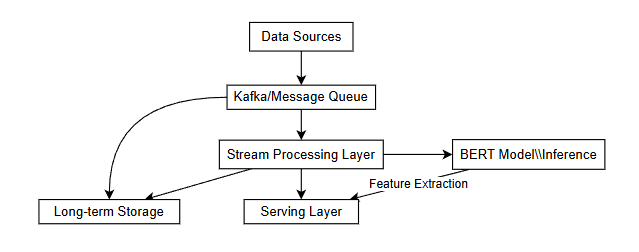
\includegraphics[width=1\textwidth]{Images/kappa_bert_architecture.png}
    \caption{Kiến trúc Kappa với BERT Model Integration}
    \label{fig:kappa_bert}
\end{figure}


\textbf{Các thành phần chính:}

\begin{enumerate}
    \item \textbf{Message Queue (Kafka)}: Nhận và lưu trữ tất cả dữ liệu đầu vào dưới dạng event log bất biến. Kafka đóng vai trò là single source of truth, cho phép replay dữ liệu khi cần thiết.
    
    \item \textbf{Stream Processing Layer}: Xử lý dữ liệu theo thời gian thực, thực hiện transformations, aggregations, và feature engineering cho BERT model.
    
    \item \textbf{ML Model Inference}: BERT model được deploy để thực hiện prediction trên streaming data.
    
    \item \textbf{Serving Layer}: Lưu trữ kết quả prediction và phục vụ các truy vấn từ applications.
    
    \item \textbf{Long-term Storage}: Lưu trữ dữ liệu lịch sử cho mục đích retraining model và analysis.
\end{enumerate}

\subsubsubsection{Apache Kafka làm backbone}

Apache Kafka là distributed streaming platform đóng vai trò trung tâm trong Kappa Architecture. Kafka được thiết kế như một commit log phân tán, nơi mọi message được lưu trữ theo thứ tự và có thể được đọc lại nhiều lần.

\textbf{Các khái niệm cốt lõi:}

\begin{itemize}
    \item \textbf{Topics}: Danh mục logic để phân loại messages. Ví dụ: traffic\_speed, traffic\_volume, traffic\_incidents.
    
    \item \textbf{Partitions}: Mỗi topic được chia thành nhiều partitions để tăng khả năng song song hóa và throughput.
    
    \item \textbf{Producers}: Các services ghi dữ liệu vào Kafka topics.
    
    \item \textbf{Consumers}: Các services đọc và xử lý dữ liệu từ topics.
    
    \item \textbf{Consumer Groups}: Nhóm consumers làm việc cùng nhau để xử lý song song dữ liệu từ một topic.
\end{itemize}

\textbf{Ưu điểm của Kafka trong hệ thống giao thông:}

\begin{itemize}
    \item \textbf{High Throughput}: Xử lý hàng triệu messages/giây từ các cảm biến giao thông
    \item \textbf{Durability}: Messages được replicate và persist, đảm bảo không mất dữ liệu
    \item \textbf{Scalability}: Dễ dàng scale horizontal bằng cách thêm brokers và partitions
    \item \textbf{Replay Capability}: Có thể đọc lại dữ liệu lịch sử để recompute hoặc fix bugs
    \item \textbf{Low Latency}: Độ trễ chỉ vài milliseconds, phù hợp cho real-time applications
\end{itemize}

\subsubsubsection{So sánh Kappa với Lambda Architecture}

\begin{table}[h]
\centering
\caption{So sánh Kappa và Lambda Architecture}
\begin{tabular}{|p{3.5cm}|p{5cm}|p{5cm}|}
\hline
\textbf{Tiêu chí} & \textbf{Lambda Architecture} & \textbf{Kappa Architecture} \\ \hline
Batch Layer & Có (MapReduce/Spark) & Không có \\ \hline
Speed Layer & Có (Stream Processing) & Stream processing duy nhất \\ \hline
Độ phức tạp & Cao (2 codebases riêng) & Thấp (1 codebase) \\ \hline
Độ trễ & Cao hơn do batch & Thấp, real-time \\ \hline
Consistency & Eventual consistency & Easier to maintain \\ \hline
Reprocessing & Cần chạy lại batch job & Replay từ Kafka \\ \hline
Maintenance & Khó (sync 2 systems) & Dễ hơn \\ \hline
Use case phù hợp & Cần cả batch và stream & Streaming-first applications \\ \hline
\end{tabular}
\label{tab:kappa_lambda}
\end{table}

\subsubsubsection{Ứng dụng Kappa trong hệ thống giao thông}

Trong bài toán phân tích giao thông, Kappa Architecture phù hợp vì:

\begin{enumerate}
    \item \textbf{Tính real-time}: Dữ liệu giao thông cần được xử lý ngay lập tức để cảnh báo kịp thời.
    
    \item \textbf{Data replay}: Khi cần retrain model hoặc fix bugs, có thể replay dữ liệu từ Kafka mà không cần maintain batch pipeline riêng.
    
    \item \textbf{Unified logic}: Cùng một đoạn code xử lý được sử dụng cho cả real-time và historical analysis.
    
    \item \textbf{Event-driven}: Giao thông là event-driven system (xe đi qua cảm biến, tắc nghẽn xảy ra, tai nạn), phù hợp với stream processing.
\end{enumerate}

\textbf{Pipeline xử lý trong hệ thống:}

\begin{enumerate}
    \item Cảm biến giao thông (camera, loop detectors, GPS) publish data vào Kafka topics
    \item Consumers đọc từ Kafka, thực hiện:
    \begin{itemize}
        \item Data cleaning và validation
        \item Feature extraction (tốc độ, volume, occupancy)
        \item Windowed aggregations (5-min, 15-min averages)
        \item Anomaly detection
        \item Correlation analysis
    \end{itemize}
    \item Kết quả được ghi vào:
    \begin{itemize}
        \item \textbf{Apache Parquet} (định dạng lưu trữ cột cho phân tích dữ liệu quy mô lớn)
    \end{itemize}
    \item ML models subscribe processed data để thực hiện predictions
    \item Results được publish lại vào Kafka để downstream services consume
\end{enumerate}
\subsubsection{TomTom Historical Traffic Stats API}

TomTom cung cấp dữ liệu giao thông lịch sử với độ bao phủ cao, bao gồm tốc độ trung bình, mức độ tắc nghẽn và chỉ số độ trễ theo từng đoạn đường. Dữ liệu được tổng hợp từ nhiều nguồn GPS và cập nhật theo khoảng thời gian từ 1--5 phút.

\paragraph{Ưu điểm}
\begin{itemize}
    \item Dữ liệu lịch sử dài hạn, hỗ trợ phân tích xu hướng theo giờ, ngày và tuần.
    \item Độ bao phủ rộng giúp bù đắp cho các khu vực thiếu cảm biến tại địa phương.
    \item Dễ dàng tích hợp vào các mô hình học chuỗi thời gian và mô hình mạng lưới.
\end{itemize}

\paragraph{Hạn chế}
\begin{itemize}
    \item Không phản ánh nguyên nhân của tắc nghẽn, chỉ mô tả hiện tượng.
    \item Chi phí sử dụng có thể cao nếu mở rộng cho toàn thành phố.
\end{itemize}

\paragraph{Vai trò trong đề tài}
Dữ liệu lịch sử từ TomTom giúp:
\begin{itemize}
    \item Huấn luyện mô hình dự báo giao thông.
    \item Phân tích lan truyền tắc nghẽn giữa các đoạn đường.
    \item Xây dựng dữ liệu đầu vào cho mô hình học sâu theo dạng đồ thị.
\end{itemize}

\subsubsection{Cơ sở dữ liệu và lưu trữ}

\subsubsubsection{Lưu trữ dữ liệu dạng cột với Apache Parquet}

Trong hệ thống phân tích giao thông đô thị, dữ liệu đầu vào có đặc trưng khối lượng lớn, cấu trúc rõ ràng và chủ yếu phục vụ cho các tác vụ phân tích, thống kê và huấn luyện mô hình học máy. Do đó, hệ thống lựa chọn \textbf{Apache Parquet} làm định dạng lưu trữ chính thay vì cơ sở dữ liệu giao dịch truyền thống.

Parquet là định dạng lưu trữ dạng cột (columnar storage), được thiết kế tối ưu cho các hệ thống phân tích dữ liệu lớn (Big Data Analytics) và các workload đọc nhiều, ghi ít.

\textbf{Các đặc điểm kỹ thuật chính của Parquet:}

\begin{itemize}
    \item \textbf{Columnar Storage}: Dữ liệu được lưu theo cột thay vì theo hàng, giúp giảm lượng dữ liệu cần đọc khi chỉ truy vấn một số thuộc tính cụ thể (ví dụ: tốc độ, lưu lượng, thời gian).
    
    \item \textbf{Efficient Compression}: Parquet hỗ trợ nhiều thuật toán nén (Snappy, ZSTD, GZIP), tận dụng tính đồng nhất của dữ liệu trong cùng một cột để đạt tỷ lệ nén cao, giảm đáng kể dung lượng lưu trữ.
    
    \item \textbf{Predicate Pushdown}: Cho phép loại bỏ sớm các block dữ liệu không thỏa điều kiện truy vấn, giúp tăng tốc độ xử lý.
    
    \item \textbf{Schema Evolution}: Hỗ trợ thay đổi schema theo thời gian (thêm/bớt cột) mà không làm hỏng dữ liệu cũ, phù hợp với dữ liệu giao thông có thể mở rộng thuộc tính.
    
    \item \textbf{Cross-platform Compatibility}: Tương thích tốt với các hệ sinh thái phân tích như Apache Spark, Pandas, DuckDB và các thư viện học máy.
\end{itemize}



\subsubsubsection{Ứng dụng Parquet trong hệ thống giao thông}

Trong hệ thống đề xuất, Parquet được sử dụng để lưu trữ các tập dữ liệu giao thông đã qua xử lý (processed data), bao gồm:

\begin{itemize}
    \item Thông tin các đoạn đường (road segments)
    \item Đặc trưng giao thông theo thời gian (speed, volume, congestion level)
    \item Dữ liệu đặc trưng đầu vào cho mô hình học máy
    \item Kết quả dự đoán và thống kê theo từng khung thời gian
\end{itemize}

Dữ liệu được tổ chức theo cấu trúc thư mục phân tầng dựa trên thời gian (theo ngày, giờ hoặc batch xử lý), giúp thuận tiện cho việc truy xuất, huấn luyện mô hình và phân tích hậu kỳ.
\subsubsection{API và Web Development Stack}

\subsubsubsection{FastAPI}

FastAPI là một web framework hiện đại dành cho Python, được thiết kế để xây dựng các dịch vụ API với hiệu năng cao, cú pháp rõ ràng và khả năng mở rộng tốt. Framework này đặc biệt phù hợp cho các hệ thống xử lý dữ liệu và mô hình học máy nhờ khả năng tích hợp chặt chẽ với hệ sinh thái Python.

\textbf{Các đặc điểm kỹ thuật chính của FastAPI:}

\begin{itemize}
    \item \textbf{High Performance}: FastAPI được xây dựng trên nền Starlette và Pydantic, cho hiệu năng xử lý cao, đáp ứng tốt các yêu cầu API có tần suất truy cập lớn.
    
    \item \textbf{Type-based Validation}: Sử dụng Python type hints để tự động kiểm tra, xác thực và chuyển đổi dữ liệu đầu vào, giúp giảm lỗi và tăng độ tin cậy của hệ thống.
    
    \item \textbf{Asynchronous Processing}: Hỗ trợ native \texttt{async/await}, cho phép xử lý đồng thời nhiều request, phù hợp với các pipeline phân tích dữ liệu và inference mô hình.
    
    \item \textbf{Automatic API Documentation}: Tự động sinh tài liệu OpenAPI (Swagger) và ReDoc, giúp việc kiểm thử và tích hợp API trở nên thuận tiện.
    
    \item \textbf{Modular Architecture}: Dễ dàng tổ chức code theo các module (router, service, schema), phù hợp cho các hệ thống nghiên cứu và phát triển mở rộng.
\end{itemize}

Trong hệ thống giao thông được đề xuất, FastAPI đóng vai trò là lớp trung gian cung cấp các API phục vụ:
\begin{itemize}
    \item Truy xuất dữ liệu giao thông đã được xử lý và lưu trữ dưới dạng Parquet
    \item Cung cấp đầu vào và đầu ra cho mô hình học máy
    \item Kết nối giữa pipeline xử lý dữ liệu và giao diện trực quan
\end{itemize}

\subsubsubsection{Streamlit}

Streamlit là framework Python nhẹ, được thiết kế để xây dựng nhanh các ứng dụng web phục vụ trực quan hóa dữ liệu và trình diễn kết quả phân tích mà không cần phát triển frontend phức tạp.

\textbf{Ưu điểm của Streamlit trong bối cảnh nghiên cứu và đồ án:}

\begin{itemize}
    \item \textbf{Rapid Prototyping}: Cho phép xây dựng giao diện trực quan chỉ với một lượng nhỏ mã Python, rút ngắn thời gian phát triển.
    
    \item \textbf{Tight Integration with Data Stack}: Tích hợp trực tiếp với Pandas, NumPy, PyArrow và các thư viện học máy, phù hợp cho việc hiển thị dữ liệu Parquet và kết quả mô hình.
    
    \item \textbf{Interactive Visualization}: Hỗ trợ tương tác người dùng theo thời gian thực (filter, slider, selection) cho các phân tích giao thông.
    
    \item \textbf{Lightweight Deployment}: Không yêu cầu quản lý state phức tạp hay frontend build system, phù hợp cho môi trường nghiên cứu và demo hệ thống.
\end{itemize}

Trong hệ thống này, Streamlit được sử dụng để:
\begin{itemize}
    \item Trực quan hóa dữ liệu giao thông theo không gian và thời gian
    \item Hiển thị kết quả dự đoán và phân tích của mô hình
    \item Phục vụ mục đích demo, đánh giá và trình bày hệ thống
\end{itemize}

Cách tiếp cận kết hợp FastAPI và Streamlit giúp tách biệt rõ ràng giữa lớp xử lý nghiệp vụ và lớp trình diễn, đảm bảo tính đơn giản, dễ bảo trì và phù hợp với mục tiêu nghiên cứu của đề tài.

\subsubsection{Containerization và Orchestration}

\subsubsubsection{Docker}

Docker là platform containerization cho phép đóng gói applications và dependencies thành containers độc lập, nhất quán trên mọi môi trường từ development đến production.

\textbf{Lợi ích của Docker:}

\begin{itemize}
    \item \textbf{Consistency}: "Works on my machine" problem được giải quyết
    \item \textbf{Isolation}: Mỗi service chạy trong môi trường riêng
    \item \textbf{Portability}: Deploy trên bất kỳ platform nào hỗ trợ Docker
    \item \textbf{Resource Efficiency}: Lightweight hơn VMs, chia sẻ kernel
    \item \textbf{Versioning}: Image versioning cho rollback dễ dàng
\end{itemize}

\textbf{Docker Compose} quản lý multi-container applications, định nghĩa toàn bộ stack (API, databases, cache, message queue) trong một file YAML, cho phép start/stop toàn bộ hệ thống với một command.

\subsubsubsection{Kubernetes}

Kubernetes (K8s) là container orchestration platform mã nguồn mở, tự động hóa việc deploy, scale, và manage containerized applications trong môi trường production.

\textbf{Khái niệm cốt lõi:}

\begin{itemize}
    \item \textbf{Pods}: Đơn vị nhỏ nhất, chứa một hoặc nhiều containers
    \item \textbf{ReplicaSets}: Đảm bảo số lượng pod replicas mong muốn
    \item \textbf{Deployments}: Quản lý rolling updates và rollbacks
    \item \textbf{Services}: Expose pods qua stable network endpoint
    \item \textbf{Ingress}: HTTP routing và load balancing
    \item \textbf{ConfigMaps và Secrets}: Quản lý configuration và sensitive data
    \item \textbf{Persistent Volumes}: Storage abstraction cho stateful apps
    \item \textbf{Namespaces}: Logical isolation giữa các môi trường
\end{itemize}

\textbf{Tính năng quan trọng cho production:}

\begin{enumerate}
    \item \textbf{Auto-scaling}: Horizontal Pod Autoscaler (HPA) tự động scale dựa trên CPU, memory, hoặc custom metrics
    
    \item \textbf{Self-healing}: Tự động restart failed containers, replace và reschedule pods khi nodes die
    
    \item \textbf{Service Discovery và Load Balancing}: Tự động distribute traffic đến healthy pods
    
    \item \textbf{Rolling Updates}: Zero-downtime deployments với progressive rollout
    
    \item \textbf{Resource Management}: CPU và memory requests/limits để optimize cluster utilization
\end{enumerate}

Với hệ thống giao thông cần high availability và khả năng scale dynamic theo traffic load, Kubernetes cung cấp infrastructure layer mạnh mẽ để đảm bảo reliability và performance.

\subsection{Tóm tắt stack công nghệ}

Bảng dưới đây tóm tắt các công nghệ chính được sử dụng trong đề tài:

\begin{table}[h]
\centering
\caption{Stack công nghệ hệ thống}
\begin{tabular}{|l|l|l|}
\hline
\textbf{Layer} & \textbf{Technology} & \textbf{Purpose} \\ \hline
Programming & Python 3.11+ & Main development language \\ \hline
ML Framework & PyTorch 2.0+ & Deep learning models \\ \hline
Graph Library & PyTorch Geometric & GNN implementation \\ \hline
Message Queue & Apache Kafka & Event streaming backbone \\ \hline
Stream Processing & Python + Kafka & Real-time data processing \\ \hline
Storage & Apache Parquet & Long-term historical data \\ \hline
% Cache & Redis & In-memory data store \\ \hline
Model Serving & FastAPI + PyTorch & Inference API \\ \hline
% Monitoring & Prometheus + Grafana & Metrics và visualization \\ \hline
\end{tabular}
\label{tab:tech_stack}
\end{table}

Kiến trúc này được thiết kế để:
\begin{itemize}
    \item Xử lý dữ liệu streaming real-time hiệu quả
    \item Scale horizontal khi traffic tăng
    \item Maintain low latency cho inference
    \item Support reprocessing và retraining
    \item Provide observability và monitoring đầy đủ
\end{itemize}


\newpage
\subsection{Kết chương}

Chương 2 đã trình bày một cách toàn diện nền tảng lý thuyết và công nghệ cần thiết để xây dựng hệ thống phân tích mối liên hệ giao thông đô thị. Những kiến thức này tạo thành bộ công cụ quan trọng phục vụ cho các chương tiếp theo của đồ án.

\textbf{Về mặt lý thuyết}, chúng ta đã nắm được:

\begin{itemize}
    \item Đặc điểm phức tạp của giao thông đô thị TP.HCM với cơ cấu phương tiện đặc thù, tỷ lệ xe máy chiếm ưu thế tuyệt đối (>90\%), và hiện tượng lan truyền tắc nghẽn theo mạng lưới đường. Việc hiểu rõ bản chất này giúp thiết kế mô hình phù hợp với đặc thù địa phương.

    \item Cơ sở toán học vững chắc về biểu diễn mạng giao thông dưới dạng đồ thị $\mathcal{G} = (\mathcal{V}, \mathcal{E}, \mathcal{A})$, các phép biến đổi trên cấu trúc đồ thị, và cách mô hình hóa tương quan không gian-thời gian.   

    \item Các kiến trúc Graph Neural Networks tiên tiến như GCN và GAT, cho phép học các mối quan hệ phức tạp giữa các nút giao thông mà không cần định nghĩa thủ công. Cơ chế message passing và attention mechanism là nền tảng để mô hình tự động phát hiện các mối tương quan ẩn.

    \item Các mô hình chuỗi thời gian từ RNN cơ bản đến LSTM và GRU, giúp nắm bắt phụ thuộc temporal với khả năng học long-term dependencies. Việc hiểu rõ ưu nhược điểm của từng loại giúp lựa chọn kiến trúc phù hợp cho bài toán dự báo đa bước (multi-step prediction).
\end{itemize}

\textbf{Về mặt công nghệ}, chương này đã xác định được bộ khung kỹ thuật (Technology Stack) hiện đại và mạnh mẽ để hiện thực hóa hệ thống:

\begin{itemize}
    \item \textbf{Hệ sinh thái Python \& PyTorch}: Cung cấp môi trường phát triển linh hoạt, đặc biệt là thư viện PyTorch Geometric chuyên dụng cho các mô hình GNN, giúp đơn giản hóa việc cài đặt các thuật toán phức tạp trên dữ liệu đồ thị.
    
    \item \textbf{Kiến trúc Kappa \& Apache Kafka}: Đảm bảo khả năng xử lý dữ liệu streaming thời gian thực với độ trễ thấp và độ tin cậy cao, phù hợp với đặc thù dữ liệu liên tục từ các cảm biến giao thông.
    
    \item \textbf{Lưu trữ dữ liệu không gian -- thời gian}: Hệ thống sử dụng định dạng Apache Parquet để lưu trữ dữ liệu giao thông có đặc trưng vừa mang thông tin không gian (tọa độ, đoạn đường), vừa mang tính chuỗi thời gian. Cách tiếp cận này cho phép tổ chức dữ liệu theo các phân vùng thời gian và thuộc tính không gian, đồng thời tối ưu hiệu năng cho các tác vụ phân tích, thống kê và huấn luyện mô hình học máy.
    
    \item \textbf{Hạ tầng triển khai}: Việc sử dụng Docker và Kubernetes đảm bảo hệ thống có khả năng mở rộng (scalability), dễ dàng triển khai và vận hành ổn định trong môi trường thực tế.
\end{itemize}

Sự kết hợp chặt chẽ giữa các nền tảng lý thuyết vững chắc và các công nghệ tiên tiến này là tiền đề quan trọng để bước sang Chương 3 -- nơi chúng ta sẽ khảo sát các công trình liên quan để định vị rõ hơn đóng góp của đề tài, và Chương 4 -- nơi mô hình hệ thống cụ thể sẽ được đề xuất.
\newpage
\section{Công trình liên quan}

Chương này trình bày tổng quan một cách có hệ thống về các nghiên cứu khoa học và hệ thống thực tế liên quan trực tiếp đến bài toán phân tích và dự báo giao thông đô thị. Nội dung được triển khai theo ba hướng chính: (1) tổng hợp các mô hình nghiên cứu từ truyền thống đến hiện đại; (2) phân tích các hệ thống lớn đang được vận hành trong thực tiễn; và (3) xác định các khoảng trống khoa học (gap) mà đề tài hướng đến giải quyết. Cách tiếp cận toàn diện này giúp đặt đề tài vào đúng bối cảnh phát triển của lĩnh vực, đồng thời làm rõ tính mới và đóng góp kỳ vọng của nghiên cứu.

\subsection{Các nghiên cứu liên quan}

\subsubsection{Mô hình hóa sự lan truyền và tắc nghẽn giao thông}

Các nghiên cứu nền tảng trong lĩnh vực giao thông trước thời kỳ học sâu chủ yếu dựa vào mô hình vật lý và thống kê nhằm mô tả bản chất lan truyền của dòng chảy giao thông. Những mô hình này giải thích cách tắc nghẽn hình thành, khuếch tán theo thời gian và ảnh hưởng lên các khu vực lân cận.

\subsubsubsection{Mô hình lan truyền sóng (Wave Propagation Models)}

Jiang và cộng sự nghiên cứu dữ liệu cảm biến tại Bắc Kinh và Thâm Quyến, qua đó xác định các \textit{jam centers}. Nhóm tác giả chỉ ra rằng tắc nghẽn lan truyền theo dạng sóng với vận tốc xấp xỉ $30 \pm 10$ km/h và cường độ suy giảm tuyến tính theo khoảng cách. Nghiên cứu cung cấp cơ sở thực nghiệm quan trọng giúp mô hình hóa tính chất không gian của tắc nghẽn.

\subsubsubsection{Mô hình lây lan (Contagion Process Models)}

Saberi và cộng sự tiếp cận theo hướng mô phỏng tắc nghẽn giao thông như một dạng bệnh dịch lây lan. Sử dụng mô hình SIR (Susceptible--Infected--Recovered), họ mô tả trạng thái ``nhiễm tắc nghẽn'' và ``hồi phục'' của các đoạn đường theo thời gian. Mô hình này hiệu quả ở cấp độ vĩ mô nhưng thiếu khả năng mô tả đặc trưng vi mô tại từng nút giao thông.

\subsubsubsection{Xác định nút thắt cổ chai (Bottleneck Detection)}

Li và cộng sự đề xuất phương pháp dựa trên lý thuyết đồ thị và chuỗi Markov nhằm xác định các nút thắt cổ chai dựa trên ``chi phí tắc nghẽn''. Chi phí này phản ánh không chỉ mức độ tắc tại một điểm mà còn khả năng lan truyền sang các đoạn khác. Đây là tư tưởng quan trọng được kế thừa trong đề tài khi đánh giá tác động liên vùng của các nút giao thông.

\subsubsection{Các mô hình Deep Learning với Ma trận kề tĩnh (Static Graph)}

Sự phát triển của Graph Convolutional Networks (GCN) mở ra phương pháp khai thác cấu trúc topo của mạng lưới giao thông để phục vụ dự báo.

\subsubsubsection{T-GCN}

Mô hình T-GCN kết hợp GCN và GRU để xử lý đồng thời thông tin không gian--thời gian. 

\begin{itemize}
    \item \textbf{Ưu điểm:} T-GCN vượt trội hơn các mô hình truyền thống như ARIMA hay SVR nhờ học trực tiếp đặc trưng topo của mạng lưới.
    \item \textbf{Hạn chế:} Ma trận kề $A$ được xây dựng tĩnh dựa trên khoảng cách hoặc kết nối vật lý, không phản ánh tính động của mối quan hệ giao thông theo thời gian.
\end{itemize}

\subsubsubsection{ST-GCN, DCRNN và các biến thể}

Các mô hình ST-GCN và DCRNN xử lý tốt hơn cơ chế khuếch tán, nhưng vẫn dựa trên đồ thị tĩnh đã được xác định trước. Điều này làm giảm hiệu quả trong bối cảnh giao thông phức tạp khi các mối quan hệ có thể thay đổi theo giờ cao điểm, sự cố, hoặc các yếu tố ngẫu nhiên khác.

\subsubsection{Các mô hình Deep Learning với Ma trận kề động (Dynamic Graph Learning)}

Nhằm khắc phục hạn chế của đồ thị tĩnh, các nghiên cứu gần đây tập trung vào xây dựng ma trận kề động, cập nhật theo từng thời điểm dựa trên dữ liệu thực nghiệm.

\subsubsubsection{DTC-STGCN}

Xu và cộng sự đề xuất mô hình DTC-STGCN, trong đó ma trận kề được tính toán động dựa trên tương quan giữa các nút qua từng thời điểm. Kết quả cho thấy độ chính xác dự báo tăng đáng kể nhờ mô hình hóa đúng bản chất thay đổi của mạng lưới giao thông.

\subsubsubsection{Attention và Graph Attention Networks (GAT)}

Cơ chế Attention giúp mô hình tự động học trọng số giữa các nút mà không cần ma trận kề định sẵn. Điều này đặc biệt phù hợp với bối cảnh TP.HCM, nơi tồn tại nhiều \textit{kết nối ngữ nghĩa} (semantic connections) không thể hiện bằng kết nối vật lý, ví dụ các nút giao thông xa nhau nhưng cùng nằm trên một luồng di chuyển chủ đạo.

\subsection{Các hệ thống và nền tảng thực tế}

\subsubsection{Google Maps và Waze}

Hai hệ thống này sử dụng dữ liệu khổng lồ từ cộng đồng, áp dụng các mô hình AI độ chính xác cao để dự báo thời gian thực. Tuy nhiên, chúng hoạt động như \textit{hộp đen}:
\begin{itemize}
    \item Không cung cấp khả năng phân tích nguyên nhân tắc nghẽn.
    \item Không hỗ trợ đánh giá mức độ lan truyền giữa các nút.
    \item Không phù hợp cho mục tiêu tối ưu hoá quản lý giao thông cấp thành phố.
\end{itemize}

\subsubsection{TomTom, Mapbox và các nền tảng bản đồ thương mại khác}

Bên cạnh Google Maps và Waze, còn có nhiều nền tảng bản đồ thương mại và dịch vụ dữ liệu giao thông chuyên sâu đóng vai trò quan trọng trong hệ sinh thái giao thông thông minh, tiêu biểu là TomTom, Mapbox, HERE, và INRIX. Các nền tảng này cung cấp tập hợp dịch vụ, API và dữ liệu có thể hỗ trợ cả ứng dụng điều hướng thương mại lẫn phân tích chuyên sâu cho nhà quản lý giao thông.

\paragraph{TomTom}
\begin{itemize}
    \item \textbf{Tính năng:} Cung cấp routing, traffic flow, traffic incidents, historical traffic, và map tiles. Hệ thống có dữ liệu thời gian thực và dữ liệu lịch sử được chuẩn hóa cho mục đích phân tích.
    \item \textbf{Nguồn dữ liệu:} Kết hợp dữ liệu cảm biến, probe data (điểm đo từ phương tiện), và hợp tác với nhà cung cấp địa phương.
    \item \textbf{Ưu điểm:} Chất lượng dữ liệu dành cho routing và dự báo thời gian đến (ETA) tốt; có các API chuyên nghiệp, SLA cho doanh nghiệp.
    \item \textbf{Hạn chế:} Dữ liệu thương mại (giấy phép) — chi phí có thể cao cho quy mô toàn thành phố; hạn chế về minh bạch (khó truy xuất nguồn gốc chi tiết từng điểm dữ liệu).
\end{itemize}

\paragraph{Mapbox}
\begin{itemize}
    \item \textbf{Tính năng:} Cung cấp công cụ hiển thị bản đồ (map rendering), vector tiles, routing, traffic overlays, và SDK cho frontend (web/mobile). Hỗ trợ tùy biến bản đồ cao, phù hợp cho dashboard và trực quan hoá.
    \item \textbf{Nguồn dữ liệu:} Kết hợp OpenStreetMap, dữ liệu đối tác, và các dịch vụ traffic provider để hiển thị trạng thái giao thông.
    \item \textbf{Ưu điểm:} Khả năng tuỳ biến giao diện bản đồ mạnh — phù hợp cho hệ thống giám sát và dashboard; dễ tích hợp với stack React/Deck.gl để hiển thị dữ liệu lớn.
    \item \textbf{Hạn chế:} Mapbox chủ yếu tập trung vào visualization và SDK — phần dữ liệu traffic chi tiết và phân tích nâng cao thường phụ thuộc vào nguồn bên thứ ba hoặc phải trả phí.
\end{itemize}

\paragraph{HERE Technologies}
\begin{itemize}
    \item \textbf{Tính năng:} Dịch vụ bản đồ, routing, traffic flow, incidents, map-matching, và rich telemetry. HERE có các API dành cho doanh nghiệp và hỗ trợ phân tích lịch sử/real-time.
    \item \textbf{Ưu điểm:} Strong enterprise features, hợp đồng dữ liệu cho thành phố, hỗ trợ map-matching chính xác — hữu ích khi kết hợp dữ liệu GPS/OBD.
    \item \textbf{Hạn chế:} Tương tự TomTom — chi phí và tính thương mại của dữ liệu cần cân nhắc.
\end{itemize}

\paragraph{INRIX}
\begin{itemize}
    \item \textbf{Tính năng:} Chuyên về dữ liệu lưu lượng và phân tích tắc nghẽn; cung cấp chỉ số congestion, travel time index, historical trend reports.
    \item \textbf{Ưu điểm:} Dữ liệu phân tích chuyên sâu, thuận lợi cho hoạch định chính sách và nghiên cứu dài hạn.
    \item \textbf{Hạn chế:} Chi phí bản quyền, không phải giải pháp “plug-and-play” cho các ứng dụng nhỏ.
\end{itemize}

\subsubsection*{So sánh ngắn gọn và vai trò trong hệ thống quản lý giao thông đô thị}

\begin{itemize}
    \item \textbf{Ứng dụng cho điều phối thành phố:} TomTom, HERE, và INRIX cung cấp dữ liệu và API đủ mạnh để phục vụ phân tích và báo cáo cấp thành phố (ví dụ: phân tích xu hướng, báo cáo tắc nghẽn theo chu kỳ). Tuy nhiên các dữ liệu này thường cần mua bản quyền và tích hợp bổ sung để phục vụ mục tiêu “giải thích lan truyền” (causal/spatio-temporal influence).
    \item \textbf{Ứng dụng cho trực quan hoá và giao diện:} Mapbox là lựa chọn thuận tiện để xây dựng dashboard tương tác và trực quan hoá dữ liệu thời gian thực (kết hợp với React, Deck.gl, hoặc Kepler.gl).
    \item \textbf{Tính mở và tích hợp với hệ thống nội bộ:} Nếu mục tiêu là nghiên cứu khoa học và mô hình hoá chi tiết (ví dụ: xây dựng ma trận kề động, chạy lại mô hình trên dữ liệu lịch sử), cần kết hợp dữ liệu thương mại này với nguồn nội địa (camera, loop detectors, GPS probe) và lưu trữ trong TimescaleDB/PostGIS. Dữ liệu thương mại nên được xem như \emph{một nguồn bổ trợ} chứ không thay thế hoàn toàn dữ liệu cảm biến tại chỗ.
    \item \textbf{Chi phí và pháp lý:} Các dịch vụ thương mại yêu cầu hợp đồng bản quyền và có thể giới hạn quyền sử dụng dữ liệu cho mục đích nghiên cứu/tái phân phối — yếu tố cần cân nhắc khi thiết kế kiến trúc dữ liệu mở cho thành phố.
\end{itemize}

\subsubsection{UTraffic}

UTraffic là nền tảng giám sát giao thông thời gian thực thông qua camera và cảm biến. Hệ thống đang thực hiện tốt chức năng giám sát, nhưng vẫn còn khoảng trống lớn trong:
\begin{itemize}
    \item phân tích sâu (deep analysis),
    \item dự báo thời gian dài,
    \item và mô hình hóa lan truyền tắc nghẽn.
\end{itemize}

\subsection{Khoảng trống nghiên cứu (Gap Analysis)}

Dựa trên tổng quan các công trình và hệ thống thực tế, có thể xác định ba khoảng trống chính:

\begin{enumerate}
    \item \textbf{Hạn chế của ma trận kề tĩnh:} Các mô hình hiện tại như T-GCN vẫn sử dụng đồ thị tĩnh, không phản ánh đúng mối quan hệ động giữa các nút giao thông trong các đô thị phức tạp như TP.HCM.
    
    \item \textbf{Thiếu nghiên cứu cho giao thông hỗn hợp:} Phần lớn công trình quốc tế nghiên cứu trên dữ liệu ô tô hoặc taxi, vốn có luồng di chuyển tổ chức. TP.HCM lại có đặc thù xe máy chiếm đa số, tạo ra tính hỗn loạn (chaotic) cao.
    
    \item \textbf{Nhu cầu chuyển từ dự báo sang giải thích:} Các mô hình hiện tại chủ yếu báo trước tắc nghẽn, nhưng chưa giải thích được cơ chế lan truyền và mức độ ảnh hưởng giữa các nút -- điều cần thiết cho hoạch định chiến lược.
\end{enumerate}

\subsection*{Tóm tắt}

Chương này đã phân tích toàn diện các công trình nghiên cứu và hệ thống thực tế trong lĩnh vực giao thông. Những khoảng trống được xác định là cơ sở quan trọng để đề tài lựa chọn hướng tiếp cận: \textbf{cải tiến T-GCN bằng cơ chế học ma trận kề động (Dynamic Graph Learning)}, từ đó nâng cao khả năng dự báo và phân tích lan truyền tắc nghẽn trên dữ liệu giao thông thực tế tại TP.HCM.


\newpage
\section{Phương pháp giải quyết}

Chương này trình bày chi tiết phương pháp luận và các bước thực hiện để giải quyết bài toán phân tích mối liên hệ giao thông giữa các nút quan trọng tại TP.HCM. Phương pháp được thiết kế dựa trên nền tảng lý thuyết đã trình bày ở Chương 2 và các khoảng trống nghiên cứu được xác định ở Chương 3, đồng thời tận dụng dữ liệu lịch sử từ TomTom Historical Traffic Stats API.

\subsection{Tổng quan phương pháp tiếp cận}

\subsubsection{Định hướng giải pháp}

Để giải quyết bài toán phân tích mối liên hệ và lan truyền tắc nghẽn giữa các nút giao thông, đề tài đề xuất một pipeline xử lý toàn diện kết hợp nhiều kỹ thuật từ Big Data, Deep Learning, và phân tích thống kê. Giải pháp tập trung vào ba mục tiêu chính:

\begin{enumerate}
    \item \textbf{Phát hiện tương quan không gian-thời gian}: Xác định các cặp nút giao thông có mức độ ảnh hưởng lẫn nhau cao, định lượng độ mạnh của mối tương quan và xác định độ trễ lan truyền.
    
    \item \textbf{Xác định quan hệ nhân quả}: Phân biệt mối tương quan đơn thuần và quan hệ nhân-quả thực sự, xác định nút nào là nguyên nhân gây ra tắc nghẽn lan truyền.
    
    \item \textbf{Dự báo lan truyền tắc nghẽn}: Xây dựng mô hình có khả năng dự báo khi một nút giao thông bị tắc nghẽn sẽ lan truyền đến các nút nào và trong bao lâu.
\end{enumerate}

\subsubsection{Kiến trúc tổng thể}

Hệ thống được thiết kế theo kiến trúc phân tầng, mỗi tầng đảm nhiệm một nhóm chức năng cụ thể:

\begin{figure}[h]
\centering
\begin{tikzpicture}[node distance=1.5cm, scale=0.9, transform shape]
% Data Layer
\node[draw, rectangle, minimum width=10cm, minimum height=1.2cm, fill=blue!10] (data) {
    \textbf{Data Layer}: TomTom API, Data Collection, Storage
};

% Processing Layer
\node[draw, rectangle, minimum width=10cm, minimum height=1.2cm, fill=green!10, below of=data, yshift=-0.5cm] (processing) {
    \textbf{Processing Layer}: Data Cleaning, Feature Engineering, Aggregation
};

% Analysis Layer
\node[draw, rectangle, minimum width=10cm, minimum height=1.2cm, fill=orange!10, below of=processing, yshift=-0.5cm] (analysis) {
    \textbf{Analysis Layer}: Correlation Analysis, Causality Testing
};

% Model Layer
\node[draw, rectangle, minimum width=10cm, minimum height=1.2cm, fill=red!10, below of=analysis, yshift=-0.5cm] (model) {
    \textbf{Model Layer}: Dynamic GCN, Temporal Modeling, Prediction
};

% Application Layer
\node[draw, rectangle, minimum width=10cm, minimum height=1.2cm, fill=purple!10, below of=model, yshift=-0.5cm] (app) {
    \textbf{Application Layer}: Visualization, Alerting, Reporting
};

% Arrows
\draw[->, thick] (data) -- (processing);
\draw[->, thick] (processing) -- (analysis);
\draw[->, thick] (analysis) -- (model);
\draw[->, thick] (model) -- (app);

% Feedback loop
\draw[->, thick, dashed] (model.east) -- ++(1.5,0) |- (processing.east);
\node[right, text width=2cm] at (11.5, -3) {\small Model Feedback};

\end{tikzpicture}
\caption{Kiến trúc tổng thể hệ thống}
\label{fig:overall_architecture}
\end{figure}

\subsubsection{Quy trình xử lý chính}

Pipeline xử lý dữ liệu và phân tích được thực hiện theo trình tự sau:

\begin{enumerate}
    \item \textbf{Thu thập dữ liệu}: Lấy dữ liệu lịch sử từ TomTom API cho các nút giao thông được chọn
    \item \textbf{Tiền xử lý}: Làm sạch, chuẩn hóa, và xử lý missing values
    \item \textbf{Trích xuất đặc trưng}: Tính toán các đặc trưng giao thông và thời gian
    \item \textbf{Phân tích tương quan}: Xác định mối tương quan không gian-thời gian
    \item \textbf{Kiểm định nhân quả}: Áp dụng Granger Causality Test
    \item \textbf{Xây dựng đồ thị động}: Tạo ma trận kề thay đổi theo thời gian
    \item \textbf{Huấn luyện mô hình}: Phát triển mô hình dự báo dựa trên GNN
    \item \textbf{Đánh giá và triển khai}: Kiểm thử và tích hợp vào hệ thống
\end{enumerate}

\newpage
\subsection{Thu thập và chuẩn bị dữ liệu}

\subsubsection{Nguồn dữ liệu: TomTom Historical Traffic Stats}

\subsubsubsection{Lý do lựa chọn TomTom API}

Dữ liệu giao thông lịch sử từ TomTom được lựa chọn làm nguồn dữ liệu chính cho đề tài vì các lý do sau:

\begin{itemize}
    \item \textbf{Độ phủ toàn diện}: TomTom cung cấp dữ liệu cho hầu hết các tuyến đường chính tại TP.HCM, bao gồm cả các khu vực trung tâm và vùng ven.
    
    \item \textbf{Chất lượng dữ liệu}: Dữ liệu được tổng hợp từ nhiều nguồn (GPS probe data, cảm biến, crowdsourcing) và đã qua xử lý, lọc nhiễu bởi TomTom.
    
    \item \textbf{Dữ liệu lịch sử dài hạn}: API cung cấp dữ liệu lịch sử từ nhiều tháng đến nhiều năm, đủ để huấn luyện mô hình học sâu.
    
    \item \textbf{Độ phân giải thời gian phù hợp}: Dữ liệu có độ phân giải 5 phút, cân bằng giữa chi tiết và khả năng xử lý.
    
    \item \textbf{Các chỉ số phong phú}: Bao gồm tốc độ thực tế, tốc độ tự do, thời gian di chuyển, độ tin cậy, giúp phân tích đa chiều.
\end{itemize}

\subsubsubsection{Cấu trúc dữ liệu TomTom}

TomTom Historical Traffic Stats API cung cấp dữ liệu theo cấu trúc sau:

\begin{itemize}
    \item \textbf{Road Segments}: Mỗi đoạn đường được định danh bởi segment ID duy nhất
    \item \textbf{Temporal Resolution}: Dữ liệu theo khung thời gian 5 phút
    \item \textbf{Speed Metrics}:
    \begin{itemize}
        \item \texttt{currentSpeed}: Tốc độ trung bình thực tế (km/h)
        \item \texttt{freeFlowSpeed}: Tốc độ tự do khi không có tắc nghẽn (km/h)
        \item \texttt{confidence}: Độ tin cậy của số liệu (0-1)
    \end{itemize}
    \item \textbf{Congestion Indicators}:
    \begin{itemize}
        \item \texttt{travelTime}: Thời gian di chuyển thực tế (giây)
        \item \texttt{freeFlowTravelTime}: Thời gian di chuyển lý tưởng (giây)
    \end{itemize}
    \item \textbf{Metadata}: Thông tin đoạn đường (tên đường, tọa độ, chiều dài)
\end{itemize}

\subsubsection{Lựa chọn nút giao thông nghiên cứu}

\subsubsubsection{Tiêu chí lựa chọn}

Việc lựa chọn các nút giao thông để nghiên cứu dựa trên các tiêu chí sau:

\begin{enumerate}
    \item \textbf{Tầm quan trọng chiến lược}:
    \begin{itemize}
        \item Nút nằm trên các tuyến huyết mạch nối các quận trung tâm
        \item Cổng vào/ra khu vực trung tâm TP.HCM
        \item Giao lộ có lưu lượng cao và thường xuyên ùn tắc
    \end{itemize}
    
    \item \textbf{Độ phủ dữ liệu}:
    \begin{itemize}
        \item Đảm bảo có dữ liệu TomTom liên tục cho đoạn đường
        \item Tỷ lệ missing data dưới 10\%
        \item Độ tin cậy trung bình (confidence) trên 0.7
    \end{itemize}
    
    \item \textbf{Tính đại diện}:
    \begin{itemize}
        \item Phân bố đều trong khu vực nghiên cứu
        \item Bao gồm nhiều loại đường: đại lộ, đường chính, đường nhánh
        \item Đa dạng về mật độ giao thông và đặc điểm vận hành
    \end{itemize}
    
    \item \textbf{Khả năng kết nối}:
    \begin{itemize}
        \item Có mối liên hệ trực tiếp hoặc gián tiếp với các nút khác
        \item Nằm trong cùng một mạng lưới liên thông
    \end{itemize}
\end{enumerate}

\subsubsubsection{Danh sách nút giao thông được chọn}

Dựa trên các tiêu chí trên, đề tài lựa chọn 20 nút giao thông trọng điểm tại TP.HCM, bao gồm:

\begin{table}[h]
\centering
\caption{Các nút giao thông được lựa chọn}
\begin{tabular}{|l|l|l|}
\hline
\textbf{STT} & \textbf{Tên nút/đường} & \textbf{Khu vực} \\ \hline
1 & Ngã ba Cách Mạng Tháng 8 - Điện Biên Phủ & Quận 3 \\ \hline
2 & Ngã tư Hàng Xanh & Quận Bình Thạnh \\ \hline
3 & Cầu Sài Gòn & Quận 1 - Quận 4 \\ \hline
4 & Đường Võ Văn Kiệt (đoạn Q1) & Quận 1 \\ \hline
5 & Ngã tư Bảy Hiền & Quận Tân Bình \\ \hline
6 & Xa lộ Hà Nội (đoạn Q9) & Quận 9 \\ \hline
7 & Đại lộ Võ Văn Kiệt (đoạn Q5) & Quận 5 \\ \hline
8 & Nguyễn Thị Minh Khai & Quận 1, Quận 3 \\ \hline
9 & Cầu Kênh Tẻ & Quận 1 - Quận 7 \\ \hline
10 & Đường 3 Tháng 2 & Quận 10, Quận 11 \\ \hline
... & ... & ... \\ \hline
\end{tabular}
\label{tab:selected_nodes}
\end{table}

\subsubsection{Quy trình thu thập dữ liệu}

\subsubsubsection{Thiết kế data pipeline}

Pipeline thu thập dữ liệu được thiết kế để đảm bảo tính ổn định, hiệu quả và khả năng mở rộng:

\begin{figure}[h]
\centering
\begin{tikzpicture}[node distance=2.5cm, scale=0.85, transform shape]

% Nodes
\node[draw, rectangle, rounded corners, minimum width=3cm] (api) {TomTom API};
\node[draw, rectangle, rounded corners, minimum width=3cm, below of=api] (collector) {Data Collector};
\node[draw, rectangle, rounded corners, minimum width=3cm, below of=collector] (validator) {Validator};
\node[draw, rectangle, rounded corners, minimum width=3cm, below of=validator] (storage) {PostgreSQL};

% Parallel processes
\node[draw, rectangle, rounded corners, minimum width=2.5cm, right of=collector, xshift=3cm] (retry) {Retry Logic};
\node[draw, rectangle, rounded corners, minimum width=2.5cm, right of=validator, xshift=3cm] (logger) {Error Logger};

% Arrows
\draw[->, thick] (api) -- (collector) node[midway, right] {JSON Response};
\draw[->, thick] (collector) -- (validator) node[midway, right] {Raw Data};
\draw[->, thick] (validator) -- (storage) node[midway, right] {Clean Data};

\draw[->, dashed] (collector) -- (retry);
\draw[->, dashed] (retry) |- (api);
\draw[->, dashed] (validator) -- (logger);

% Labels
\node[right of=api, xshift=2cm, text width=2.5cm, align=left] {\small Rate Limit: 100 req/hour};
\node[right of=storage, xshift=2cm, text width=2.5cm, align=left] {\small TimescaleDB for time-series};

\end{tikzpicture}
\caption{Pipeline thu thập dữ liệu từ TomTom API}
\label{fig:data_collection_pipeline}
\end{figure}

\subsubsubsection{Các bước thu thập}

\begin{enumerate}
    \item \textbf{Xác định time range}:
    \begin{itemize}
        \item Thu thập dữ liệu từ 01-8-2024 đến 31-8-2024
        \item Độ phân giải: 5 phút/lần đo
        \item Tập trung vào giờ cao điểm: 6h-9h, 17h-20h
    \end{itemize}
    
    \item \textbf{API Request Strategy}:
    \begin{itemize}
        \item Batch requests để tối ưu số lần gọi API
        \item Implement exponential backoff khi gặp rate limit
        \item Cache responses để tránh duplicate requests
    \end{itemize}
    
    \item \textbf{Data Validation}:
    \begin{itemize}
        \item Kiểm tra completeness: đảm bảo đủ các trường bắt buộc
        \item Kiểm tra consistency: tốc độ không âm, trong giới hạn hợp lý
        \item Kiểm tra temporal continuity: không có gaps lớn giữa các measurements
    \end{itemize}
    
    \item \textbf{Error Handling}:
    \begin{itemize}
        \item Log tất cả errors để phân tích sau
        \item Retry failed requests với backoff strategy
        \item Alert khi error rate vượt threshold
    \end{itemize}
\end{enumerate}

\subsubsection{Tiền xử lý dữ liệu}

\subsubsubsection{Xử lý missing values}

Dữ liệu giao thông thực tế thường có missing values do nhiều nguyên nhân: lỗi cảm biến, mất kết nối, hoặc không đủ probe data. Chiến lược xử lý:

\begin{enumerate}
    \item \textbf{Phân loại missing patterns}:
    \begin{itemize}
        \item \textit{MCAR (Missing Completely At Random)}: Xảy ra ngẫu nhiên
        \item \textit{MAR (Missing At Random)}: Phụ thuộc vào biến quan sát được
        \item \textit{MNAR (Missing Not At Random)}: Phụ thuộc vào giá trị bị missing
    \end{itemize}
    
    \item \textbf{Phương pháp imputation}:
    \begin{itemize}
        \item \textbf{Linear Interpolation}: Cho gaps nhỏ (< 3 time steps)
        \[
        v_t = v_{t-1} + \frac{v_{t+k} - v_{t-1}}{k+1}
        \]
        
        \item \textbf{Seasonal Decomposition}: Cho gaps trung bình
        \[
        v_t = \text{trend}_t + \text{seasonal}_t + \text{residual}_t
        \]
        
        \item \textbf{KNN Imputation}: Dựa vào các nút láng giềng tương tự
        \[
        v_t^i = \frac{1}{k}\sum_{j \in \text{KNN}(i)} v_t^j \cdot w_{ij}
        \]
        
        \item \textbf{Deep Learning Imputation}: Sử dụng LSTM autoencoder cho gaps lớn
    \end{itemize}
    
    \item \textbf{Quality threshold}:
    \begin{itemize}
        \item Loại bỏ nút có > 20\% missing data
        \item Đánh dấu imputed values để đánh giá độ tin cậy
    \end{itemize}
\end{enumerate}

\subsubsubsection{Outlier detection và xử lý}

Outliers trong dữ liệu giao thông có thể do tai nạn, sự kiện đặc biệt, hoặc lỗi đo:

\begin{enumerate}
    \item \textbf{Statistical Methods}:
    \begin{itemize}
        \item \textbf{Z-score}: Phát hiện điểm bất thường dựa trên độ lệch chuẩn
        \[
        z_i = \frac{x_i - \mu}{\sigma}, \quad |z_i| > 3 \Rightarrow \text{outlier}
        \]
        
        \item \textbf{IQR (Interquartile Range)}:
        \[
        \text{outlier if } x < Q_1 - 1.5 \cdot \text{IQR} \text{ or } x > Q_3 + 1.5 \cdot \text{IQR}
        \]
    \end{itemize}
    
    \item \textbf{Temporal Context}:
    \begin{itemize}
        \item So sánh với cùng thời điểm các ngày trước
        \item Xem xét xu hướng và mùa vụ
        \item Kiểm tra consistency với nút láng giềng
    \end{itemize}
    
    \item \textbf{Handling Strategy}:
    \begin{itemize}
        \item \textbf{Keep}: Nếu có bằng chứng là sự kiện thực (tai nạn, sự kiện)
        \item \textbf{Cap}: Giới hạn trong khoảng hợp lý
        \item \textbf{Remove}: Nếu xác định là lỗi đo
        \item \textbf{Flag}: Đánh dấu để phân tích riêng
    \end{itemize}
\end{enumerate}

\subsubsubsection{Normalization và scaling}

Chuẩn hóa dữ liệu là bước quan trọng để mô hình học hiệu quả:

\begin{enumerate}
    \item \textbf{Min-Max Scaling}:
    \[
    x_{\text{norm}} = \frac{x - x_{\min}}{x_{\max} - x_{\min}}
    \]
    Sử dụng cho features có phân phối đồng đều, giữ nguyên shape.
    
    \item \textbf{Z-score Standardization}:
    \[
    x_{\text{std}} = \frac{x - \mu}{\sigma}
    \]
    Phù hợp khi features có phân phối gần Gaussian.
    
    \item \textbf{Robust Scaling}:
    \[
    x_{\text{robust}} = \frac{x - \text{median}}{\text{IQR}}
    \]
    Ít bị ảnh hưởng bởi outliers.
\end{enumerate}

Lựa chọn phương pháp dựa trên:
\begin{itemize}
    \item Phân phối của từng feature
    \item Yêu cầu của model (GNN, LSTM thường cần standardization)
    \item Presence of outliers
\end{itemize}

\newpage
\subsection{Trích xuất và phân tích đặc trưng}

\subsubsection{Đặc trưng giao thông cơ bản}

\subsubsubsection{Speed-based features}

Từ dữ liệu TomTom, trích xuất các đặc trưng liên quan đến tốc độ:

\begin{enumerate}
    \item \textbf{Relative Speed}:
    \[
    v_{\text{rel}}(t) = \frac{v_{\text{current}}(t)}{v_{\text{freeflow}}}
    \]
    Chỉ số này phản ánh mức độ tắc nghẽn, với giá trị gần 1 nghĩa là lưu thông tốt.
    
    \item \textbf{Speed Reduction Ratio}:
    \[
    r_{\text{reduction}}(t) = 1 - v_{\text{rel}}(t) = \frac{v_{\text{freeflow}} - v_{\text{current}}(t)}{v_{\text{freeflow}}}
    \]
    Tỷ lệ giảm tốc độ so với lý tưởng.
    
    \item \textbf{Congestion Index}:
    \[
    CI(t) = \frac{t_{\text{travel}}(t)}{t_{\text{freeflow}}} - 1
    \]
    Chỉ số tắc nghẽn dựa trên tỷ lệ thời gian di chuyển tăng thêm.
    
    \item \textbf{Speed Variance}:
    \[
    \sigma_v^2 = \frac{1}{n}\sum_{i=1}^n (v_i - \bar{v})^2
    \]
    Độ biến động tốc độ phản ánh tính không ổn định của giao thông.
\end{enumerate}

\subsubsubsection{Temporal features}

Các đặc trưng theo thời gian giúp mô hình nhận biết patterns chu kỳ:

\begin{enumerate}
    \item \textbf{Time of Day Features}:
    \begin{itemize}
        \item Hour of day: $h \in [0, 23]$
        \item Minute of hour: $m \in [0, 59]$
        \item Cyclic encoding để giữ tính liên tục:
        \[
        h_{\sin} = \sin\left(\frac{2\pi h}{24}\right), \quad h_{\cos} = \cos\left(\frac{2\pi h}{24}\right)
        \]
    \end{itemize}
    
    \item \textbf{Day of Week Features}:
    \begin{itemize}
        \item Weekday vs Weekend (binary)
        \item Day of week: $d \in [0, 6]$
        \item Cyclic encoding tương tự
    \end{itemize}
    
    \item \textbf{Peak/Off-peak Indicator}:
    \[
    \text{isPeak}(t) = 
    \begin{cases}
        1, & \text{if } t \in [6, 9] \cup [16, 19] \\
        0, & \text{otherwise}
    \end{cases}
    \]
\end{enumerate}

\subsubsection{Đặc trưng không gian}

\subsubsubsection{Spatial proximity features}

Tính toán các đặc trưng về mối quan hệ không gian giữa các nút:

\begin{enumerate}
    \item \textbf{Euclidean Distance}:
    \[
    d_{\text{euclid}}(i, j) = \sqrt{(x_i - x_j)^2 + (y_i - y_j)^2}
    \]
    
    \item \textbf{Road Network Distance}:
    \[
    d_{\text{network}}(i, j) = \text{shortest\_path\_length}(i, j)
    \]
    Khoảng cách thực tế theo mạng đường, tính bằng thuật toán Dijkstra.
    
    \item \textbf{Travel Time Distance}:
    \[
    d_{\text{time}}(i, j) = \mathbb{E}[t_{\text{travel}}(i \to j)]
    \]
    Khoảng cách dựa trên thời gian di chuyển trung bình.
    
    \item \textbf{Connectivity Features}:
    \begin{itemize}
        \item Direct connection: Binary indicator
        \item Number of intermediate nodes
        \item Betweenness centrality: Đo lường tầm quan trọng của nút trong mạng
    \end{itemize}
\end{enumerate}

\subsubsubsection{Neighborhood aggregation}

Tổng hợp thông tin từ các nút láng giềng:

\begin{enumerate}
    \item \textbf{Spatial Average}:
    \[
    \bar{v}_i^{\text{spatial}}(t) = \frac{1}{|\mathcal{N}_i|}\sum_{j \in \mathcal{N}_i} v_j(t)
    \]
    
    \item \textbf{Weighted Spatial Average}:
    \[
    \bar{v}_i^{\text{weighted}}(t) = \frac{\sum_{j \in \mathcal{N}_i} w_{ij} \cdot v_j(t)}{\sum_{j \in \mathcal{N}_i} w_{ij}}
    \]
    với trọng số $w_{ij} = \exp(-d_{ij}/\sigma)$ dựa trên khoảng cách.
    
    \item \textbf{Spatial Variance}:
    \[
    \sigma_i^{\text{spatial}}(t) = \sqrt{\frac{1}{|\mathcal{N}_i|}\sum_{j \in \mathcal{N}_i} (v_j(t) - \bar{v}_i^{\text{spatial}}(t))^2}
    \]
\end{enumerate}

\subsubsection{Đặc trưng động học (Dynamic Features)}

\subsubsubsection{Temporal derivatives}

Các đạo hàm theo thời gian phản ánh xu hướng thay đổi của giao thông:

\begin{enumerate}
    \item \textbf{First-order Derivative (Velocity)}:
    \[
    \frac{dv}{dt} \approx \frac{v(t) - v(t-1)}{\Delta t}
    \]
    Tốc độ thay đổi của traffic speed, cho biết giao thông đang cải thiện hay xấu đi.
    
    \item \textbf{Second-order Derivative (Acceleration)}:
    \[
    \frac{d^2v}{dt^2} \approx \frac{v(t) - 2v(t-1) + v(t-2)}{\Delta t^2}
    \]
    Gia tốc thay đổi, hữu ích để phát hiện điểm chuyển pha (từ thông sang tắc).
    
    \item \textbf{Rate of Change}:
    \[
    r_{\text{change}}(t) = \frac{v(t) - v(t-k)}{v(t-k)} \times 100\%
    \]
    Phần trăm thay đổi so với $k$ bước thời gian trước.
\end{enumerate}

\subsubsubsection{Trend and momentum features}

\begin{enumerate}
    \item \textbf{Moving Average}:
    \[
    \text{MA}_k(t) = \frac{1}{k}\sum_{i=0}^{k-1} v(t-i)
    \]
    Làm mượt nhiễu và phát hiện xu hướng.
    
    \item \textbf{Exponential Moving Average}:
    \[
    \text{EMA}_{\alpha}(t) = \alpha \cdot v(t) + (1-\alpha) \cdot \text{EMA}_{\alpha}(t-1)
    \]
    Cho trọng số cao hơn cho dữ liệu gần đây.
    
    \item \textbf{Momentum}:
    \[
    M(t) = v(t) - v(t-k)
    \]
    Đo lường sức mạnh của xu hướng.
    
    \item \textbf{Volatility}:
    \[
    \text{Vol}(t) = \sqrt{\frac{1}{k}\sum_{i=0}^{k-1}(v(t-i) - \text{MA}_k(t))^2}
    \]
    Độ dao động trong window thời gian.
\end{enumerate}

\subsubsection{Đặc trưng tương quan sơ bộ}

Trước khi áp dụng các phương pháp phức tạp, tính toán tương quan ban đầu:

\begin{enumerate}
    \item \textbf{Pearson Correlation}:
    \[
    \rho_{ij} = \frac{\text{Cov}(X_i, X_j)}{\sigma_{X_i}\sigma_{X_j}}
    \]
    Đo lường tương quan tuyến tính giữa hai nút.
    
    \item \textbf{Time-lagged Correlation}:
    \[
    \rho_{ij}(\tau) = \text{Corr}(X_i(t), X_j(t+\tau))
    \]
    Tương quan với độ trễ $\tau$, giúp xác định delay trong lan truyền.
    
    \item \textbf{Cross-correlation Function}:
    \[
    \text{CCF}_{ij}(\tau) = \frac{\mathbb{E}[(X_i(t) - \mu_i)(X_j(t+\tau) - \mu_j)]}{\sigma_i \sigma_j}
    \]
\end{enumerate}

\newpage
\subsection{Phân tích tương quan không gian-thời gian}

\subsubsection{Phương pháp phân tích tương quan}

\subsubsubsection{Dynamic Time Warping (DTW)}

DTW đo lường độ tương đồng giữa hai chuỗi thời gian có thể bị lệch về thời gian:

\begin{enumerate}
    \item \textbf{Định nghĩa DTW Distance}:
    
    Cho hai chuỗi $X = (x_1, x_2, \ldots, x_n)$ và $Y = (y_1, y_2, \ldots, y_m)$, DTW tìm alignment path tối ưu:
    \[
    \text{DTW}(X, Y) = \min_{\pi} \sqrt{\sum_{(i,j) \in \pi} d(x_i, y_j)^2}
    \]
    
    \item \textbf{Thuật toán quy hoạch động}:
    \[
    D(i, j) = d(x_i, y_j) + \min\{D(i-1, j), D(i, j-1), D(i-1, j-1)\}
    \]
    
    \item \textbf{Ứng dụng trong giao thông}:
    \begin{itemize}
        \item Phát hiện patterns tương tự giữa các nút mặc dù có time shift
        \item Xác định propagation delay giữa các nút
        \item Clustering các nút có behavior tương đồng
    \end{itemize}
\end{enumerate}

\subsubsubsection{Wavelet Coherence Analysis}

Wavelet coherence phân tích tương quan trong cả miền thời gian và tần số:

\begin{enumerate}
    \item \textbf{Continuous Wavelet Transform}:
    \[
    W_x(a, b) = \frac{1}{\sqrt{|a|}}\int_{-\infty}^{\infty} x(t)\psi^*\left(\frac{t-b}{a}\right)dt
    \]
    với $a$ là scale parameter, $b$ là translation parameter.
    
    \item \textbf{Wavelet Coherence}:
    \[
    R^2(a, b) = \frac{|S(W_{xy}(a,b))|^2}{S(|W_x(a,b)|^2) \cdot S(|W_y(a,b)|^2)}
    \]
    với $S$ là smoothing operator.
    
    \item \textbf{Phase Difference}:
    \[
    \phi_{xy}(a, b) = \arctan\left(\frac{\Im\{W_{xy}(a,b)\}}{\Re\{W_{xy}(a,b)\}}\right)
    \]
    Cho biết nút nào dẫn trước (leading) và nút nào theo sau (lagging).
\end{enumerate}

\subsubsection{Xây dựng ma trận tương quan}

\subsubsubsection{Static correlation matrix}

Ma trận tương quan tĩnh được tính trên toàn bộ dữ liệu:

\begin{enumerate}
    \item \textbf{Pearson Correlation Matrix}:
    \[
    C_{ij} = \frac{\sum_{t=1}^T (x_i(t) - \bar{x}_i)(x_j(t) - \bar{x}_j)}{\sqrt{\sum_{t=1}^T(x_i(t) - \bar{x}_i)^2}\sqrt{\sum_{t=1}^T(x_j(t) - \bar{x}_j)^2}}
    \]
    
    \item \textbf{Distance Correlation}:
    \[
    \text{dCor}(X, Y) = \frac{\text{dCov}(X, Y)}{\sqrt{\text{dCov}(X, X) \cdot \text{dCov}(Y, Y)}}
    \]
    Distance correlation có thể phát hiện cả quan hệ phi tuyến.
    
    \item \textbf{Mutual Information}:
    \[
    I(X; Y) = \sum_{x \in X}\sum_{y \in Y} p(x, y)\log\frac{p(x, y)}{p(x)p(y)}
    \]
    Đo lường mức độ phụ thuộc tổng quát, không giới hạn tuyến tính.
\end{enumerate}

\subsubsubsection{Time-varying correlation matrix}

Ma trận tương quan động thay đổi theo thời gian:

\begin{enumerate}
    \item \textbf{Rolling Window Correlation}:
    \[
    C_{ij}(t) = \text{Corr}(X_i[t-w:t], X_j[t-w:t])
    \]
    với $w$ là window size.
    
    \item \textbf{Exponentially Weighted Correlation}:
    \[
    C_{ij}(t) = \frac{\sum_{k=0}^{t} \lambda^k (x_i(t-k) - \bar{x}_i)(x_j(t-k) - \bar{x}_j)}{\sqrt{\sum_{k=0}^{t}\lambda^k(x_i(t-k) - \bar{x}_i)^2}\sqrt{\sum_{k=0}^{t}\lambda^k(x_j(t-k) - \bar{x}_j)^2}}
    \]
    
    \item \textbf{State-dependent Correlation}:
    \[
    C_{ij}^{(s)} = \text{Corr}(X_i | S=s, X_j | S=s)
    \]
    Tương quan phụ thuộc vào trạng thái giao thông (normal, congested, incident).
\end{enumerate}

\subsubsection{Xác định độ trễ lan truyền}

\subsubsubsection{Cross-correlation analysis}

\begin{enumerate}
    \item \textbf{Tính CCF cho nhiều lags}:
    \[
    \text{CCF}_{ij}(\tau) = \text{Corr}(X_i(t), X_j(t + \tau)), \quad \tau \in [-\tau_{\max}, \tau_{\max}]
    \]
    
    \item \textbf{Xác định optimal lag}:
    \[
    \tau^*_{ij} = \operatorname*{arg\,max}_{\tau} |\text{CCF}_{ij}(\tau)|
    \]
    
    \item \textbf{Interpretation}:
    \begin{itemize}
        \item Nếu $\tau^*_{ij} > 0$: nút $i$ dẫn trước nút $j$ (influence direction $i \to j$)
        \item Nếu $\tau^*_{ij} < 0$: nút $j$ dẫn trước nút $i$ (influence direction $j \to i$)
        \item $|\tau^*_{ij}|$ là độ trễ lan truyền (propagation delay)
    \end{itemize}
\end{enumerate}

\subsubsubsection{Transfer Entropy}

Transfer Entropy đo lường lượng thông tin truyền từ nút này sang nút khác:

\begin{equation}
TE_{i \to j} = \sum p(x_j^{t+1}, x_j^{(k)}, x_i^{(l)}) \log \frac{p(x_j^{t+1}|x_j^{(k)}, x_i^{(l)})}{p(x_j^{t+1}|x_j^{(k)})}
\end{equation}

với:
\begin{itemize}
    \item $x_j^{(k)} = (x_j^t, x_j^{t-1}, \ldots, x_j^{t-k+1})$: lịch sử của nút $j$
    \item $x_i^{(l)} = (x_i^t, x_i^{t-1}, \ldots, x_i^{t-l+1})$: lịch sử của nút $i$
\end{itemize}

Transfer Entropy cao nghĩa là nút $i$ mang thông tin dự báo hữu ích cho nút $j$.

\newpage
\subsection{Kiểm định quan hệ nhân quả}

\subsubsection{Granger Causality Test}

\subsubsubsection{Cơ sở lý thuyết}

Granger Causality dựa trên ý tưởng: nếu $X$ gây ra $Y$, thì giá trị quá khứ của $X$ sẽ giúp dự báo tốt hơn giá trị tương lai của $Y$, so với chỉ dùng giá trị quá khứ của $Y$.

\begin{enumerate}
    \item \textbf{Unrestricted Model}:
    \[
    Y_t = \alpha_0 + \sum_{i=1}^p \alpha_i Y_{t-i} + \sum_{j=1}^q \beta_j X_{t-j} + \epsilon_t
    \]
    
    \item \textbf{Restricted Model}:
    \[
    Y_t = \alpha_0 + \sum_{i=1}^p \alpha_i Y_{t-i} + \eta_t
    \]
    
    \item \textbf{Test Statistic}:
    \[
    F = \frac{(\text{RSS}_R - \text{RSS}_U)/q}{\text{RSS}_U/(T - p - q - 1)}
    \]
    với RSS là residual sum of squares.
    
    \item \textbf{Null Hypothesis}: $H_0: \beta_1 = \beta_2 = \cdots = \beta_q = 0$ (X không Granger-cause Y)
    
    \item \textbf{Decision}: Nếu $p\text{-value} < \alpha$ (thường 0.05), reject $H_0$, kết luận X Granger-causes Y.
\end{enumerate}

\subsubsubsection{Pairwise Granger Causality}

Thực hiện kiểm định cho tất cả các cặp nút:

\begin{enumerate}
    \item \textbf{Test $i \to j$}: Kiểm tra liệu nút $i$ có Granger-cause nút $j$ không
    \item \textbf{Test $j \to i$}: Kiểm tra chiều ngược lại
    \item \textbf{Kết quả có thể}:
    \begin{itemize}
        \item Unidirectional: $i \to j$ hoặc $j \to i$
        \item Bidirectional: $i \leftrightarrow j$ (ảnh hưởng lẫn nhau)
        \item No causality: không có quan hệ nhân quả
    \end{itemize}
\end{enumerate}

\subsubsubsection{Lag selection}

Việc chọn số lag $p$ và $q$ quan trọng cho độ chính xác:

\begin{enumerate}
    \item \textbf{Akaike Information Criterion (AIC)}:
    \[
    \text{AIC}(p) = 2k - 2\ln(\hat{L})
    \]
    với $k$ là số tham số, $\hat{L}$ là likelihood.
    
    \item \textbf{Bayesian Information Criterion (BIC)}:
    \[
    \text{BIC}(p) = k\ln(n) - 2\ln(\hat{L})
    \]
    
    \item \textbf{Strategy}:
    \begin{itemize}
        \item Test với nhiều giá trị lag khác nhau
        \item Chọn lag có AIC hoặc BIC nhỏ nhất
        \item Xem xét domain knowledge (propagation thường trong 15-30 phút)
    \end{itemize}
\end{enumerate}

\subsubsection{Conditional Granger Causality}

Trong mạng lưới phức tạp, cần kiểm soát ảnh hưởng của các nút khác:

\begin{enumerate}
    \item \textbf{Model với conditioning}:
    \[
    Y_t = \alpha_0 + \sum_{i=1}^p \alpha_i Y_{t-i} + \sum_{j=1}^q \beta_j X_{t-j} + \sum_{k=1}^r \gamma_k Z_{t-k} + \epsilon_t
    \]
    với $Z$ là các nút điều kiện.
    
    \item \textbf{Ứng dụng}:
    \begin{itemize}
        \item Phát hiện spurious causality do confounding variables
        \item Xác định direct vs indirect influence
        \item Tìm mediating nodes trong propagation path
    \end{itemize}
\end{enumerate}

\subsubsection{Xây dựng Causal Graph}

\subsubsubsection{Từ kết quả kiểm định đến đồ thị}

\begin{enumerate}
    \item \textbf{Adjacency Matrix Construction}:
    \[
    A^{\text{causal}}_{ij} = 
    \begin{cases}
        1, & \text{if } i \text{ Granger-causes } j \text{ (significant)} \\
        0, & \text{otherwise}
    \end{cases}
    \]
    
    \item \textbf{Weighted Causal Graph}:
    \[
    W^{\text{causal}}_{ij} = F\text{-statistic}_{i \to j} \text{ or } 1 - p\text{-value}_{i \to j}
    \]
    
    \item \textbf{Thresholding}:
    \begin{itemize}
        \item Giữ chỉ các edges có $p\text{-value} < 0.05$
        \item Hoặc giữ top-k strongest causal links
        \item Hoặc dùng FDR (False Discovery Rate) correction cho multiple testing
    \end{itemize}
\end{enumerate}

\subsubsubsection{Graph properties analysis}

Phân tích các tính chất của causal graph:

\begin{enumerate}
    \item \textbf{In-degree và Out-degree}:
    \[
    d^{\text{in}}_j = \sum_{i=1}^N A^{\text{causal}}_{ij}, \quad d^{\text{out}}_i = \sum_{j=1}^N A^{\text{causal}}_{ij}
    \]
    \begin{itemize}
        \item High out-degree: nút là "source" của tắc nghẽn (influential node)
        \item High in-degree: nút dễ bị ảnh hưởng (vulnerable node)
    \end{itemize}
    
    \item \textbf{Betweenness Centrality}:
    \[
    BC(v) = \sum_{s \neq v \neq t} \frac{\sigma_{st}(v)}{\sigma_{st}}
    \]
    với $\sigma_{st}$ là số shortest paths từ $s$ đến $t$, $\sigma_{st}(v)$ là số paths đi qua $v$.
    
    Nút có BC cao là "bottleneck" trong propagation network.
    
    \item \textbf{PageRank}:
    \[
    PR(i) = \frac{1-d}{N} + d\sum_{j \in \text{In}(i)} \frac{PR(j)}{d^{\text{out}}_j}
    \]
    Đánh giá tầm quan trọng của nút trong mạng causal.
\end{enumerate}

\newpage
\subsection{Xây dựng mô hình dự báo}

\subsubsection{Kiến trúc Dynamic Graph Convolutional Network}

\subsubsubsection{Motivation}

Các mô hình T-GCN truyền thống sử dụng ma trận kề tĩnh $A$, không phản ánh:
\begin{itemize}
    \item Sự thay đổi của mối quan hệ theo thời gian
    \item Ảnh hưởng của trạng thái giao thông hiện tại lên cấu trúc mạng
    \item Các mối liên hệ tiềm ẩn không thể hiện qua kết nối vật lý
\end{itemize}

Do đó, đề tài đề xuất Dynamic GCN với ma trận kề được học và cập nhật theo thời gian.

\subsubsubsection{Dynamic Adjacency Matrix Learning}

\textbf{Adaptive Graph Learning:}

\begin{enumerate}
    \item \textbf{Node Embedding}:
    
    Mỗi nút $i$ được biểu diễn bởi một embedding vector học được:
    \[
    \mathbf{e}_i \in \mathbb{R}^d
    \]
    
    \item \textbf{Similarity-based Adjacency}:
    \[
    A_{ij}^{(t)} = \frac{\exp(\text{sim}(\mathbf{h}_i^{(t)}, \mathbf{h}_j^{(t)}))}{\sum_{k=1}^N \exp(\text{sim}(\mathbf{h}_i^{(t)}, \mathbf{h}_k^{(t)}))}
    \]
    
    với $\text{sim}(\cdot, \cdot)$ có thể là:
    \begin{itemize}
        \item Cosine similarity: $\text{sim}(\mathbf{u}, \mathbf{v}) = \frac{\mathbf{u}^T\mathbf{v}}{\|\mathbf{u}\|\|\mathbf{v}\|}$
        \item Scaled dot-product: $\text{sim}(\mathbf{u}, \mathbf{v}) = \frac{\mathbf{u}^T\mathbf{v}}{\sqrt{d}}$
        \item Bilinear: $\text{sim}(\mathbf{u}, \mathbf{v}) = \mathbf{u}^T\mathbf{W}\mathbf{v}$
    \end{itemize}
    
    \item \textbf{Hybrid Adjacency Matrix}:
    
    Kết hợp cả thông tin cấu trúc và dữ liệu:
    \[
    A^{(t)} = \alpha A^{\text{static}} + (1-\alpha)A^{\text{dynamic}}(t)
    \]
    
    với:
    \begin{itemize}
        \item $A^{\text{static}}$: ma trận kề dựa trên cấu trúc đường (prior knowledge)
        \item $A^{\text{dynamic}}(t)$: ma trận học được từ dữ liệu tại thời điểm $t$
        \item $\alpha \in [0,1]$: hyperparameter cân bằng
    \end{itemize}
\end{enumerate}

\textbf{Attention-based Graph Construction:}

Sử dụng cơ chế attention để học trọng số động:

\begin{equation}
\alpha_{ij}^{(t)} = \frac{\exp(\text{LeakyReLU}(\mathbf{a}^T[\mathbf{W}\mathbf{h}_i^{(t)} \| \mathbf{W}\mathbf{h}_j^{(t)}]))}{\sum_{k \in \mathcal{N}_i} \exp(\text{LeakyReLU}(\mathbf{a}^T[\mathbf{W}\mathbf{h}_i^{(t)} \| \mathbf{W}\mathbf{h}_k^{(t)}]))}
\end{equation}

với $\|$ là concatenation operation.

\subsubsubsection{Temporal Modeling Component}

\textbf{GRU Cell với Dynamic Graph:}

Tại mỗi time step $t$:

\begin{align}
\mathbf{X}_t' &= \text{GraphConv}(A^{(t)}, \mathbf{X}_t) \\
\mathbf{r}_t &= \sigma(\mathbf{W}_r[\mathbf{X}_t', \mathbf{h}_{t-1}] + \mathbf{b}_r) \\
\mathbf{u}_t &= \sigma(\mathbf{W}_u[\mathbf{X}_t', \mathbf{h}_{t-1}] + \mathbf{b}_u) \\
\tilde{\mathbf{h}}_t &= \tanh(\mathbf{W}_h[\mathbf{X}_t', \mathbf{r}_t \odot \mathbf{h}_{t-1}] + \mathbf{b}_h) \\
\mathbf{h}_t &= \mathbf{u}_t \odot \mathbf{h}_{t-1} + (1 - \mathbf{u}_t) \odot \tilde{\mathbf{h}}_t
\end{align}

\textbf{Multi-scale Temporal Attention:}

Để nắm bắt dependencies ở nhiều time scales:

\begin{equation}
\mathbf{h}_t^{\text{multi}} = \text{Concat}[\mathbf{h}_t^{\text{short}}, \mathbf{h}_t^{\text{medium}}, \mathbf{h}_t^{\text{long}}]
\end{equation}

với:
\begin{itemize}
    \item $\mathbf{h}_t^{\text{short}}$: GRU trên window 12 steps (1 giờ)
    \item $\mathbf{h}_t^{\text{medium}}$: GRU trên window 36 steps (3 giờ)
    \item $\mathbf{h}_t^{\text{long}}$: GRU trên window 144 steps (12 giờ)
\end{itemize}

\subsubsubsection{Kiến trúc tổng thể}

\begin{figure}[h]
\centering
\begin{tikzpicture}[
    node distance=1.6cm,
    every node/.style={draw, rectangle, minimum width=2.6cm, align=center},
    >=Stealth
]

% Input
\node (input) {Input $\mathbf{X}_{t-T:t}$};

% Dynamic Graph Learning
\node[below=of input, fill=yellow!20] (graph)
{Dynamic Graph\\Learning};

% Spatial Component
\node[below=of graph, fill=blue!20] (spatial)
{Graph Convolution\\Layers};

% Temporal Component
\node[below=of spatial, fill=green!20] (temporal)
{GRU\\Layers};

% Multi-scale Attention
\node[right=of temporal, xshift=1.8cm, fill=orange!20] (multiscale)
{Multi-scale\\Attention};

% Output
\node[below=of temporal, yshift=-0.4cm] (output)
{Output $\hat{\mathbf{Y}}_{t+1:t+H}$};

% Arrows
\draw[->, thick] (input) -- (graph);
\draw[->, thick] (graph) -- node[right] {$A^{(t)}$} (spatial);
\draw[->, thick] (spatial) -- (temporal);
\draw[->, thick] (temporal) -- (output);

\draw[->, dashed] (temporal) -- (multiscale);
\draw[->, dashed] (multiscale) |- (output);

% Side annotations
\node[right=of graph, xshift=2.2cm, text width=3.2cm, draw=none]
{\small Learn time-varying\\adjacency matrix};

\node[right=of spatial, xshift=2.2cm, text width=3.2cm, draw=none]
{\small Capture spatial\\dependencies};

\node[right=of output, xshift=2.2cm, text width=3.2cm, draw=none]
{\small Multi-step\\forecasting};

\end{tikzpicture}
\caption{Kiến trúc mô hình Dynamic GCN với học đồ thị động và mô hình hóa thời gian đa tầng}
\label{fig:dynamic_gcn_architecture}
\end{figure}

\subsubsection{Training Strategy}

\subsubsubsection{Loss Function}

Hàm mất mát kết hợp nhiều objectives:

\begin{equation}
\mathcal{L}_{\text{total}} = \mathcal{L}_{\text{pred}} + \lambda_1\mathcal{L}_{\text{graph}} + \lambda_2\mathcal{L}_{\text{reg}}
\end{equation}

\textbf{1. Prediction Loss:}

\[
\mathcal{L}_{\text{pred}} = \frac{1}{NH}\sum_{i=1}^N\sum_{h=1}^H \|\mathbf{y}_i^{(t+h)} - \hat{\mathbf{y}}_i^{(t+h)}\|_2^2
\]

Hoặc sử dụng Huber loss để robust hơn với outliers:

\[
\mathcal{L}_{\text{Huber}}(\delta) = 
\begin{cases}
\frac{1}{2}(y - \hat{y})^2, & |y - \hat{y}| \leq \delta \\
\delta|y - \hat{y}| - \frac{1}{2}\delta^2, & |y - \hat{y}| > \delta
\end{cases}
\]

\textbf{2. Graph Regularization Loss:}

Để đảm bảo ma trận kề học được có tính chất tốt:

\[
\mathcal{L}_{\text{graph}} = \|A^{(t)} - A^{(t-1)}\|_F^2 + \lambda_{\text{sparse}}\|A^{(t)}\|_1
\]

\begin{itemize}
    \item Term 1: Temporal smoothness - ma trận kề không thay đổi quá đột ngột
    \item Term 2: Sparsity - khuyến khích mạng thưa, chỉ giữ connections quan trọng
\end{itemize}

\textbf{3. Regularization Loss:}

\[
\mathcal{L}_{\text{reg}} = \|\boldsymbol{\theta}\|_2^2
\]

L2 regularization cho tất cả parameters để tránh overfitting.

\subsubsubsection{Optimization Algorithm}

\textbf{Adam Optimizer với Learning Rate Scheduling:}

\begin{enumerate}
    \item \textbf{Base optimizer}: Adam với parameters:
    \begin{itemize}
        \item Initial learning rate: $\eta_0 = 0.001$
        \item $\beta_1 = 0.9$, $\beta_2 = 0.999$
        \item $\epsilon = 10^{-8}$
    \end{itemize}
    
    \item \textbf{Learning rate schedule}:
    \[
    \eta_t = \eta_0 \cdot \min\left(1, \frac{\text{warmup\_steps}}{t}\right) \cdot 0.5^{\lfloor t/\text{decay\_steps}\rfloor}
    \]
    
    \begin{itemize}
        \item Warmup period: 1000 steps để ổn định training
        \item Decay: giảm 50% mỗi 5000 steps
    \end{itemize}
    
    \item \textbf{Gradient clipping}:
    \[
    \mathbf{g} \leftarrow \min\left(1, \frac{\text{max\_norm}}{\|\mathbf{g}\|}\right) \mathbf{g}
    \]
    với $\text{max\_norm} = 5.0$ để tránh exploding gradients.
\end{enumerate}

\subsubsubsection{Training Procedure}

\begin{enumerate}
    \item \textbf{Data Splitting}:
    \begin{itemize}
        \item Training set: 70\% (dữ liệu cũ nhất)
        \item Validation set: 15\% (dữ liệu giữa)
        \item Test set: 15\% (dữ liệu mới nhất)
        \item Temporal split - không shuffle để giữ tính thời gian
    \end{itemize}
    
    \item \textbf{Training Loop}:
    \begin{itemize}
        \item Batch size: 32 sequences
        \item Input window: 12 time steps (1 giờ)
        \item Prediction horizon: 12 time steps (1 giờ)
        \item Early stopping: patience = 20 epochs
        \item Model checkpoint: lưu best model theo validation loss
    \end{itemize}
    
    \item \textbf{Data Augmentation}:
    \begin{itemize}
        \item Add Gaussian noise: $\mathbf{X}' = \mathbf{X} + \mathcal{N}(0, 0.01)$
        \item Time masking: randomly mask một số time steps
        \item Node masking: randomly mask features của một số nodes
    \end{itemize}
\end{enumerate}

\subsubsection{Model Ensemble}

Để tăng độ robust, sử dụng ensemble của nhiều models:

\begin{enumerate}
    \item \textbf{Multiple Seeds}: Train 5 models với random seeds khác nhau
    
    \item \textbf{Ensemble Prediction}:
    \[
    \hat{\mathbf{y}}_{\text{ensemble}} = \frac{1}{K}\sum_{k=1}^K w_k \hat{\mathbf{y}}_k
    \]
    
    với weights $w_k$ có thể là:
    \begin{itemize}
        \item Uniform: $w_k = 1/K$
        \item Performance-based: $w_k \propto 1/\text{MAE}_k^{\text{val}}$
    \end{itemize}
    
    \item \textbf{Uncertainty Quantification}:
    \[
    \sigma^2_{\text{ensemble}} = \frac{1}{K}\sum_{k=1}^K (\hat{\mathbf{y}}_k - \hat{\mathbf{y}}_{\text{ensemble}})^2
    \]
    
    Variance của predictions cho biết độ tin cậy của dự báo.
\end{enumerate}

\newpage
\subsection{Hệ thống cảnh báo và phát hiện lan truyền}

\subsubsection{Thuật toán phát hiện bất thường}

\subsubsubsection{Threshold-based Detection}

\textbf{Định nghĩa trạng thái tắc nghẽn:}

\[
\text{Congestion Level} = 
\begin{cases}
\text{Free Flow}, & \text{if } CI(t) < 0.2 \\
\text{Moderate}, & \text{if } 0.2 \leq CI(t) < 0.5 \\
\text{Heavy}, & \text{if } 0.5 \leq CI(t) < 0.8 \\
\text{Severe}, & \text{if } CI(t) \geq 0.8
\end{cases}
\]

với $CI(t) = \frac{t_{\text{travel}}(t)}{t_{\text{freeflow}}} - 1$ là Congestion Index.

\textbf{Multi-level Thresholds:}

\begin{itemize}
    \item \textbf{Speed-based}: 
    \[
    v_{\text{rel}}(t) < \tau_v \Rightarrow \text{Congested}
    \]
    với $\tau_v = 0.6$ (tốc độ dưới 60\% tốc độ tự do)
    
    \item \textbf{Trend-based}:
    \[
    \frac{dv}{dt} < -\tau_{\Delta v} \Rightarrow \text{Deteriorating}
    \]
    Phát hiện xu hướng giảm tốc độ nhanh
\end{itemize}

\subsubsubsection{Statistical Anomaly Detection}

\textbf{Z-score Method:}

\[
z_i(t) = \frac{v_i(t) - \mu_i}{\sigma_i}
\]

\[
\text{Anomaly if } |z_i(t)| > \theta_z
\]

với $\theta_z = 3$ (3-sigma rule).

\textbf{Isolation Forest:}

Sử dụng ensemble of random trees để phát hiện điểm bất thường:
\begin{itemize}
    \item Anomalies có average path length ngắn hơn
    \item Anomaly score:
    \[
    s(x, n) = 2^{-\frac{E(h(x))}{c(n)}}
    \]
    với $h(x)$ là path length, $c(n)$ là normalization factor
\end{itemize}

\subsubsection{Mô hình lan truyền}

\subsubsubsection{Cascade Prediction Model}

Khi phát hiện tắc nghẽn tại nút $i$ ở thời điểm $t_0$, dự đoán xác suất lan truyền:

\begin{equation}
P(j \text{ congested at } t | i \text{ congested at } t_0) = f(A_{ij}, \tau_{ij}, \mathbf{h}_j(t))
\end{equation}

với:
\begin{itemize}
    \item $A_{ij}$: causal influence strength từ $i$ đến $j$
    \item $\tau_{ij}$: propagation delay
    \item $\mathbf{h}_j(t)$: current state của nút $j$
\end{itemize}

\textbf{Logistic Regression Model:}

\[
P(y_j = 1 | \mathbf{x}) = \frac{1}{1 + \exp(-(\beta_0 + \beta_1 A_{ij} + \beta_2 v_j + \beta_3 d_{ij}))}
\]

\textbf{Neural Network Classifier:}

Input features:
\begin{itemize}
    \item Causal influence $A_{ij}$
    \item Current speed $v_j(t)$
    \item Distance $d_{ij}$
    \item Time of day
    \item Historical congestion patterns
\end{itemize}

Output: Probability of congestion at different time horizons ($t+15$min, $t+30$min, $t+60$min).

\subsubsubsection{Graph-based Propagation Simulation}

Sử dụng causal graph để mô phỏng lan truyền:

\begin{algorithm}[h]
\caption{Congestion Propagation Simulation}
\label{alg:congestion_propagation}
\begin{algorithmic}[1]

\Require Causal graph $G$, initial congested node $i_0$, time horizon $T$
\Ensure Set of affected nodes at each time step

\State $\text{Congested}[0] \gets \{i_0\}$

\For{$t = 1$ to $T$}
    \State $\text{Congested}[t] \gets \text{Congested}[t-1]$
    \ForAll{$i \in \text{Congested}[t-1]$}
        \ForAll{$j$ such that $A_{ij} > 0$}
            \If{$t - t_0 \ge \tau_{ij}$ \textbf{and} $P_{\text{spread}}(i \rightarrow j) > \theta$}
                \State $\text{Congested}[t] \gets \text{Congested}[t] \cup \{j\}$
            \EndIf
        \EndFor
    \EndFor
\EndFor

\State \Return $\text{Congested}[1:T]$

\end{algorithmic}
\end{algorithm}

\subsubsection{Hệ thống cảnh báo đa cấp}

\subsubsubsection{Alert Severity Levels}

\begin{table}[h]
\centering
\caption{Mức độ cảnh báo}
\begin{tabular}{|l|l|l|}
\hline
\textbf{Level} & \textbf{Condition} & \textbf{Action} \\ \hline
\textcolor{green}{Info} & Moderate congestion, localized & Log and monitor \\ \hline
\textcolor{orange}{Warning} & Heavy congestion, risk of spreading & Alert operators \\ \hline
\textcolor{red}{Critical} & Severe congestion, cascading & Immediate intervention \\ \hline
\textcolor{purple}{Emergency} & Multiple critical nodes, network failure & Emergency protocol \\ \hline
\end{tabular}
\label{tab:alert_levels}
\end{table}

\subsubsubsection{Alert Content}

Mỗi alert bao gồm:

\begin{itemize}
    \item \textbf{Source Node}: Nút gốc bị tắc nghẽn
    \item \textbf{Affected Nodes}: Danh sách nút có nguy cơ bị ảnh hưởng
    \item \textbf{Estimated Impact Time}: Thời điểm dự kiến tắc nghẽn lan đến từng nút
    \item \textbf{Severity Score}: Mức độ nghiêm trọng tổng hợp
    \item \textbf{Recommended Actions}: Các biện pháp đề xuất
    \item \textbf{Confidence Level}: Độ tin cậy của dự báo
\end{itemize}

\subsubsubsection{Alert Routing}

\begin{itemize}
    \item \textbf{Dashboard}: Real-time visualization cho control center
    \item \textbf{Mobile App}: Push notifications cho traffic officers
    \item \textbf{API}: Integration với các hệ thống khác (VMS, traffic lights)
    \item \textbf{Email/SMS}: Notifications cho stakeholders
\end{itemize}

\newpage
\subsection{Đánh giá và metrics}

\subsubsection{Metrics cho dự báo}

\subsubsubsection{Point Prediction Metrics}

\textbf{1. Mean Absolute Error (MAE):}

\[
\text{MAE} = \frac{1}{N \cdot H}\sum_{i=1}^N\sum_{h=1}^H |y_i^{(t+h)} - \hat{y}_i^{(t+h)}|
\]

Đo lường sai số trung bình, ít bị ảnh hưởng bởi outliers.

\textbf{2. Root Mean Squared Error (RMSE):}

\[
\text{RMSE} = \sqrt{\frac{1}{N \cdot H}\sum_{i=1}^N\sum_{h=1}^H (y_i^{(t+h)} - \hat{y}_i^{(t+h)})^2}
\]

Penalize lỗi lớn mạnh hơn MAE.

\textbf{3. Mean Absolute Percentage Error (MAPE):}

\[
\text{MAPE} = \frac{100\%}{N \cdot H}\sum_{i=1}^N\sum_{h=1}^H \left|\frac{y_i^{(t+h)} - \hat{y}_i^{(t+h)}}{y_i^{(t+h)}}\right|
\]

Đo lường sai số tương đối, dễ interpret.

\textbf{4. $R^2$ Score:}

\[
R^2 = 1 - \frac{\sum_i (y_i - \hat{y}_i)^2}{\sum_i (y_i - \bar{y})^2}
\]

Tỷ lệ variance được giải thích bởi mô hình.

\subsubsubsection{Distribution Prediction Metrics}

Cho probabilistic predictions:

\textbf{1. Continuous Ranked Probability Score (CRPS):}

\[
\text{CRPS}(F, y) = \int_{-\infty}^{\infty}(F(x) - \mathbb{1}\{x \geq y\})^2 dx
\]

với $F$ là cumulative distribution function của prediction.

\textbf{2. Prediction Interval Coverage Probability (PICP):}

\[
\text{PICP} = \frac{1}{N}\sum_{i=1}^N \mathbb{1}\{y_i \in [L_i, U_i]\}
\]

Tỷ lệ true values nằm trong prediction interval $[L_i, U_i]$.

\subsubsection{Metrics cho phát hiện tương quan}

\subsubsubsection{Correlation Detection Accuracy}

So sánh với ground truth (nếu có) hoặc expert knowledge:

\textbf{1. Precision và Recall:}

\[
\text{Precision} = \frac{TP}{TP + FP}, \quad \text{Recall} = \frac{TP}{TP + FN}
\]

\[
F_1 = 2 \cdot \frac{\text{Precision} \cdot \text{Recall}}{\text{Precision} + \text{Recall}}
\]

với:
\begin{itemize}
    \item TP: Correctly identified correlations
    \item FP: Falsely identified correlations
    \item FN: Missed correlations
\end{itemize}

\textbf{2. Area Under ROC Curve (AUC-ROC):}

Đánh giá khả năng phân biệt giữa correlated và uncorrelated pairs.

\subsubsubsection{Causal Discovery Accuracy}

\textbf{1. Structural Hamming Distance (SHD):}

\[
\text{SHD}(G_{\text{true}}, G_{\text{pred}}) = |E_{\text{true}} \triangle E_{\text{pred}}| + |E_{\text{reversed}}|
\]

Đếm số edges sai khác (missing, extra, reversed).

\textbf{2. F1 Score for Causal Edges:}

Tính precision, recall trên directed edges.

\subsubsection{Metrics cho cảnh báo}

\subsubsubsection{Alert Quality Metrics}

\textbf{1. True Positive Rate (Detection Rate):}

\[
\text{TPR} = \frac{\text{\# correct alerts}}{\text{\# actual events}}
\]

\textbf{2. False Positive Rate:}

\[
\text{FPR} = \frac{\text{\# false alerts}}{\text{\# non-events}}
\]

\textbf{3. Lead Time:}

\[
\text{Lead Time} = t_{\text{alert}} - t_{\text{event}}
\]

Thời gian cảnh báo trước khi sự kiện xảy ra (càng lớn càng tốt, nhưng không quá lớn để tránh false alarms).

\textbf{4. Precision at k:}

\[
\text{P@k} = \frac{\text{\# relevant nodes in top-k predictions}}{k}
\]

Đo lường accuracy của ranked list các nút có nguy cơ.

\subsubsection{Baseline Models}

So sánh với các baseline để chứng minh hiệu quả:

\begin{enumerate}
    \item \textbf{Historical Average (HA)}:
    \[
    \hat{y}_i(t) = \frac{1}{n}\sum_{d=1}^n y_i(t-d \cdot T)
    \]
    Dự báo dựa trên trung bình cùng thời điểm các ngày trước.
    
    \item \textbf{ARIMA}: 
    Mô hình thống kê truyền thống cho time series.
    
    \item \textbf{LSTM}: 
    LSTM thuần không có graph structure.
    
    \item \textbf{Standard T-GCN}:
    T-GCN với static adjacency matrix.
    
    \item \textbf{DCRNN}:
    Diffusion Convolutional Recurrent Neural Network.
    
    \item \textbf{Graph WaveNet}:
    State-of-the-art model với adaptive adjacency matrix.
\end{enumerate}

\newpage
\subsection{Triển khai và tích hợp hệ thống}

\subsubsection{Kiến trúc hệ thống thực tế}

\subsubsubsection{System Components}

\begin{figure}[h]
    \centering
    \begin{tikzpicture}[
        node distance=1.8cm,
        every node/.style={
            draw,
            rectangle,
            rounded corners,
            minimum width=2.6cm,
            align=center
        },
        >=Stealth
    ]
    
    % Data Sources
    \node[fill=blue!20] (tomtom) {TomTom API};
    
    % Data Ingestion Layer
    \node[below=of tomtom, fill=green!20] (kafka) {Kafka};
    
    % Processing Layer
    \node[below=of kafka, fill=orange!20] (flink) {Flink Processors};
    
    % Storage Layer
    \node[below left=of flink, xshift=-1cm, fill=purple!20] (timescale) {TimescaleDB};
    \node[below right=of flink, xshift=1cm, fill=purple!20] (redis) {Redis Cache};
    
    % ML Layer
    \node[below=of flink, yshift=-2cm, fill=red!20] (ml)
    {ML Models\\(PyTorch)};
    
    % API Layer
    \node[below=of ml, fill=yellow!20] (api) {FastAPI};
    
    % Frontend
    \node[below=of api, fill=cyan!20] (frontend) {React Dashboard};
    
    % Arrows
    \draw[->, thick] (tomtom) -- (kafka);
    \draw[->, thick] (kafka) -- (flink);
    \draw[->, thick] (flink) -- (timescale);
    \draw[->, thick] (flink) -- (redis);
    \draw[->, thick] (flink) -- (ml);
    \draw[->, thick] (timescale) -- (ml);
    \draw[->, thick] (ml) -- (api);
    \draw[->, thick] (redis) -- (api);
    \draw[->, thick] (api) -- (frontend);
    
    % Side labels
    \node[right=of kafka, xshift=1.6cm, text width=3cm, draw=none]
    {\small Message Queue};
    
    \node[right=of flink, xshift=1.6cm, text width=3cm, draw=none]
    {\small Stream Processing};
    
    \node[right=of ml, xshift=1.6cm, text width=3cm, draw=none]
    {\small Inference \& Training};
    
    \end{tikzpicture}
    \caption{Kiến trúc hệ thống triển khai phân tích và dự báo giao thông}
    \label{fig:system_deployment}
    \end{figure}
    

\subsubsubsection{Data Flow}

\textbf{Real-time Pipeline:}

\begin{enumerate}
    \item TomTom API → Kafka topic \texttt{traffic.raw}
    \item Flink job: Data validation → Kafka topic \texttt{traffic.validated}
    \item Flink job: Feature extraction → Kafka topic \texttt{traffic.features}
    \item Flink job: Model inference → Kafka topic \texttt{traffic.predictions}
    \item Alert service consumes predictions → Generate alerts
    \item WebSocket pushes updates → Dashboard
\end{enumerate}

\textbf{Batch Pipeline:}

\begin{enumerate}
    \item Scheduled job retrieves historical data from TimescaleDB
    \item Compute correlation matrices and causal graphs
    \item Retrain models weekly with new data
    \item Update model artifacts in production
\end{enumerate}

\subsubsection{Containerization và Deployment}

\subsubsubsection{Docker Compose Setup}

Services definition:

\begin{itemize}
    \item \texttt{zookeeper}: Coordination service
    \item \texttt{kafka}: Message broker (3 brokers for HA)
    \item \texttt{postgres}: Database with PostGIS and TimescaleDB extensions
    \item \texttt{redis}: Cache and pub/sub
    \item \texttt{flink-jobmanager}: Flink cluster manager
    \item \texttt{flink-taskmanager}: Flink workers (scalable)
    \item \texttt{ml-service}: ML inference service (GPU-enabled)
    \item \texttt{api}: FastAPI backend
    \item \texttt{frontend}: React SPA (Nginx)
    \item \texttt{prometheus}: Metrics collection
    \item \texttt{grafana}: Monitoring dashboard
\end{itemize}

\subsubsubsection{Kubernetes Deployment}

Cho production với high availability:

\begin{itemize}
    \item \textbf{StatefulSets}: Kafka, PostgreSQL, Redis
    \item \textbf{Deployments}: API, ML service, Frontend
    \item \textbf{DaemonSets}: Log collectors, monitoring agents
    \item \textbf{HorizontalPodAutoscaler}: Auto-scaling based on CPU/memory
    \item \textbf{Ingress}: Load balancing và SSL termination
    \item \textbf{PersistentVolumes}: Data persistence
\end{itemize}

\subsubsection{Monitoring và Maintenance}

\subsubsubsection{Monitoring Stack}

\textbf{1. System Metrics:}
\begin{itemize}
    \item CPU, memory, disk, network usage
    \item Container health checks
    \item Service uptime and restarts
\end{itemize}

\textbf{2. Application Metrics:}
\begin{itemize}
    \item API request rate, latency, error rate
    \item Kafka consumer lag
    \item Flink job throughput, backpressure
    \item Database query performance
\end{itemize}

\textbf{3. ML Metrics:}
\begin{itemize}
    \item Model inference latency
    \item Prediction accuracy (online evaluation)
    \item Data drift detection
    \item Model version tracking
\end{itemize}

\textbf{4. Business Metrics:}
\begin{itemize}
    \item Number of alerts generated
    \item Alert accuracy rate
    \item User engagement (dashboard views, API calls)
\end{itemize}

\subsubsubsection{Alerting Rules}

Prometheus alerting rules:

\begin{itemize}
    \item \textbf{High Error Rate}: API error rate > 5\% for 5 minutes
    \item \textbf{High Latency}: 95th percentile latency > 1s for 5 minutes
    \item \textbf{Consumer Lag}: Kafka consumer lag > 10000 messages
    \item \textbf{Model Degradation}: MAE increases by > 20\% compared to baseline
    \item \textbf{Service Down}: Any critical service down for > 1 minute
\end{itemize}

\subsubsubsection{Maintenance Procedures}

\textbf{1. Model Retraining:}
\begin{itemize}
    \item Weekly retraining with latest data
    \item A/B testing new models against production
    \item Gradual rollout with canary deployment
\end{itemize}

\textbf{2. Database Maintenance:}
\begin{itemize}
    \item Daily backups with point-in-time recovery
    \item Weekly vacuum and analyze for PostgreSQL
    \item Compression of old data in TimescaleDB
    \item Retention policy: 1 year of detailed data, then aggregated
\end{itemize}

\textbf{3. Log Management:}
\begin{itemize}
    \item Centralized logging với ELK stack
    \item Log rotation và archival
    \item Retention: 30 days online, 1 year archived
\end{itemize}

\newpage
\subsection{Kết chương}

Chương này đã trình bày chi tiết phương pháp luận toàn diện để giải quyết bài toán phân tích mối liên hệ giao thông tại TP.HCM. Các đóng góp chính của phương pháp đề xuất bao gồm:

\subsubsection{Về mặt dữ liệu}

\begin{itemize}
    \item Sử dụng hiệu quả dữ liệu lịch sử từ TomTom API với quy trình thu thập và tiền xử lý chuẩn hóa
    \item Chiến lược xử lý missing values và outliers phù hợp với đặc thù dữ liệu giao thông
    \item Trích xuất đặc trưng phong phú ở nhiều khía cạnh: không gian, thời gian, động học
\end{itemize}

\subsubsection{Về mặt phân tích}

\begin{itemize}
    \item Áp dụng nhiều phương pháp phân tích tương quan từ cơ bản đến nâng cao (Pearson, DTW, Wavelet Coherence)
    \item Sử dụng Granger Causality Test để phân biệt tương quan và quan hệ nhân quả
    \item Xây dựng causal graph thể hiện mối quan hệ lan truyền giữa các nút
    \item Xác định propagation delay và direction of influence
\end{itemize}

\subsubsection{Về mặt mô hình hóa}

\begin{itemize}
    \item Đề xuất Dynamic GCN với ma trận kề học được và thay đổi theo thời gian, khắc phục hạn chế của T-GCN truyền thống
    \item Tích hợp multi-scale temporal modeling để nắm bắt patterns ở nhiều time scales
    \item Kết hợp cơ chế attention để học được importance của các nút láng giềng
    \item Training strategy với regularization, ensemble, và uncertainty quantification
\end{itemize}

\subsubsection{Về mặt ứng dụng}

\begin{itemize}
    \item Hệ thống cảnh báo đa cấp với khả năng dự đoán lan truyền tắc nghẽn
    \item Cascade prediction model mô phỏng sự lan rộng của congestion
    \item Metrics toàn diện để đánh giá cả prediction accuracy và causal discovery
    \item Kiến trúc hệ thống production-ready với Kappa architecture, containerization, và monitoring
\end{itemize}

\subsubsection{Tính mới và đóng góp}

So với các nghiên cứu hiện có, phương pháp đề xuất có những điểm nổi bật:

\begin{enumerate}
    \item \textbf{Dynamic graph learning}: Không giả định ma trận kề cố định mà học từ dữ liệu và cập nhật theo thời gian
    
    \item \textbf{Causal analysis integration}: Kết hợp statistical causality testing với deep learning để không chỉ dự báo mà còn giải thích được cơ chế lan truyền
    
    \item \textbf{Multi-method approach}: Tích hợp nhiều kỹ thuật từ các lĩnh vực khác nhau (graph theory, time series analysis, deep learning, statistical inference) trong một framework thống nhất
    
    \item \textbf{Practical system design}: Không chỉ đề xuất mô hình lý thuyết mà còn thiết kế hệ thống hoàn chỉnh có thể triển khai thực tế với data pipeline, monitoring, và alerting
    
    \item \textbf{Focus on interpretability}: Nhấn mạnh khả năng giải thích kết quả (explainability) thông qua causal graph và propagation analysis, phục vụ nhu cầu ra quyết định của nhà quản lý
\end{enumerate}

Phương pháp này tạo nền tảng vững chắc cho các chương tiếp theo, nơi sẽ trình bày chi tiết về hiện thực hóa, kết quả thực nghiệm, và đánh giá hiệu quả của hệ thống.
\newpage
\section{Hệ thống đề xuất}
\subsection{Mô tả hệ thống}
Hệ thống được thiết kế nhằm hỗ trợ phân tích và đánh giá tình trạng giao thông (TTGT) trong môi trường đô thị thông qua việc xử lý, tổ chức và phân tích dữ liệu giao thông được cung cấp. Hệ thống cho phép mô hình hóa mạng lưới giao thông, nhận diện các mối quan hệ giữa các đoạn đường và khai thác dữ liệu theo cả hai khía cạnh không gian và thời gian để hỗ trợ đánh giá và hiểu rõ hơn về tình trạng lưu thông.

\subsubsection{Mục đích của hệ thống}
Mục tiêu chính của hệ thống bao gồm:
\begin{itemize}
    \item Quản lý dữ liệu giao thông từ nhiều nguồn (dữ liệu bản đồ số, dữ liệu cảm biến, dữ liệu GPS, dữ liệu từ các nền tảng giao thông của bên thứ ba, v.v.).
    \item Tiền xử lý, chuyển đổi và chuẩn hóa dữ liệu để phục vụ phân tích.
    \item Mô hình hóa mối liên hệ giữa các đoạn đường trong mạng lưới giao thông nhằm hiểu rõ cấu trúc và dòng chảy giao thông.
    \item Phân tích dữ liệu để hỗ trợ nhận diện tình trạng ùn tắc, đánh giá xu hướng và hỗ trợ ra quyết định.
    \item Trực quan hóa kết quả phân tích bằng biểu đồ, bản đồ hoặc báo cáo nhằm giúp người dùng theo dõi và hiểu kết quả.
    \item Cung cấp nền tảng linh hoạt để thử nghiệm, so sánh hoặc tích hợp các phương pháp phân tích trong tương lai.
\end{itemize}

\subsubsection{Nhóm người dùng mục tiêu}
Hệ thống hướng đến ba nhóm người dùng chính:
\begin{itemize}
    \item \textbf{Nhà nghiên cứu và sinh viên:} sử dụng hệ thống để phân tích dữ liệu giao thông, thử nghiệm các phương pháp mô hình hóa khác nhau và đánh giá các yếu tố ảnh hưởng đến TTGT.
    \item \textbf{Cơ quan quản lý giao thông hoặc nhà quy hoạch đô thị:} khai thác hệ thống để theo dõi tình trạng giao thông, phát hiện điểm nóng ùn tắc và đánh giá tác động của các giải pháp tổ chức giao thông.
    \item \textbf{Kỹ sư dữ liệu và nhà phát triển hệ thống:} sử dụng hệ thống như nền tảng để xử lý dữ liệu giao thông, mở rộng mô hình, tích hợp thêm tính năng hoặc triển khai vào môi trường thực tế.
\end{itemize}

\subsubsection{Tổng quan}
Tổng thể, hệ thống được thiết kế theo hướng mở, linh hoạt. Điều này cho phép hệ thống dễ dàng mở rộng, thay đổi hoặc kết hợp các phương pháp phân tích khi cần thiết, đồng thời đảm bảo phù hợp cho cả mục tiêu nghiên cứu lẫn ứng dụng thực tiễn trong phân tích tình trạng giao thông đô thị.
\subsection{Yêu cầu}
\subsubsection{Yêu cầu chức năng}

\paragraph{Tiền xử lý dữ liệu}
\begin{itemize}
    \item \textbf{FR1.1}: Loại bỏ dữ liệu thiếu, sai định dạng hoặc bất thường.
    \item \textbf{FR1.2}: Chuẩn hoá các thuộc tính như tốc độ, thời gian di chuyển, timestamp.
    \item \textbf{FR1.3}: Ghép nối dữ liệu với mạng lưới đường (map-matching) khi cần.
\end{itemize}

\paragraph{Phân tích mạng lưới giao thông}
\begin{itemize}
    \item \textbf{FR2.1}: Xây dựng mô hình đồ thị gồm các nút (node) và cạnh (segment).
    \item \textbf{FR2.2}: Tính toán các thông số của mạng đường: độ dài, phân cấp đường (FRC), các chỉ số trung tâm.
    \item \textbf{FR2.3}: Xác định “điểm nóng” (hotspot) tắc nghẽn theo thời gian.
\end{itemize}

\paragraph{Phân tích mối liên hệ giữa các đoạn đường}
\begin{itemize}
    \item \textbf{FR3.1}: Tính toán mức độ tương quan giữa các đoạn đường theo thời gian.
    \item \textbf{FR3.2}: Đo độ tương đồng dạng thời gian bằng kỹ thuật Dynamic Time Warping (DTW).
    \item \textbf{FR3.3}: Phát hiện hiện tượng lan truyền tắc nghẽn trong mạng lưới.
\end{itemize}

\paragraph{Dự báo lan truyền ùn tắc giao thông}
\begin{itemize}
    \item \textbf{FR4.1}: Xây dựng tập dữ liệu theo chuỗi thời gian kết hợp với cấu trúc mạng lưới giao thông nhằm mô hình hóa sự lan truyền của ùn tắc giữa các nút và đoạn đường.
    \item \textbf{FR4.2}: Áp dụng và huấn luyện các mô hình dự báo lan truyền ùn tắc giao thông trên mạng lưới giao thông.
    \item \textbf{FR4.3}: Đánh giá hiệu quả và độ chính xác của mô hình dự báo lan truyền thông qua các thước đo như MAE, RMSE, đồng thời phân tích khả năng phản ánh xu hướng lan truyền theo không gian và thời gian.
\end{itemize}

\paragraph{Trực quan hoá dữ liệu}
\begin{itemize}
    \item \textbf{FR5.1}: Hiển thị bản đồ mạng giao thông bằng dữ liệu OSM hoặc TomTom.
    \item \textbf{FR5.2}: Trực quan tốc độ trung bình theo thời gian của từng segment.
    \item \textbf{FR5.3}: Hiển thị biểu đồ chuỗi thời gian.
    \item \textbf{FR5.4}: Hiển thị ma trận tương quan giữa các đoạn đường.
    \item \textbf{FR5.5}: Cho phép thao tác xem dữ liệu trên dashboard.
\end{itemize}

\paragraph{Xuất báo cáo}
\begin{itemize}
    \item \textbf{FR6.1}: Xuất kết quả phân tích ra các định dạng CSV, JSON hoặc PDF.
    \item \textbf{FR6.2}: Cho phép tải xuống kết quả.
\end{itemize}
\subsubsection{Yêu cầu phi chức năng}
\paragraph{Khả năng mở rộng}
\begin{itemize}
    \item Hệ thống phải có khả năng xử lý dữ liệu lớn lên đến hàng triệu bản ghi, đồng thời có thể mở rộng mà không suy giảm hiệu năng.
\end{itemize}

\paragraph{Hiệu năng}
\begin{itemize}
    \item Thời gian xử lý dữ liệu phải đảm bảo hiệu quả.
    \item Thời gian tải và hiển thị biểu đồ phải dưới 5 giây.
\end{itemize}

\paragraph{Độ tin cậy}
\begin{itemize}
    \item Hệ thống phải hoạt động ổn định và cho kết quả nhất quán khi sử dụng cùng một bộ dữ liệu.
\end{itemize}

\paragraph{Tính bảo trì}
\begin{itemize}
    \item Mã nguồn phải được tổ chức thành các module độc lập gồm: tiền xử lý, phân tích, mô hình hoá và trực quan hoá.
\end{itemize}

\paragraph{Tính tương thích}
\begin{itemize}
    \item Hệ thống phải hoạt động tốt với Python 3.10+, các thư viện phân tích (Pandas, GeoPandas, NetworkX), TomTom MOVE và dữ liệu OSM.
\end{itemize}
\paragraph{Tính dễ sử dụng}
\begin{itemize}
    \item Giao diện và quy trình thao tác phải đơn giản, giúp người dùng dễ dàng tải dữ liệu, xem biểu đồ và tạo báo cáo.
\end{itemize}
\paragraph{An toàn dữ liệu}
\begin{itemize}
    \item Không thu thập hoặc xử lý dữ liệu định danh cá nhân. Dữ liệu giao thông chỉ được xử lý ở mức tổng hợp.
\end{itemize}
\subsubsection{Yêu cầu dữ liệu}

\subsubsubsection{Loại dữ liệu cần thu thập}
Hệ thống cần dữ liệu mô tả tình trạng giao thông đô thị có thể từ một hoặc nhiều nguồn khác nhau (API giao thông, cảm biến, dữ liệu mở, dữ liệu bản đồ số, v.v.). Các nhóm dữ liệu chính bao gồm:
\begin{itemize}
    \item \textbf{Dữ liệu cấu trúc mạng lưới giao thông:}
    \begin{itemize}
        \item Thông tin các đoạn đường (segment).
        \item Mã định danh đoạn đường.
        \item Tên đường, khu vực, vùng hoặc zone.
        \item Thông tin bản đồ nền và phiên bản bản đồ.
    \end{itemize}

    \item \textbf{Dữ liệu thời gian:}
    \begin{itemize}
        \item Thời điểm thu thập dữ liệu.
        \item Khoảng ngày quan sát.
        \item Khoảng thời gian trong ngày.
    \end{itemize}

    \item \textbf{Dữ liệu tình trạng giao thông:}
    \begin{itemize}
        \item Tốc độ trung bình, tốc độ tự do.
        \item Mức độ chậm trễ, chỉ số ùn tắc.
        \item Điều kiện lưu thông trên từng đoạn đường.
        \item Nguồn thu thập (GPS, cảm biến, v.v.) nếu có.
    \end{itemize}

    \item \textbf{Thông tin cấu hình và siêu dữ liệu:}
    \begin{itemize}
        \item Tên phiên thu thập hoặc mã job.
        \item Đơn vị đo vận tốc.
        \item Các lựa chọn cấu hình do người dùng đặt.
        \item Các tham số được sử dụng để tạo bộ dữ liệu.
    \end{itemize}
\end{itemize}

\subsubsubsection{Yêu cầu về định dạng và lưu trữ dữ liệu}
\begin{itemize}
    \item Dữ liệu đầu vào có thể ở dạng JSON, CSV hoặc các định dạng bán cấu trúc khác, tùy theo nguồn thu thập.
    \item Hệ thống cần hỗ trợ chuyển đổi sang dạng bảng (tabular) để phân tích.
    \item Dữ liệu được lưu trữ ở các định dạng thuận tiện cho xử lý như CSV, Parquet...
    \item Hỗ trợ nhập dữ liệu từ nhiều nguồn: file tải lên, API hoặc kho lưu trữ trên nền tảng đám mây.
\end{itemize}

\subsubsubsection{Yêu cầu về chất lượng dữ liệu}
\begin{itemize}
    \item \textbf{Đầy đủ:} có đủ thông tin tối thiểu để phân tích tình trạng giao thông.
    \item \textbf{Nhất quán:} đồng nhất về đơn vị đo, định dạng thời gian và mã định danh.
    \item \textbf{Đúng cấu trúc:} các trường phải đúng kiểu dữ liệu.
    \item \textbf{Hạn chế dữ liệu lỗi hoặc thiếu:} hạn chế phần tử bị trống hoặc sai lệch.
    \item \textbf{Có thể truy vết:} biết rõ nguồn và thời điểm thu thập.
\end{itemize}

\subsubsubsection{Yêu cầu về cập nhật dữ liệu}
\begin{itemize}
    \item Hệ thống cần hỗ trợ cập nhật dữ liệu từ nhiều nguồn khác nhau trong tương lai.
    \item Hệ thống cho phép cập nhật định kỳ khi có dữ liệu mới.
\end{itemize}
\newpage
\section{Phân tích và Thiết kế}
\subsection{Phân tích}
\subsubsection{Mô hình hóa tương tác}

\subsubsubsection{Tổng quan}
\begin{figure}[H]
    \centering
    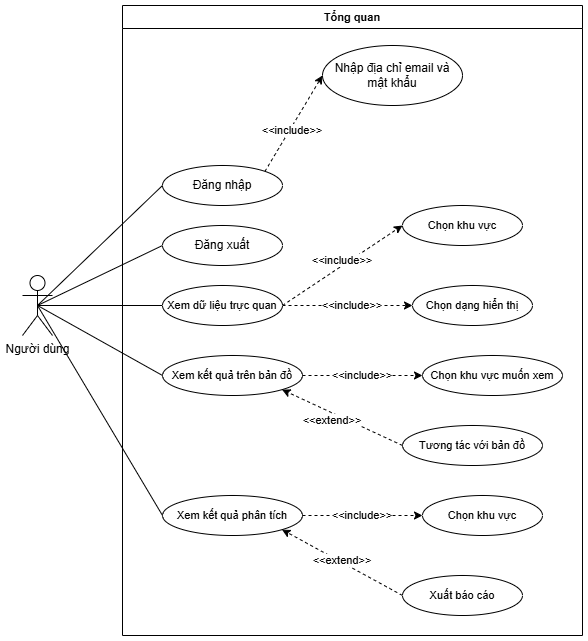
\includegraphics[width=0.9\linewidth]{Images/Usecase tổng quan.drawio.png}
    \caption{Sơ đồ Use Case tổng quan}
\end{figure}

\subsubsubsection{Đăng nhập và đăng xuất}
\begin{figure}[H]
    \centering
    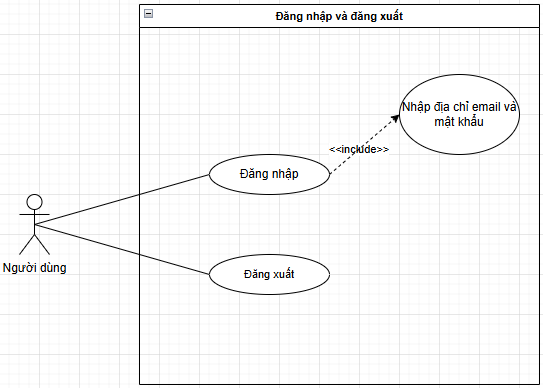
\includegraphics[width=0.9\linewidth]{Images/Usecase1.png}
    \caption{Sơ đồ Use Case đăng nhập và đăng xuất}
\end{figure}
\begin{table}[H]
\centering
\begin{tabular}{|p{0.28\linewidth}|p{0.62\linewidth}|}
\hline
\textbf{Tên use case} & Đăng nhập \\ \hline

\textbf{Mô tả} & 
Cho phép người dùng (đã có tài khoản) truy cập vào hệ thống bằng thông tin xác thực của họ. \\ \hline

\textbf{Tác nhân} & Người dùng (đã có tài khoản). \\ \hline

\textbf{Điều kiện kích hoạt} & 
Người dùng ở trạng thái chưa đăng nhập nhấn vào nút “Đăng nhập”. \\ \hline

\textbf{Điều kiện tiên quyết} &
Người dùng đang ở trạng thái chưa đăng nhập nhưng đã có tài khoản. \\ \hline

\textbf{Điều kiện sau hành động} &
Nếu thành công, người dùng được xác thực và chuyển đến trang tài khoản. Nếu thất bại, hệ thống hiển thị lỗi. \\ \hline

\textbf{Luồng chính} &
1. Người dùng nhấp vào giao diện “Đăng nhập”. \newline
2. Nhập email và mật khẩu. \newline
3. Nhấn “Đăng nhập”. \newline
4. Hệ thống kiểm tra và xác thực thông tin. \newline
5. Hệ thống tạo phiên đăng nhập và chuyển người dùng đến trang chủ. \\ \hline

\textbf{Luồng rẽ nhánh} & 
5a. Email hoặc mật khẩu không chính xác dẫn đến hệ thống báo lỗi và yêu cầu nhập lại. \\ \hline

\textbf{Kết quả} & Phiên đăng nhập được tạo hoặc hiển thị lỗi. \\ \hline
\end{tabular}
\end{table}

\begin{table}[H]
\centering
\begin{tabular}{|p{0.28\linewidth}|p{0.62\linewidth}|}
\hline
\textbf{Tên use case} & Đăng xuất \\ \hline

\textbf{Mô tả} & 
Cho phép người dùng (đã đăng nhập) thoát ra khỏi tài khoản đang đăng nhập. \\ \hline

\textbf{Tác nhân} & Người dùng \\ \hline

\textbf{Điều kiện kích hoạt} &
Người dùng nhấn vào nút “Đăng xuất”. \\ \hline

\textbf{Điều kiện tiên quyết} &
Người dùng đang trong trạng thái đăng nhập. \\ \hline

\textbf{Điều kiện sau hành động} &
Phiên đăng nhập bị hủy và chuyển hướng về trang đăng nhập (trạng thái chưa đăng nhập). \\ \hline

\textbf{Luồng chính} &
1. Người dùng nhấn nút “Đăng xuất”. \newline
2. Hệ thống hủy phiên đăng nhập. \newline
3. Hệ thống xóa thông tin đăng nhập (cookies, local storage nếu có). \newline
4. Chuyển hướng người dùng về trang đăng nhập. \\ \hline

\textbf{Luồng rẽ nhánh} &
Không có. \\ \hline

\textbf{Kết quả} &
Người dùng trở về trạng thái chưa đăng nhập. \\ \hline
\end{tabular}
\end{table}

\subsubsubsection{Trực quan hóa dữ liệu}
\begin{figure}[H]
    \centering
    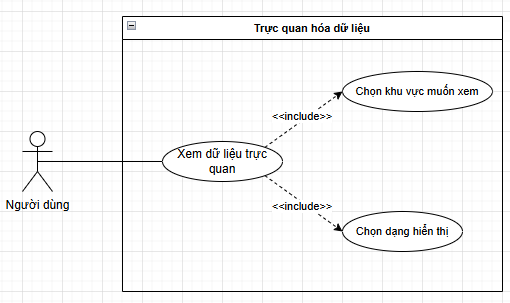
\includegraphics[width=0.9\linewidth]{Images/Usecase2.png}
    \caption{Sơ đồ Use Case trực quan hóa dữ liệu}
\end{figure}
\begin{table}[H]
\centering
\begin{tabular}{|p{0.28\linewidth}|p{0.62\linewidth}|}
\hline
\textbf{Tên use case} & Trực quan hóa dữ liệu \\ \hline

\textbf{Mô tả} & 
Cho phép nhà phân tích quan sát dữ liệu giao thông dưới dạng biểu đồ như: biểu đồ thời gian, biểu đồ phân phối, heatmap, hoặc biểu đồ so sánh nhằm hỗ trợ việc phân tích. \\ \hline

\textbf{Tác nhân} & Người dùng. \\ \hline

\textbf{Điều kiện kích hoạt} & 
Người dùng yêu cầu xem dữ liệu hoặc xem kết quả xử lý dữ liệu ở dạng biểu đồ. \\ \hline

\textbf{Điều kiện tiên quyết} &
Dữ liệu giao thông đã được tiền xử lý và sẵn sàng để hiển thị. \\ \hline

\textbf{Điều kiện sau hành động} &
Biểu đồ hoặc hình ảnh trực quan được tạo và hiển thị để phục vụ phân tích. \\ \hline

\textbf{Luồng chính} &
1. Người dùng chọn khu vực muốn xem (có thể là đoạn đường, phường hoặc quận). \newline
2. Chọn loại biểu đồ muốn hiển thị. \newline
3. Hệ thống xử lý và tạo biểu đồ tương ứng. \newline
4. Biểu đồ được hiển thị cho nhà phân tích xem hoặc lưu lại. \\ \hline

\textbf{Luồng rẽ nhánh} & 
3a. Nếu dữ liệu thiếu hoặc không hợp lệ, hệ thống sẽ hiển thị thông báo lỗi. \\ \hline

\textbf{Kết quả} & Biểu đồ hiển thị thành công hoặc thông báo lỗi nếu dữ liệu không hợp lệ. \\ \hline
\end{tabular}
\end{table}

\subsubsubsection{Hiển thị kết quả phân tích trên bản đồ}
\begin{figure}[H]
    \centering
    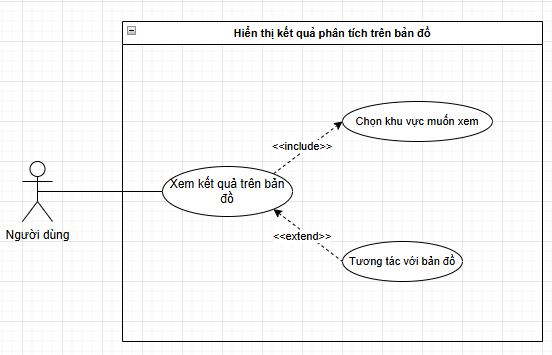
\includegraphics[width=0.9\linewidth]{Images/Usecase3.png}
    \caption{Sơ đồ Use Case hiển thị kết quả phân tích trên bản đồ}
\end{figure}
\begin{table}[H]
\centering
\begin{tabular}{|p{0.28\linewidth}|p{0.62\linewidth}|}
\hline
\textbf{Tên use case} & Hiển thị kết quả phân tích trên bản đồ \\ \hline

\textbf{Mô tả} & 
Cho phép người dùng quan sát kết quả phân tích giao thông trực tiếp trên bản đồ, bao gồm tô màu đoạn đường theo tốc độ, mức độ ùn tắc hoặc các thông số phân tích khác. \\ \hline

\textbf{Tác nhân} & Người dùng. \\ \hline

\textbf{Điều kiện kích hoạt} & 
Người dùng yêu cầu xem kết quả phân tích trên nền bản đồ. \\ \hline

\textbf{Điều kiện tiên quyết} &
Dữ liệu có chứa thông tin không gian (đoạn đường, tọa độ, hoặc dạng network). \\ \hline

\textbf{Điều kiện sau hành động} &
Hiển thị bản đồ với các tuyến đường được tô màu theo giá trị tương ứng; nhà phân tích có thể quan sát và ghi nhận kết quả. \\ \hline

\textbf{Luồng chính} &
1. Người dùng chọn khu vực cần hiển thị. \newline
2. Hệ thống ánh xạ dữ liệu lên bản đồ. \newline
3. Bản đồ được tạo và tô màu theo tốc độ hoặc mức độ ùn tắc. \newline
4. Người dùng tương tác, xem chi tiết hoặc lưu hình ảnh bản đồ. \\ \hline

\textbf{Luồng rẽ nhánh} & 
2a. Thiếu dữ liệu vị trí, hệ thống không thể tạo bản đồ và hiển thị thông báo lỗi. \\ \hline

\textbf{Kết quả} & Bản đồ được hiển thị và sẵn sàng phục vụ phân tích. \\ \hline
\end{tabular}
\end{table}

\subsubsubsection{Xem và xuất báo cáo kết quả phân tích}
\begin{figure}[H]
    \centering
    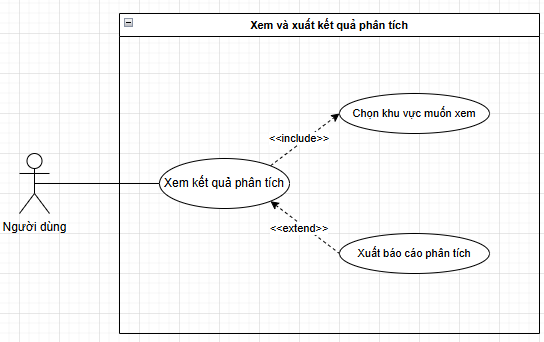
\includegraphics[width=0.9\linewidth]{Images/Usecase4.png}
    \caption{Sơ đồ Use Case xem và xuất kết quả phân tích}
\end{figure}
\begin{table}[H]
\centering
\begin{tabular}{|p{0.28\linewidth}|p{0.62\linewidth}|}
\hline
\textbf{Tên use case} & Xem kết quả phân tích \\ \hline

\textbf{Mô tả} & 
Cho phép người dùng xem các kết quả phân tích tình trạng giao thông, bao gồm các biểu đồ, bản đồ trực quan, thống kê hoặc chỉ số được hệ thống tạo ra từ dữ liệu giao thông đã xử lý. \\ \hline

\textbf{Tác nhân} & Người dùng. \\ \hline

\textbf{Điều kiện kích hoạt} & 
Người dùng truy cập vào mục xem kết quả phân tích hoặc chọn một khu vực để hiển thị kết quả. \\ \hline

\textbf{Điều kiện tiên quyết} &
Hệ thống đã xử lý dữ liệu và tạo ra kết quả phân tích tương ứng. \\ \hline

\textbf{Điều kiện sau hành động} &
Kết quả phân tích được hiển thị dưới dạng biểu đồ, bản đồ hoặc số liệu thống kê. \\ \hline

\textbf{Luồng chính} &
1. Người dùng truy cập chức năng xem kết quả phân tích. \newline
2. Người dùng chọn khu vực muốn xem. \newline
3. Hệ thống truy xuất kết quả phân tích tương ứng từ cơ sở dữ liệu hoặc mô-đun xử lý. \newline
4. Hệ thống hiển thị kết quả dưới dạng biểu đồ, bản đồ hoặc bảng số liệu. \\ \hline

\textbf{Luồng rẽ nhánh} & 
3a. Nếu chưa có kết quả phân tích cho khu vực đã chọn, hệ thống thông báo "Chưa có dữ liệu phân tích". \\ \hline

\textbf{Kết quả} & 
Người dùng xem được kết quả phân tích hoặc nhận thông báo nếu dữ liệu không có sẵn. \\ \hline
\end{tabular}
\end{table}

\begin{table}[H]
\centering
\begin{tabular}{|p{0.28\linewidth}|p{0.62\linewidth}|}
\hline
\textbf{Tên use case} & Xuất báo cáo phân tích \\ \hline

\textbf{Mô tả} & 
Cho phép nhà phân tích xuất các kết quả phân tích (biểu đồ, bảng số liệu, bản đồ, thống kê) thành tệp tin như PDF, CSV hoặc hình ảnh phục vụ trình bày hoặc báo cáo nghiên cứu. \\ \hline

\textbf{Tác nhân} & Người dùng. \\ \hline

\textbf{Điều kiện kích hoạt} & 
Người dùng yêu cầu lưu lại kết quả phân tích dưới dạng tệp. \\ \hline

\textbf{Điều kiện tiên quyết} &
Kết quả phân tích đã được tạo và sẵn sàng để xuất file. \\ \hline

\textbf{Điều kiện sau hành động} &
Hệ thống tạo file báo cáo hoặc hình ảnh và cung cấp cho người dùng để tải xuống. \\ \hline

\textbf{Luồng chính} &
1. Người dùng chọn loại file báo cáo muốn xuất (PDF, CSV, hình ảnh...). \newline
2. Hệ thống tổng hợp dữ liệu và biểu đồ liên quan. \newline
3. Hệ thống tạo tệp báo cáo. \newline
4. Người dùng tải xuống tệp. \\ \hline

\textbf{Luồng rẽ nhánh} & 
2a. Thiếu dữ liệu đầu vào, hệ thống không thể tạo báo cáo và thông báo lỗi. \\ \hline

\textbf{Kết quả} & Tệp báo cáo được tạo thành công hoặc hiển thị lỗi nếu thất bại. \\ \hline
\end{tabular}
\end{table}

\subsubsubsection{Dự báo lan truyền ùn tắc giao thông}

\begin{figure}[H]
    \centering
    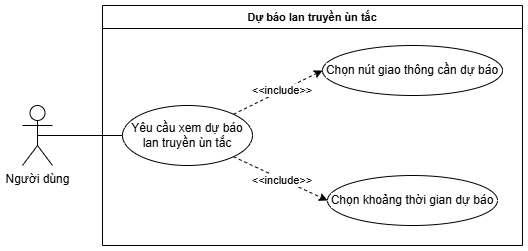
\includegraphics[width=0.9\linewidth]{Images/Usecase5.png}
    \caption{Sơ đồ Use Case dự báo ùn tắc giao thông}
\end{figure}

\begin{table}[H]
\centering
\begin{tabular}{|p{0.28\linewidth}|p{0.62\linewidth}|}
\hline
\textbf{Use case id} & 7 \\ \hline

\textbf{Tên use case} & Dự báo lan truyền ùn tắc giao thông \\ \hline

\textbf{Mô tả} & 
Cho phép người dùng xem dự báo việc một nút giao thông bị tắc nghẽn sẽ ảnh hưởng và lan truyền đến các nút giao thông lân cận nào trong mạng lưới giao thông, đồng thời ước lượng khoảng thời gian lan truyền. \\ \hline

\textbf{Tác nhân} & Người dùng. \\ \hline

\textbf{Điều kiện kích hoạt} & 
Người dùng chọn một nút giao thông đang hoặc có nguy cơ bị tắc nghẽn và yêu cầu hệ thống thực hiện dự báo lan truyền. \\ \hline

\textbf{Điều kiện tiên quyết} &
Dữ liệu giao thông đã được thu thập và tiền xử lý. Mạng lưới giao thông đã được xây dựng. Hệ thống có mô hình hoặc thuật toán dự báo lan truyền ùn tắc.\\ \hline

\textbf{Điều kiện sau hành động} &
Kết quả dự báo được tạo ra, bao gồm danh sách các nút bị ảnh hưởng và thời gian lan truyền tương ứng. \\ \hline

\textbf{Luồng chính} &
1. Người dùng chọn nút giao thông cần dự báo. \newline
2. Người dùng chọn khoảng thời gian dự báo. \newline
3. Hệ thống truy xuất dữ liệu giao thông và cấu trúc mạng lưới liên quan. \newline
4. Hệ thống thực hiện mô phỏng hoặc mô hình dự báo lan truyền ùn tắc. \newline
5. Hệ thống xác định các nút giao thông bị ảnh hưởng và thời gian lan truyền. \newline
6. Kết quả dự báo được hiển thị dưới dạng bản đồ, biểu đồ hoặc bảng số liệu. \\ \hline

\textbf{Luồng rẽ nhánh} &
4a. Nếu dữ liệu không đủ hoặc mô hình không hội tụ, hệ thống hiển thị thông báo lỗi hoặc cảnh báo độ tin cậy thấp. \\ \hline

\textbf{Kết quả} &
Người dùng quan sát được phạm vi lan truyền ùn tắc và thời gian ảnh hưởng, hoặc nhận thông báo nếu dự báo không khả thi. \\ \hline
\end{tabular}
\end{table}

\subsubsection{Mô hình hóa quy trình nghiệp vụ}

\subsubsubsection{Activity diagram}
\begin{figure}[H]
    \centering
    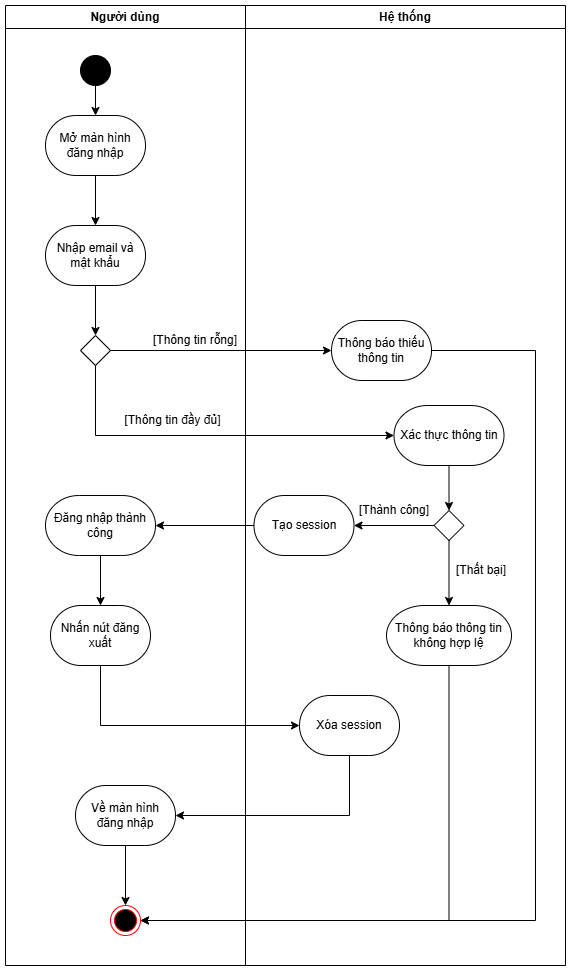
\includegraphics[width=0.7\linewidth]{Images/Act đăng nhập, đăng xuất.png}
    \caption{Sơ đồ Activity đăng nhập, đăng xuất}
\end{figure}

\begin{figure}[H]
    \centering
    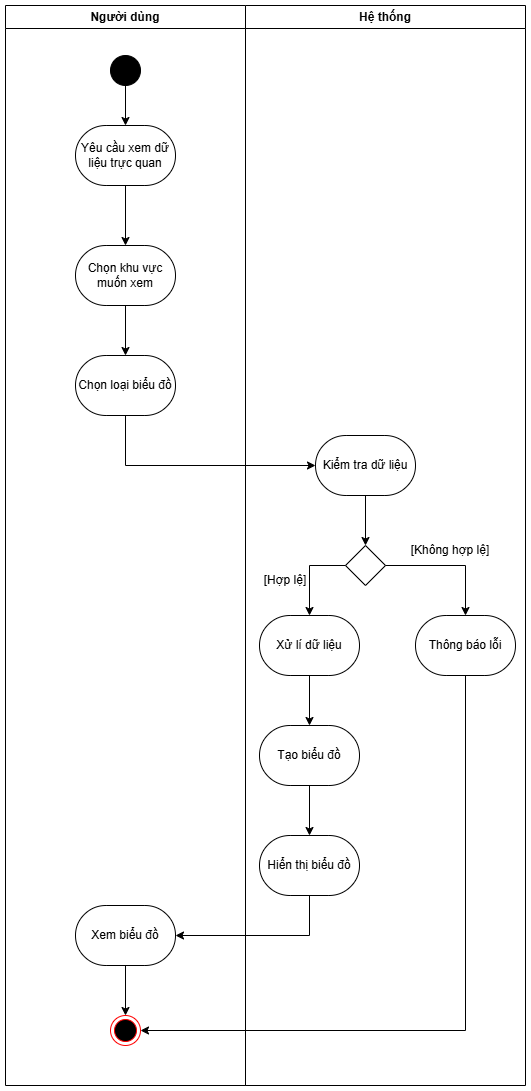
\includegraphics[width=0.7\linewidth]{Images/Act trực quan hóa dữ liệu.png}
    \caption{Sơ đồ Activity trực quan hóa dữ liệu}
\end{figure}

\begin{figure}[H]
    \centering
    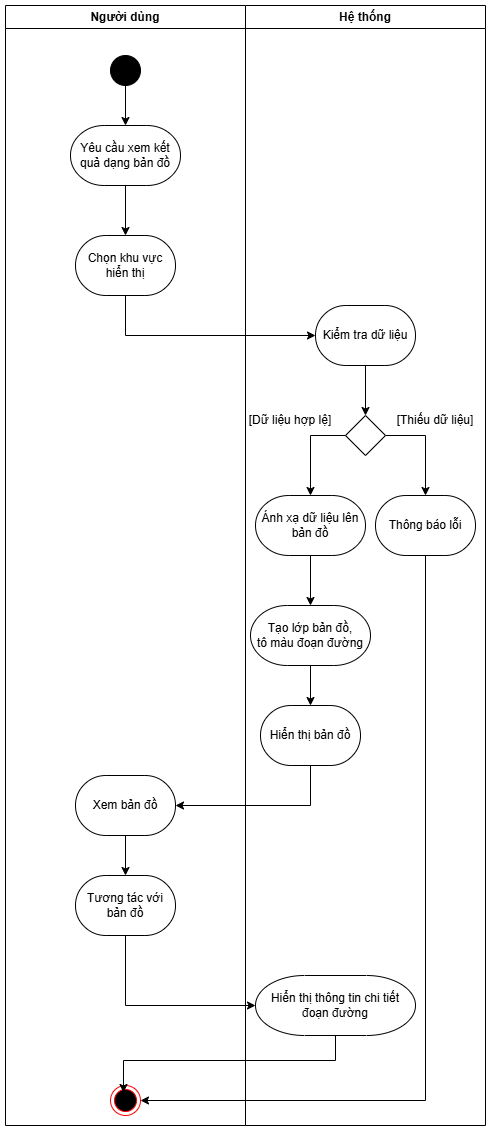
\includegraphics[width=0.6\linewidth]{Images/Act xem kết quả dạng bản đồ.png}
    \caption{Sơ đồ Activity xem kết quả dạng bản đồ}
\end{figure}

\begin{figure}[H]
    \centering
    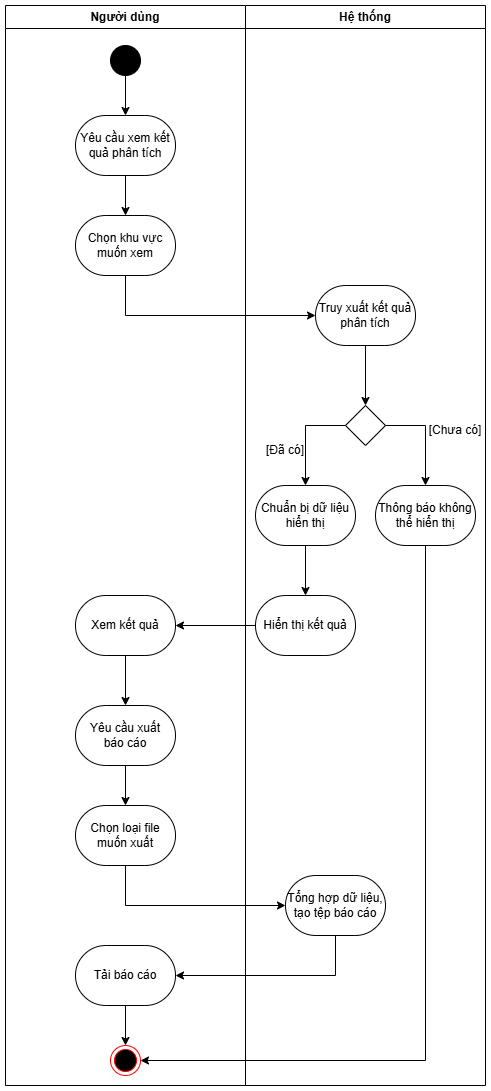
\includegraphics[width=0.6\linewidth]{Images/Act xem và xuất báo cáo.png}
    \caption{Sơ đồ Activity xem và xuất kết quả phân tích}
\end{figure}

\begin{figure}[H]
    \centering
    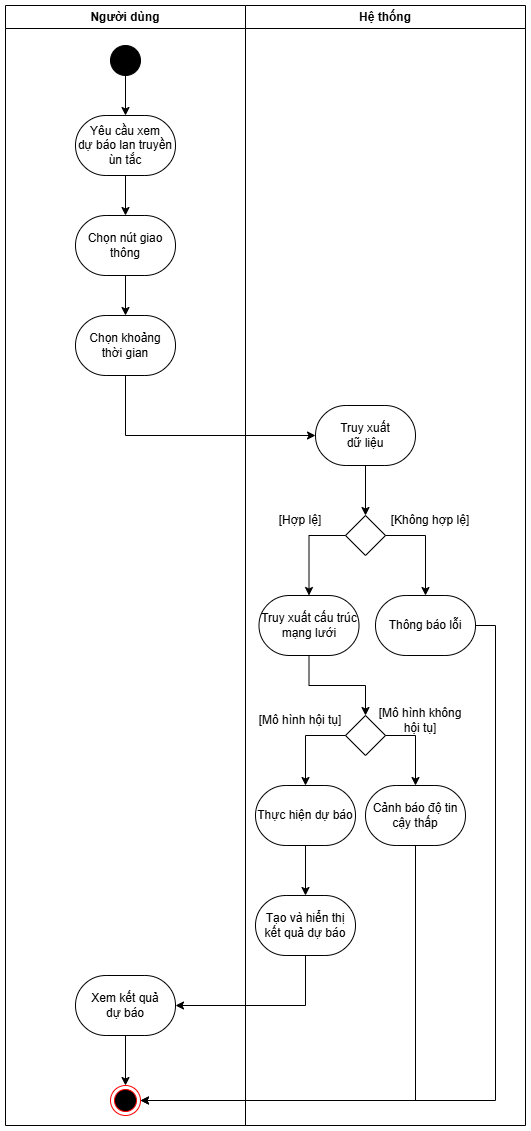
\includegraphics[width=0.7\linewidth]{Images/Act dự báo lan truyền ùn tắc.png}
    \caption{Sơ đồ Activity dự báo lan truyền ùn tắc giao thông}
\end{figure}
\subsubsubsection{Sequence diagram}

\begin{figure}[H]
    \centering
    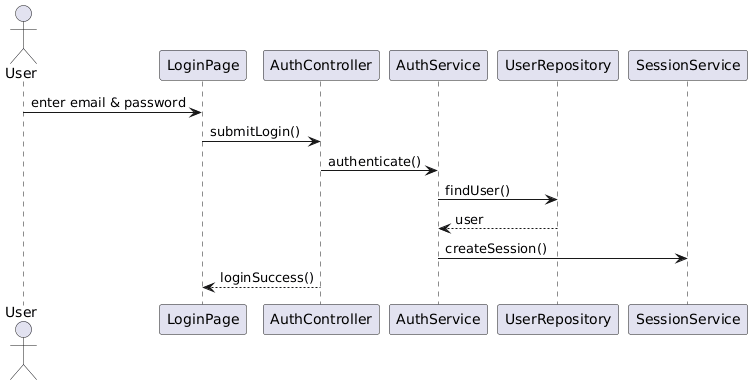
\includegraphics[width=1\linewidth]{Images/Sequence diagram/Login.png}
    \caption{Sơ đồ Sequence đăng nhập}
\end{figure}

\begin{figure}[H]
    \centering
    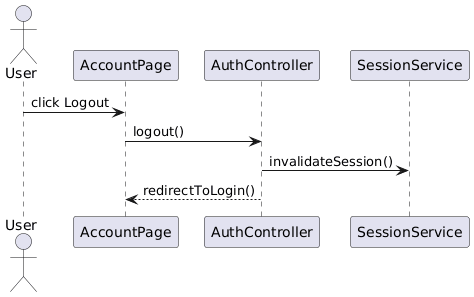
\includegraphics[width=0.9\linewidth]{Images/Sequence diagram/Logout.png}
    \caption{Sơ đồ Sequence đăng xuất}
\end{figure}

\begin{figure}[H]
    \centering
    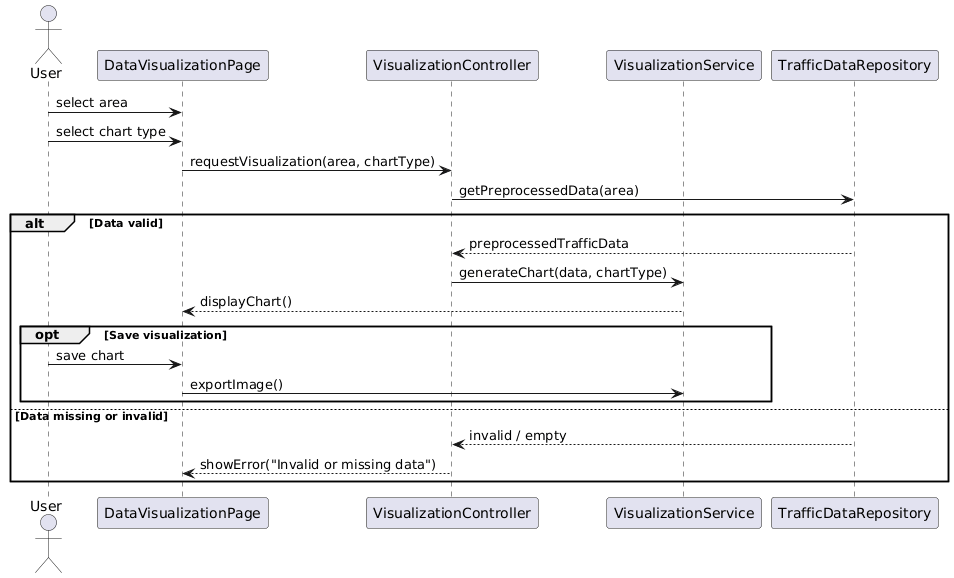
\includegraphics[width=1\linewidth]{Images/Sequence diagram/Visualize Data.png}
    \caption{Sơ đồ Sequence trực quan hóa dữ liệu}
\end{figure}

\begin{figure}[H]
    \centering
    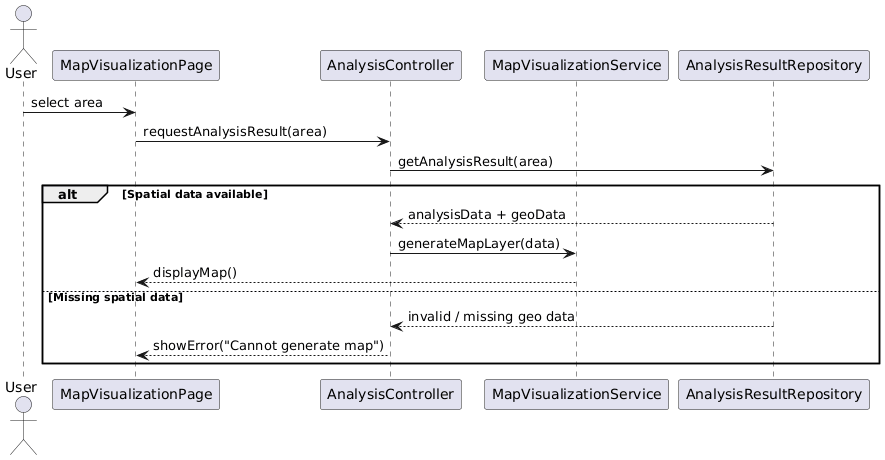
\includegraphics[width=1\linewidth]{Images/Sequence diagram/Analysis Results Map.png}
    \caption{Sơ đồ Sequence xem kết quả dạng bản đồ}
\end{figure}

\begin{figure}[H]
    \centering
    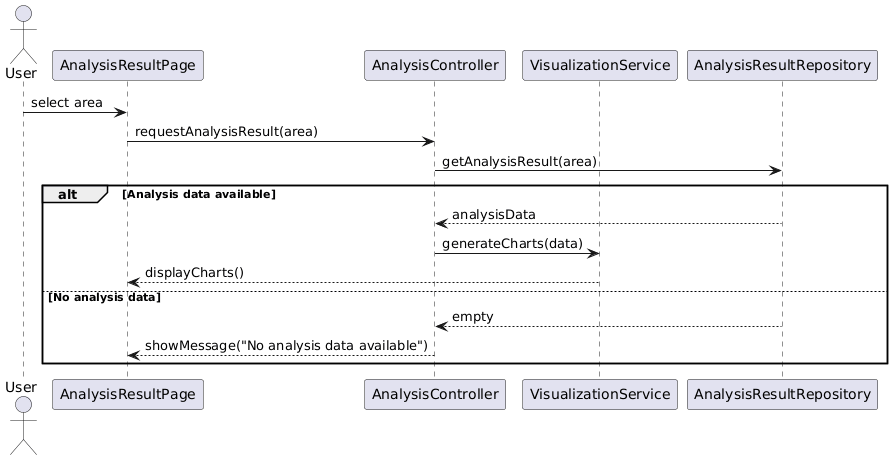
\includegraphics[width=1\linewidth]{Images/Sequence diagram/View Analysis Results.png}
    \caption{Sơ đồ Sequence xem kết quả phân tích}
\end{figure}

\begin{figure}[H]
    \centering
    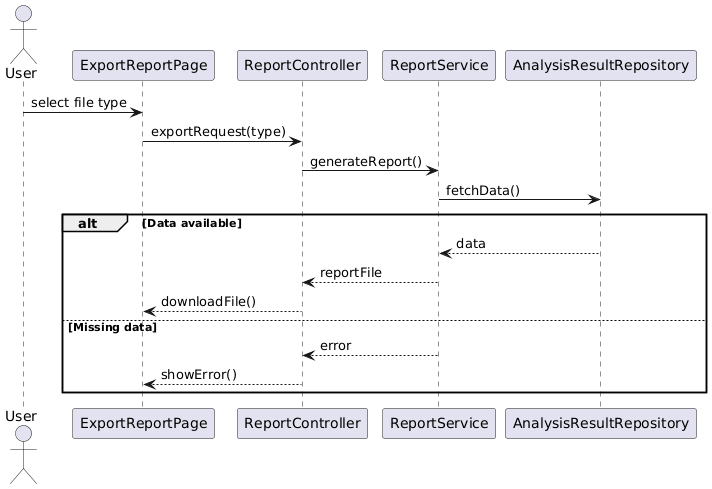
\includegraphics[width=1\linewidth]{Images/Sequence diagram/Export Report.png}
    \caption{Sơ đồ Sequence xuất kết quả phân tích}
\end{figure}

\begin{figure}[H]
    \centering
    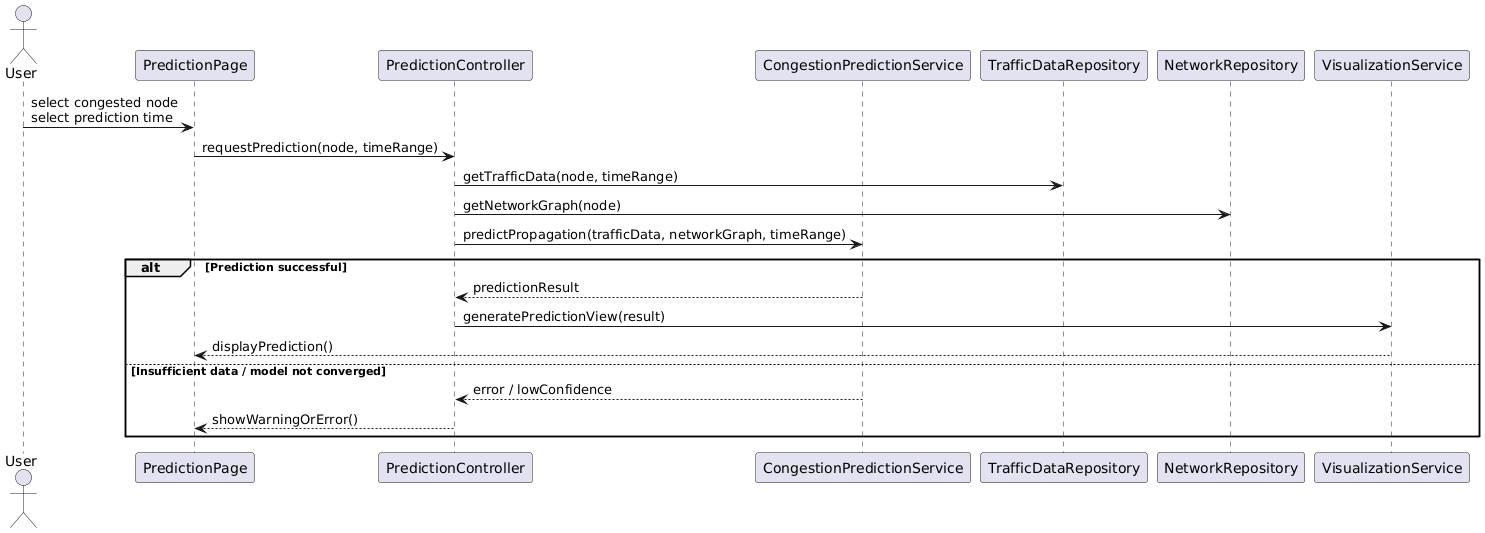
\includegraphics[width=1\linewidth]{Images/Sequence diagram/Predict.png}
    \caption{Sơ đồ Sequence dự báo lan truyền ùn tắc giao thông}
\end{figure}
\newpage
\input{Contents/7_HienThucVaKiemThu}
\newpage
\input{Contents/8_DanhGiaHeThong}
\newpage
\section{Tổng kết}
\subsection{Kết quả đạt được}
\subsection{Hướng phát triển}
% (all limitations of your current work are described here and then linked to your future works. For
% the first phase, they are included in the plan for the next phase.)
\newpage
\section*{Kế hoạch thực hiện Đồ án tốt nghiệp}
Dựa trên cơ sở kết quả đạt được từ Đồ án Chuyên ngành, nhóm lên kế hoạch thực hiện Đồ án tốt nghiệp trong thời hạn 15 tuần như sau:

\subsubsection*{Tuần 1--2: Tổng quan và kế thừa kết quả}
\begin{itemize}
    \item Rà soát và hệ thống hóa các kết quả đạt được từ đồ án chuyên ngành.
    \item Đánh giá ưu điểm và hạn chế của mô hình phân tích và dự báo hiện tại.
    \item Xác định mục tiêu, phạm vi và nội dung cần mở rộng trong đồ án tốt nghiệp.
\end{itemize}

\subsubsection*{Tuần 3--4: Mở rộng và hoàn thiện dữ liệu giao thông}
\begin{itemize}
    \item Khảo sát và tích hợp thêm các nguồn dữ liệu giao thông mới.
    \item Mở rộng dữ liệu theo phạm vi không gian và thời gian.
    \item Tiếp tục thực hiện tiền xử lý, chuẩn hóa và tổ chức dữ liệu phục vụ phân tích và dự báo.
\end{itemize}

\subsubsection*{Tuần 5--7: Cải tiến mô hình phân tích và dự báo lan truyền ùn tắc}
\begin{itemize}
    \item Nghiên cứu và cải tiến mô hình dự báo lan truyền ùn tắc hiện tại.
    \item Mở rộng khả năng dự báo về mặt thời gian so với mô hình ban đầu.
    \item Thực hiện so sánh các mô hình hoặc phương pháp dự báo khác nhau.
\end{itemize}

\subsubsection*{Tuần 8--9: Đánh giá và phân tích kết quả mô hình}
\begin{itemize}
    \item Đánh giá mô hình dự báo bằng các thước đo như MAE, RMSE.
    \item Phân tích khả năng mô hình hóa sự lan truyền ùn tắc trong mạng lưới giao thông.
    \item Thảo luận và rút ra nhận xét về hiệu quả của các mô hình.
\end{itemize}

\subsubsection*{Tuần 10--11: Hiện thực hóa hệ thống hỗ trợ phân tích}
\begin{itemize}
    \item Hiện thực các chức năng chính của hệ thống dựa trên thiết kế đã đề xuất.
    \item Tích hợp mô hình phân tích và dự báo vào hệ thống.
    \item Xây dựng giao diện người dùng phục vụ việc trực quan hóa dữ liệu và kết quả.
\end{itemize}

\subsubsection*{Tuần 12--13: Hoàn thiện chức năng và trực quan hóa}
\begin{itemize}
    \item Hoàn thiện các chức năng trực quan hóa bằng biểu đồ và bản đồ.
    \item Bổ sung chức năng xuất báo cáo và lưu kết quả phân tích.
    \item Kiểm thử hệ thống với các kịch bản dữ liệu khác nhau.
\end{itemize}

\subsubsection*{Tuần 14: Đánh giá hệ thống và thực nghiệm}
\begin{itemize}
    \item Đánh giá hiệu năng và tính ổn định của hệ thống.
    \item Thực hiện các thí nghiệm minh họa và phân tích kết quả.
    \item Tổng hợp ưu điểm và hạn chế của hệ thống.
\end{itemize}

\subsubsection*{Tuần 15: Hoàn thiện báo cáo và chuẩn bị bảo vệ}
\begin{itemize}
    \item Hoàn thiện báo cáo đồ án tốt nghiệp.
    \item Chuẩn bị slide và nội dung thuyết trình.
    \item Rà soát và chỉnh sửa toàn bộ tài liệu liên quan.
\end{itemize}
\newpage
%%%%%%%%%%%%%%%%%OUTRO%%%%%%%%%%%%%%%%%%%
\begin{thebibliography}{99}

\bibitem{Saberi2020}
M.~Saberi, H.~Hamedmoghadam, M.~Ashfaq \textit{et al.},
``A simple contagion process describes spreading of traffic jams in urban networks,''
\textit{Nature Communications}, vol.~11, no.~1, pp.~15353, 2020.

\bibitem{Zhao2020}
L.~Zhao, Y.~Song, C.~Zhang, Y.~Liu, P.~Wang, T.~Lin, M.~Deng, H.~Li,
``T-GCN: A temporal graph convolutional network for traffic prediction,''
\textit{IEEE Transactions on Intelligent Transportation Systems},
vol.~21, no.~9, pp.~3848--3858, 2020.

\bibitem{Nagy2021}
A.~M.~Nagy, V.~Simon,
``Improving traffic prediction using congestion propagation patterns in smart cities,''
\textit{Advanced Engineering Informatics},
vol.~50, pp.~101343, 2021.

\bibitem{Li2020}
C.~Li, W.~Yue, G.~Mao, Z.~Xu,
``Congestion propagation based bottleneck identification in urban road networks,''
\textit{IEEE Transactions on Vehicular Technology},
vol.~69, no.~5, pp.~4827--4837, 2020.

\bibitem{Zhang2020}
Y.~Zhang, Y.~Li, X.~Zhou, X.~Kong, J.~Luo,
``Curb-GAN: Conditional urban traffic estimation through spatio-temporal generative adversarial networks,''
in \textit{Proceedings of the 26th ACM SIGKDD International Conference on Knowledge Discovery \& Data Mining},
pp.~842--852, 2020.

\bibitem{Ermagun2017}
A.~Ermagun, S.~Chatterjee, D.~Levinson,
``Using temporal detrending to observe the spatial correlation of traffic,''
\textit{PLOS ONE},
vol.~12, no.~5, e0176853, 2017.

\bibitem{Xu2023}
Y.~Xu, X.~Cai, E.~Wang, W.~Liu, Y.~Yang, F.~Yang,
``Dynamic traffic correlations based spatio-temporal graph convolutional network for urban traffic prediction,''
\textit{Information Sciences},
vol.~621, pp.~580--595, 2023.

\bibitem{Lampo2021}
A.~Lampo, J.~Borge-Holthoefer, S.~G{\'o}mez, A.~Sol{\'e}-Ribalta,
``Emergence of spatial transitions in urban congestion dynamics,''
\textit{Applied Network Science},
vol.~6, no.~1, pp.~1--19, 2021.

\bibitem{Chen2024}
J.~Chen, Y.~Wu,
``The propagation of congestion on transportation networks analyzed by the percolation process,''
\textit{Mathematics},
vol.~12, no.~20, pp.~3247, 2024.

\bibitem{Vlahogianni2014}
E.~I.~Vlahogianni, M.~G.~Karlaftis, J.~C.~Golias,
``Short-term traffic forecasting: Where we are and where we’re going,''
\textit{Transportation Research Part C},
vol.~43, pp.~3--19, 2014.

\bibitem{Treiber2013}
M.~Treiber, A.~Kesting,
\textit{Traffic Flow Dynamics: Data, Models and Simulation},
Springer, 2013.

\bibitem{Wu2021Survey}
Z.~Wu, S.~Pan, F.~Chen, G.~Long, C.~Zhang, P.~Yu,
``A comprehensive survey on graph neural networks,''
\textit{IEEE Transactions on Neural Networks and Learning Systems},
vol.~32, no.~1, pp.~4--24, 2021.

\bibitem{Yu2018STGCN}
B.~Yu, H.~Yin, Z.~Zhu,
``Spatio-temporal graph convolutional networks: A deep learning framework for traffic forecasting,''
in \textit{Proceedings of IJCAI},
pp.~3634--3640, 2018.

\bibitem{Kreps2011Kafka}
J.~Kreps, N.~Narkhede, J.~Rao,
``Kafka: A distributed messaging system for log processing,''
in \textit{Proceedings of NetDB},
2011.

\bibitem{Akidau2015Streaming}
T.~Akidau, R.~Bradshaw, C.~Chambers \textit{et al.},
``The dataflow model: A practical approach to balancing correctness, latency, and cost in massive-scale, unbounded, out-of-order data processing,''
\textit{Proceedings of VLDB},
vol.~8, no.~12, pp.~1792--1803, 2015.

\bibitem{Zheng2015Urban}
Y.~Zheng,
``Trajectory data mining: An overview,''
\textit{ACM Transactions on Intelligent Systems and Technology},
vol.~6, no.~3, pp.~29, 2015.

\bibitem{ITSHandbook}
U.S. Department of Transportation,
\textit{Intelligent Transportation Systems Architecture and Standards},
2017.

\end{thebibliography}

\newpage
\appendix
\section*{PHỤ LỤC}
\addcontentsline{toc}{section}{PHỤ LỤC}

\section{Mô tả chi tiết dữ liệu TomTom}
Phụ lục này trình bày cấu trúc dữ liệu lịch sử thu thập từ TomTom Statistics API,
bao gồm vận tốc trung bình, mức độ tắc nghẽn và chỉ số độ tin cậy theo từng đoạn đường.

\section{Chi tiết thuật toán mô phỏng lan truyền tắc nghẽn}
Thuật toán~\ref{alg:congestion_propagation} mô phỏng quá trình lan truyền tắc nghẽn
trên đồ thị nhân quả, dựa trên độ trễ lan truyền và xác suất ảnh hưởng giữa các nút.

\section{Kiến trúc hệ thống triển khai}
Hình~\ref{fig:system_deployment} mô tả kiến trúc tổng thể của hệ thống,
bao gồm tầng thu thập dữ liệu, xử lý luồng, mô hình học máy và giao diện người dùng.
\end{document}


